\documentclass[12pt]{book}
\usepackage[dvipsnames]{xcolor}
\usepackage{amssymb,latexsym}
\usepackage{graphicx}
\usepackage{listings}
\usepackage{xcolor}
\usepackage[spanish,mexico,es-nolayout]{babel}
\usepackage[latin1]{inputenc}
\usepackage[spanish]{babel}
\usepackage{amsmath}
\usepackage{mdframed}
\usepackage{booktabs}
\usepackage{algorithm}
\usepackage{algorithmic}
\DeclareMathOperator{\tr}{tr}
% \usepackage{amssymb}
\usepackage{amsthm}
%\usepackage{graphicx}
\usepackage{color}
\usepackage{tikz}
\usepackage{tkz-berge}
\usetikzlibrary{positioning,backgrounds}
\usepackage{makeidx}
\usepackage{url}
\usepackage{xspace}
\usepackage{tocbibind}
\usepackage{rotating}
\usepackage{float}
\usepackage{young}
\usepackage{ytableau}
\usepackage{mathtools}
\usepackage[all]{xy}
\DeclarePairedDelimiter\ceil{\lceil}{\rceil}
\DeclarePairedDelimiter\floor{\lfloor}{\rfloor}
% ver http://gilmation.com/articles/latex-margins-for-book-binding/
% y http://tex.stackexchange.com/questions/50258/margins-of-book-class
\usepackage[margin=3.5cm]{geometry}
\geometry{bindingoffset=1cm}

%\usepackage{babelbib}

\usetikzlibrary{positioning,shapes,fit,arrows,decorations.pathmorphing}
\definecolor{myblue}{RGB}{56,94,141}


\newtheorem{theorem}{Teorema}[section]
\newtheorem{corollary}[theorem]{Corolario}
\newtheorem{proposition}[theorem]{Proposición}

\theoremstyle{definition}

\newtheorem{definition}[theorem]{Definición}
\newtheorem{notation}[theorem]{Notación}
\newtheorem{example}[theorem]{Ejemplo}
\newtheorem{lemma}[theorem]{Lema}

\newcounter{in}
\newcounter{ini}

\DeclareMathOperator{\Cay}{Cay}
\DeclareMathOperator{\diam}{diam}
\DeclareMathOperator{\Stab}{Stab}
\DeclareMathOperator{\Aut}{Aut}
\DeclareMathOperator{\orb}{Orb}
\DeclareMathOperator{\im}{im}
\DeclareMathOperator{\sgn}{sgn}

\newcommand{\GAP}{\textsf{GAP}\xspace}
\newcommand{\GRAPE}{\textsf{GRAPE}\xspace}

\makeindex

\newcommand{\elespacio}{1.4cm}

\newcommand{\rep}{A}
%New colors defined below
\definecolor{codegreen}{rgb}{0,0.6,0}
\definecolor{codegray}{rgb}{0.5,0.5,0.5}
\definecolor{codepurple}{rgb}{0.58,0,0.82}
\definecolor{backcolour}{rgb}{0.95,0.95,0.92}

%Code listing style named "mystyle"
\lstdefinestyle{mystyle}{
  backgroundcolor=\color{backcolour},   commentstyle=\color{codegreen},
  keywordstyle=\color{magenta},
  numberstyle=\tiny\color{codegray},
  stringstyle=\color{codepurple},
  basicstyle=\ttfamily\footnotesize,
  breakatwhitespace=false,         
  breaklines=true,                 
  captionpos=b,                    
  keepspaces=true,                 
  numbers=left,                    
  numbersep=5pt,                  
  showspaces=false,                
  showstringspaces=false,
  showtabs=false,                  
  tabsize=2
}
\begin{document}
\mainmatter 
\begin{titlepage}
  \begin{center}
    \null
    \vspace*{\fill}

    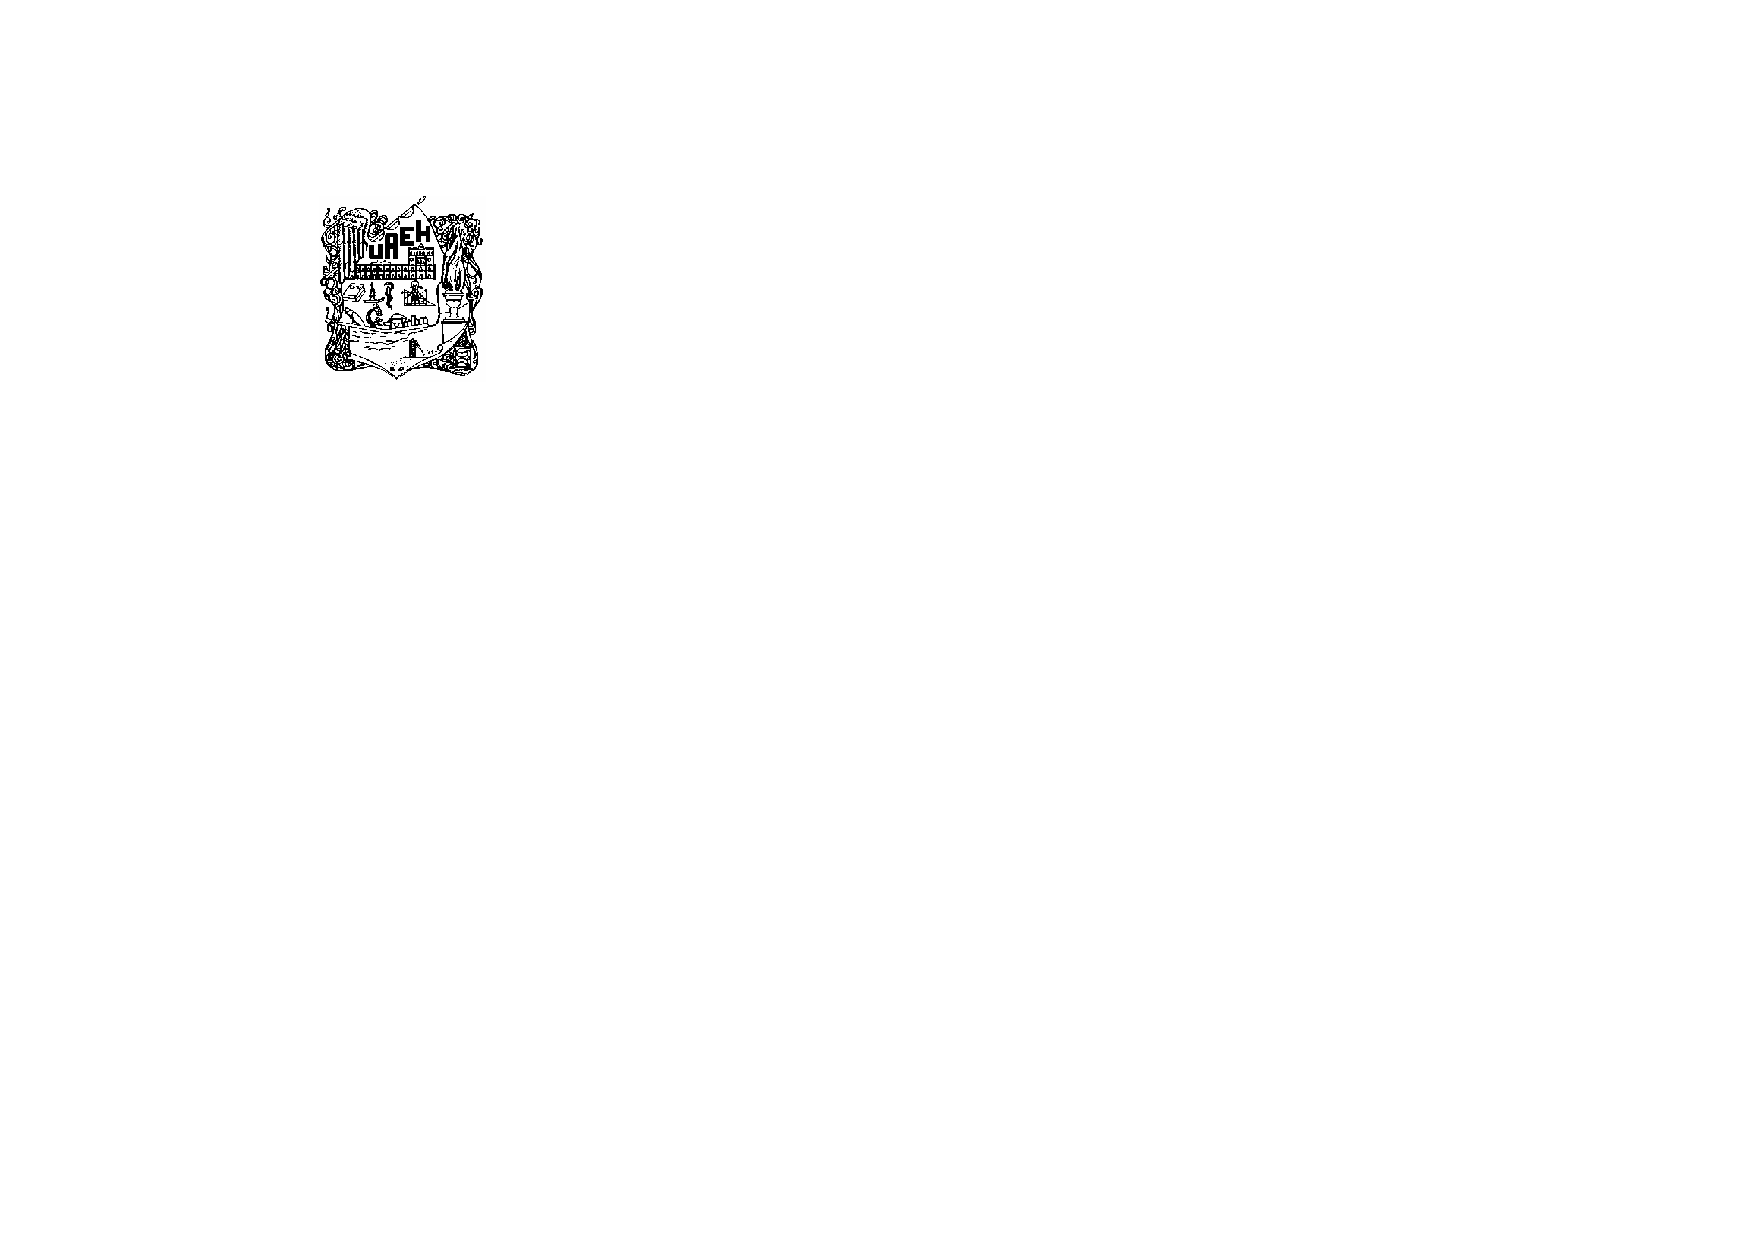
\includegraphics[scale=1.2,bb=55 20 0 0]{escudouaeh.pdf}

    \vspace*{\elespacio}

    \textsc{Universidad Autónoma del Estado de Hidalgo}

    \textsc{Instituto de Ciencias Básicas e Ingeniería}

    \textsc{Área Académica de Matemáticas y Física}

    \vspace*{\elespacio}

    {\Huge\bfseries Un enfoque computacional a la representación del grupo simétrico en homologías\par}

    \vspace*{\elespacio}

    {\large Tesis que para obtener el título de}

    \vspace*{\elespacio}

    {\Large\textsc{Maestro en Matemáticas}}

    \vspace*{\elespacio}

    {\large presenta}

    \vspace*{\elespacio}

    {\Huge Manuel Campero Jurado}

    \vspace*{\elespacio}

    {\large bajo la dirección de}

    \bigskip

    {\Large Dr.~Rafael Villarroel Flores}

    \bigskip

    {Pachuca, Hidalgo. Julio del 2021.}

    \vspace*{\fill}

  \end{center}
\end{titlepage}

\thispagestyle{empty}

\tableofcontents

\newpage

\begin{flushleft}
  {\bfseries\Large Resumen}
\end{flushleft}

En esta tesis se presentan los resultados de ciertos cálculos obtenidos por medio de una biblioteca realizada en
Python. La biblioteca calcula la descomposición en irreducibles de un
$S_n$-módulo $\widetilde H_{k}(\Delta)$, donde $\Delta$ es un complejo
simplicial en el cual los elementos del grupo simétrico actúan como
mapeos simpliciales sobre los vértices. En particular, este trabajo se
interesa por complejos simpliciales que provienen como complejos simpliciales de completas de gráficas.
Más aún, específicamente nos ocuparemos de los complementos de las gráficas de líneas de las gráficas completas
$G_n=\overline{L(K_n)}$. En ese caso, el complejo simplicial de subgráficas completas $\Delta(G_n)$ es el complejo de emparejamientos o matching complex $M_n$, el cual es
bien conocido. También consideraremos al complejo simplicial $K(M_n)$, que denota el
complejo simplicial de la gráfica de clanes de $G_n$. Además se busca
encontrar una fórmula que descomponga al $S_n$-módulo $\widetilde
H_{k}(K(M_n))$ en submódulos irreducibles, así como Bouc
\cite{MR756517} lo realizó para $\widetilde H_{k}(M_n)$.

\vspace{2cm}

\begin{flushleft}
  {\bfseries\Large Abstract}
\end{flushleft}

In this thesis we present results of some calculations obtained by using a library made in Python. This library
allows us to calculate the decomposition into irreducibles of the
$S_n$-module $\widetilde H_{k}(\Delta)$, where $\Delta$ is a
simplicial complex in which the elements of the symmetric group act as
simplicial mappings on the vertices. In particular in this thesis we are
interested in simplicial complexes coming from a graph, specifically
from the complements of the line graphs of the complete graphs $G_n=\overline{L(K_n)}$. In this case, the simplicial complex of complete subgraphs $\Delta(G_n)$ is the matching
complex $M_n$, which is well known. We will also consider the simplicial complex $K(M_n)$,
that denotes the simplicial complex of the clique graph of $G_n$. In
addition, we intend to find a formula that decomposes the
$S_n$-module $\widetilde H_{k}(K(M_n))$ into irreducible submodules,
in a similar manner to that of Bouc \cite{MR756517} in the case of
$\widetilde H_{k}(M_n)$.

 \newpage \thispagestyle{empty}
 
 \chapter*{Introducción}

 Una idea que generalmente aparece en la ciencia es que las grandes
 estructuras pueden ser comprendidas por medio de sus pedazos más
 pequeños. Lo mismo ocurre con la teoría de las
 representaciones. Algunas representaciones se construyen a partir de
 otras más pequeñas, mientras que otras son indivisibles. Esta es la
 distinción entre las representaciones reducibles y representaciones
 irreducibles, algunas de las cuales estudiaremos en este
 trabajo. Sin embargo en este escenario primero es necesario
 determinar con precisión lo que significan estas piezas o
 sub-objetos.

 En la primera sección se presenta la acción de un grupo $G$ en un
 $\mathbb{C}$-espacio vectorial $V$ de dimensión finita, lo cual conduce a definir un
 $G$-módulo. Mientras que una representación del grupo $G$ en el
 espacio vectorial $V$ es un homomorfismo de grupos $G \to GL(V)$,
 donde $GL(V)$ es el grupo de transformaciones lineales invertibles
 $V \to V$. Si el homomorfismo $G \to GL(V)$ es inyectivo, tenemos que
 $G$ es isomorfo a un subgrupo de $GL(V)$, es decir, hemos hallado una
 ``representación'' de los elementos de $G$ como transformaciones
 lineales $V \to V$. Sin embargo las propiedades del homomorfismo
 $G \to GL(V)$ aún nos dan información de $G$ sin importar que no sea
 inyectivo. Se sabe que un $G$-módulo $V$ es equivalente a una
 representación $\phi \colon G \to GL(V)$.

 En el resto del primer capítulo diremos que una representación
 matricial $A$ es reducible si existe una matriz $P$ no singular tal
 que $P^{-1}A(g)P$ es una matriz de bloques no triviales para todo $g \in G$, donde $A(g)$ es la matriz invertible $n \times n$ con entradas en $\mathbb{C}$ asociada a $\phi(g)$, y diremos que $A$ es irreducible en caso de no ser reducible. De ahí se formulan teoremas
 conocidos como el teorema de Maschke, el teorema de Schur, entre otros, cuyos análogos para
 $G$-módulos se escriben \textbf{encerrados en rec\-tán\-gu\-los}, ya que en
 ocasiones nos será útil la representación matricial y en otras
 ocasiones hablar en términos de $G$-módulos será más provechoso. Por
 último se termina el capítulo introduciendo a los módulos de Specht $S^{\lambda}$, los cuales forman una lista completa de $S_n$-módulos
 irreducibles para $\lambda$ una partición de $n$ y las tablas de
 caracteres que son útiles para saber la multiplicidad de
 las representaciones irreducibles en un $G$-módulo.

 En el capítulo 2 sección \ref{asc} se definen conceptos como complejo
 simplicial abstracto $\Delta$, espacio de cadenas $C_{p}(\Delta)$ y
 el operador frontera $\partial_{p}$. En la sección \ref{hom_simpl} se
 presentan los conceptos de ciclos, fronteras y la función aumento que
 nos servirán para definir homología y homología reducida de un
 complejo simplicial. Finalmente la topología se asocia con un
 complejo simplicial $\Delta$ por medio de su realización geométrica
 $|\Delta|$.

Al principio del capítulo $3$ se presentan conceptos básicos de gráficas y se define una familia indexada de gráficas $G_n$ que surge a partir de gráficas completas
de $n$ vértices $K_n$. Se consideran las gráficas de clanes $K(G_n)$, cuyas homologías de sus complejos
simpliciales y su descomposición en $S_n$-módulos
irreducibles es la principal inspiración de este trabajo. Para $n = 5$, $K_n$, $G_n$
y $K(G_n)$ se presentan a continuación:

\begin{center}
  \begin{minipage}{0.3\linewidth}
    \centering
    \begin{tikzpicture}[rotate=90,scale=.7]
      \GraphInit[vstyle=Classic] 
      \SetUpVertex[MinSize=1pt]
      \SetVertexNoLabel 
      \grComplete[RA=2.3]{5}
    \end{tikzpicture}
  
    $K_{5}$
  \end{minipage}
  \bigskip

\begin{minipage}{0.33\linewidth}
  \centering
  \begin{tikzpicture}[rotate=90,scale=0.75]
    \newcommand{\aset}[2]{$\{#1,#2\}$} \GraphInit[vstyle=Classic]
    \SetUpVertex[MinSize=1pt] \SetVertexNoLabel
    \grPetersen[RA=2.8,RB=1.3]
  \end{tikzpicture}

  $G_{5}$
\end{minipage}\quad
\begin{minipage}{0.33\linewidth}
  \centering
  \begin{tikzpicture}[scale=.75]
    \newcommand{\aset}[2]{$\{#1,#2\}$} \GraphInit[vstyle=Classic]
    \SetUpVertex[MinSize=1pt] \SetVertexNoLabel
    \grEmptyCycle[RA=1,rotation=-90]{5}
    \grEmptyCycle[RA=1.8,prefix=w,rotation=-90]{5}
    \grCycle[RA=2.8,prefix=z,rotation=90]{5} \EdgeInGraphMod{a}{5}{2}
    \EdgeMod{a}{w}{5}{1} \EdgeMod{a}{w}{5}{-1} \EdgeMod{w}{z}{5}{2}
    \EdgeMod{w}{z}{5}{-2}
  \end{tikzpicture}
 
  $K(G_{5})$
\end{minipage}
\end{center} 

En la segunda parte del capítulo $3$ se exponen los conceptos de complejo de emparejamientos y
complejos simpliciales de $K(G_n)$, se
enuncia el teorema de Bouc \ref{bouc}, y se exhiben
descomposiciones en $S_n$-módulos irreducibles de
$H_k(\Delta(K(G_7)))$ y $H_k(\Delta(K(G_8)))$ para algunos $k \geq 0$,
los cuales son los resultados obtenidos en la biblioteca hecha en Python
que es uno de los principales aportes de esta tesis y que puede ser hallada \url{https://github.com/leunamCampero/Tesis/tree/master/Python} en el
archivo \textbf{representations.py} y que es una extensión de la biblioteca
\textbf{sympy} (\url{https://www.sympy.org/}).


El capítulo $4$ presenta un camino para demostrar el teorema de Bouc, y en el capítulo $5$ se hallan los resultados y limitaciones encontradas al buscar una fórmula para descomponer $C_k(K(M_n))$ en $S_{n}$-módulos irreducibles para todo $k,n \geq 0$, lo cual a su vez restringe el descomponer en $H_k(K(M_n))$ en $S_n$-submódulos irreducibles.


\chapter[Representaciones]{Representaciones de grupos y tableros de Young}
\label{cha:Representaciones de grupos}

En este primer capítulo se introducirán las definiciones y teoremas
que son la base de todo el trabajo restante. Nos basaremos
principalmente en \cite{MR882540} y \cite{sagan2001symmetric}.  En la
primera sección \ref{sec:basicas} veremos las definiciones básicas y
ejemplos de representaciones de grupos así como representaciones
matriciales que es un enfoque preferido para manipular
computacionalmente representaciones en la biblioteca realizada en
Python. Además se define cuándo una representación puede ser llamada
irreducible y un método para descomponer en irreducibles en caso de
que sea una representación matricial. En la sección
\ref{sec:munitarias} se presenta el teorema de Maschke que afirma que
toda representación ($G$-~módulo) de un grupo finito $G$ es
completamente reducible. La sección \ref{lema-schur} nos presenta
condiciones para que dos representaciones matriciales ($G$-módulos)
sean similares (isomorfos). En la sección \ref{subsec:sroc} se
demuestra que el número de clases de conjugación es igual al número de
irreducibles de un grupo $G$ lo cual será complementado en la sección
\ref{tablero} donde obtenemos la forma explícita de los irreducibles en
caso de que $G = S_{n}$. Finalmente en la sección \ref{sec:ch_ta} se establece una forma de obtener
las tablas de caracteres que utilizaremos a lo largo de todo el
trabajo.

\section{Definiciones básicas}
\label{sec:basicas}

\begin{definition}
  Sea $G$ un grupo y $X$ un conjunto no vacío. Una \textbf{acción de}
  $G$ \textbf{en} $X$ es una función $\ast \colon G \times X \to X$
  que cumple que para todo $x \in X$ y $g_1,g_2 \in G$:
  \begin{itemize}
  \item $1 \ast x = x.$
    \item $(g_1g_2) \ast x = g_1 \ast (g_2 \ast x)$.
  \end{itemize}
\end{definition}

Si se cumple lo anterior, $X$ es llamado un $G$-conjunto. Regularmente
escribimos $gx$ en vez de $g \ast x$.

\begin{definition}
  Si una acción de un grupo $G$ en un $\mathbb{C}$-espacio vectorial de
  dimensión finita $V$ cumple que para todo $g_1,g_2 \in G$, $v,w \in V$ y
  $\lambda \in \mathbb{C}$:
  \begin{itemize}
  \item $1v = v.$
  \item $(g_1g_2)v = g_1(g_2v).$
  \item $g_1(v+w) = g_1(v) + g_2(w).$
    \item $g_1(\lambda v) = \lambda (g_1v).$
    \end{itemize}
    Entonces se dirá que la acción es $G$-lineal y $V$ es un
    $G$\textbf{-módulo}.
\end{definition}

\begin{theorem}
  \label{acc_lin}
  Existe una biyección entre el conjunto de acciones lineales de un
  grupo $G$ en un $\mathbb{C}$-espacio vectorial $V$ y el conjunto de
  homomorfismos de $G$ en $GL(V)$.
\end{theorem}
\begin{proof}[Demostración]
  Supongamos primero que se tiene una acción lineal
  $$*:G\times V \rightarrow V$$
  para cada $g\in G$, usando esta acción definamos la función
  $\rho_{g}:V \rightarrow V$ dada por $\rho_{g}v=gv$ para todo $v\in
  V$.

  Enseguida demostraremos que $\rho_{g}$ es una transformación lineal
  invertible. Sean $v,w\in V$, $\lambda \in F$, entonces:
  \begin{flalign*}
    &\rho_{g}(v+w)=g(v+w)=gv+gw=\rho_{g}(v)+\rho_{g}(w),\\
    &\rho_{g}(\lambda v)=g(\lambda v)=\lambda(gv)=\lambda\rho_{g}(v).
  \end{flalign*}

  Así que $\rho_{g}$ es lineal, ahora veamos que es invertible. Como $G$
  es un grupo, existe $g^{-1}\in G$.
  \begin{footnotesize}
    \begin{eqnarray*}
      (\rho_{g}\rho_{g}^{-1})(v)=\rho_{g}(\rho_{g}^{-1}(v))=\rho_{g}(\rho_{g^-1}(v))=\rho_{g}(g^{-1}v)=g(g^{-1}v)=(gg^{-1})v=v,\\
      (\rho_{g}^{-1}\rho_{g})(v)=\rho_{g}^{-1}(\rho_{g}(v))=\rho_{g^{-1}}(\rho_{g}(v))=\rho_{g^{-1}}(gv)=g^{-1}(gv)=(g^{-1}g)v=v,
    \end{eqnarray*}
  \end{footnotesize}
  por lo que $\rho_{g}$ tiene como inversa a $\rho_{g}^{-1}$.

  Ahora, observemos que la función $\rho:G\rightarrow GL(V)$ es un
  homomorfismo de grupos. Si $g,h\in G$, entonces para todo
  $v\in V$:

  $$\rho_{gh}(v)=(gh)v=g(hv)=g(\rho_{h}(v))=\rho_{g}(\rho_{h}(v))=(\rho_{g}\circ \rho_{h})(v)=(\rho_{g}\rho_{g})(v)$$
  por lo que $\rho_{gh}=\rho_{g}\rho_{h}$.

  Suponga ahora que se tiene un homomorfismo de grupos
  $\rho:G\rightarrow GL(V)$. Demostraremos que $gv=\rho_{g}(v)$ define
  una acción lineal de $G$ en $V$.

  \begin{itemize}
  \item $1$ es el neutro de $G$, entonces $$1v=(\rho_{1})v=1_{V}(v)=v$$
    para todo $v\in V$.
  \item Si $g,h\in G$ y $v\in V$, entonces $$(gh)v=\rho_{gh}(v)=(\rho_{g}
    \circ \rho_{h})(v)=\rho_{g}(\rho_{h}(v))=g(\rho_{h}(v))=g(hv).$$
  \item Para $g\in G$ y $v,w\in V$, $$g(v+w)=\rho_{g}(v+w)=\rho_{g}(v)+\rho_{g}(w)=gv+gw.$$
  \item Para $\lambda\in F$, $v\in V$ y $g\in G$,
    $$g(\lambda v)=\rho_{g}(\lambda v)=\lambda\rho_{g}(v)=\lambda(gv).$$
  \end{itemize}

  como queríamos demostrar.
\end{proof}


\begin{definition}
  \label{representation}
  Si $G$ es un grupo y $V$ un $\mathbb{C}$-espacio vectorial, una
  \textbf{representación} de $G$ en $V$ es un homomorfismo:
  $$\phi \colon G \to GL(V).$$
  La \textbf{dimensión} de la representación es
  definida como la dimensión del espacio vectorial $V$.
\end{definition}
Gracias al teorema \ref{acc_lin} analizar las representaciones de $G$
en un $\mathbb{C}$-espacio vectorial $V$ es equivalente a analizar
$G$-módulos $V$.
\begin{example}
  \label{Ej6}
  La función que manda cada elemento de $G$ a $1 \in \mathbb{C}$ es
  una representación de grado 1. Ésta es llamada la
  \textbf{representación trivial} de $G$, y se dirá que $\mathbb{C}$
  es un $G$-módulo con la acción trivial y de dimensión $1$.
\end{example}  
  
\begin{example}
Se sabe que toda permutación $\sigma \in S_{n}$ es producto de transposiciones, es decir, ciclos de longitud $2$ y si expresamos a~$\sigma$ como $\sigma =\tau_{1}\tau_{2}\cdots\tau_{k}=\psi_{1}\psi_{2}\cdots\psi_{s}$, donde $\tau_{i}$ y $\psi_{j}$ son transposiciones para
  $i=~1,\ldots,k$, $j=1,\ldots,s$, entonces $k$ y $s$
  son ambos pares o bien ambos impares. Se dirá que $\sigma$ es par si puede ser expresado como una multiplicación par de transposiciones y se dirá que $\sigma$ es impar en el caso contrario \normalfont(\cite{knapp2007basic}, p.15-17).  Ahora,
sea $V$ un espacio vectorial de dimensión finita $n$ sobre
  $\mathbb{C}$.  Si $\sigma = \tau_{1}\tau_{2}\cdots\tau_{k}$, donde $\tau_{i}$ son
  transposiciones, definimos la función signo
  $\sgn:~S_{n} \rightarrow GL(V)$
  mediante: $$\sgn(\sigma)=(-1)^{k}1_{V},$$ la función signo está bien
  definida, así que $\mathbb{C}$ recibe una estructura de
  $S_{n}$-módulo, con acción:
   \[
   \sigma v=
   \begin{cases}
     v, & \text{ si } \sigma \text{ es par,}\\
     -v, & \text{ si } \sigma \text{ es impar,}
   \end{cases}
   \]
   para $\sigma \in S_{n}$, $v\in \mathbb{C}$. Esta representación
   tiene grado $1$. Y se denotará $\hat{\mathbb{C}}$ al $S_{n}$-módulo
   $\mathbb{C}$ con la acción anterior.
\end{example}
\begin{example}
\label{ex_mod_per}
Sean $G$ un grupo, y $X$ el conjunto
$\{x_{1},x_{2},\ldots,x_{n}\}$. Luego consideremos
$\mathbb{C} X = \left \{ \lambda_1 x_{1} +\lambda_2 x_{2} + \cdots
  \lambda_n x_{n} : \lambda_{i} \in \mathbb{C} \right \}$, es decir,
el espacio vectorial generado por $X$ sobre $\mathbb{C}$.  La suma y
la multiplicación por escalar en $\mathbb{C} X$ está definida por:
  \begin{eqnarray*}
    (\lambda_{1}x_{1}+\lambda_{2}x_{2}+\cdots
    +\lambda_{n}x_{n})+(\lambda^{'}_{1}x_{1}+\lambda^{'}_{2}x_{2}+\cdots +\lambda^{'}_{n}x_{n})\\
    =(\lambda_{1}+\lambda^{'}_{1})x_{1}+(\lambda_{2}+\lambda^{'}_{2})x_{2}+\cdots
    +(\lambda_{n}+\lambda^{'}_{n})x_{n}
  \end{eqnarray*}
  y
  \begin{eqnarray*}
    c(\lambda_{1}x_{1}+\lambda_{2}x_{2}+\cdots +\lambda_{n}x_{n})=(c\lambda_{1})x_{1}+(c\lambda_{2})x_{2}+\cdots +(c\lambda_{n})x_{n},
  \end{eqnarray*}
  respectivamente. Sean $v\in \mathbb{C}X$, con
  $v=\lambda_{1}x_{1}+\lambda_{2}x_{2}+\cdots+\lambda_{n}x_{n}$ y $g\in G$, entonces la acción de $G$ en $\mathbb{C}X$ está dada por:
  \begin{equation*}
    gv=g(\lambda_{1}x_{1}+\lambda_{2}x_{2}+\cdots +\lambda_{n}x_{n})=\lambda_{1}(gx_{1})+\lambda_{2}(gx_{2})+\cdots +\lambda_{n}(gx_{n}).
\end{equation*}
Luego $\mathbb{C}X$ es un $G$-módulo de dimensión $|X|$. El cual es
conocido como \textbf{módulo de permutación}, y los elementos de $X$
son una base de $\mathbb{C}X$.\\
Tomemos un caso específico, sea $S_{n}$ el grupo simétrico actuando en $S =~ \{1, 2, \ldots,
n\}$. Entonces
\begin{equation*}
\mathbb{C}S=\{\lambda_{1}1 + \lambda_{2}2 + \cdots + \lambda_{n}n|
\lambda_{i} \in \mathbb{C} \},
\end{equation*}
y la acción de $S_{n}$ en $S$ está dada
por:
 \begin{equation*}
\sigma(\lambda_{1}1 + \lambda_{2}2 + \cdots + \lambda_{n}n)= \lambda_{1}\sigma(1) + \lambda_{2}\sigma(2) + \cdots + \lambda_{n}\sigma(n).
 \end{equation*}
 Un submódulo importante de dimensión $n-1$ de $\mathbb{C}S$ es:
 \begin{equation*}
   E=\Big\{(x_{1},x_{2},\ldots,x_{n})\in \mathbb{C}S \mid\sum^{n}_{i=1}x_{i}=0\Big\}.
 \end{equation*}
 La representación asociada a este submódulo se llama
 \textbf{representación es\-tán\-dar}.

%Un caso concreto, sea $G = S_3$ es el grupo simétrico de $3$ elementos actuando $X = \left \{ 1, 2, 3 \right \}$ y consideremos la base estándar $\left \{ 1, 2, 3 \right \}$, entonces ya que para
%$\pi = (123) \in S_3$, se tiene que $123(1) = 2$, $(123)2 = 3$ y $123(3) = 1$ se sigue la matriz asociada a la base estándar es:
%\begin{center}  
%     $A(123)=\begin{pmatrix}
%       0 & 0 & 1 \\
%       1 & 0 & 0 \\
%       0 & 1 & 0 \\
%      \end{pmatrix}.$
%\end{center}
%Análogamente se encuentra que:
%\begin{center}  
%     $A(1)=\begin{pmatrix}
%       1 & 0 & 0 \\
%       0 & 1 & 0 \\
%       0 & 0 & 1 \\
%      \end{pmatrix}$
%\end{center}
%y
%\begin{center}  
%     $A(12)=\begin{pmatrix}
%       0 & 1 & 0 \\
%       1 & 0 & 0 \\
%       0 & 0 & 1 \\
%      \end{pmatrix}.$
%\end{center}
%Más adelante se explicará porqué para nuestros fines no es necesario
%calcular $A(g)$ para $g \in \left \{ (13),(23),(132) \right \}$ una
%vez que se tiene lo anterior
\end{example}  
  
Por el momento nos enfocaremos en representaciones (matriciales) que
son fácil de manipular computacionalmente, sin embargo, se escribirán
los análogos para $G$-módulos (delimitados por líneas) de los
resultados más relevantes, simplemente porque en ocasiones nos será
más provechoso usar un enfoque que el otro.
\begin{definition}
  Sea $ \mathrm{GL}(n,\mathbb{C})$ el grupo de todas las matrices no
singulares $n\times n$ sobre el campo de los números complejos
$\mathbb{C}$ y sea $G$ un grupo. Una \textbf{representación
(matricial)} de $G$ se define como un homomorfismo:
\begin{equation*}
  A \colon a \mapsto \mathrm{GL}(n,\mathbb{C})
\end{equation*}
el cual por definición cumple que para todo $a, a_1,a_2 \in G$:
\begin{enumerate}
\item $A\left(a_1a_2\right)=A\left(a_1\right)A\left(a_2\right)$,
\item $A\left(1\right)=I_{n}$ (la matriz identidad $n\times n$),
\item $A\left(a^{-1}\right)=A\left(a\right)^{-1}$,
\end{enumerate}
es decir, observe que para todo $a \in G$, $A(a)$ es una matriz
$n \times n$ invertible con entradas en $\mathbb{C}$ asociada a $\phi(a)$ (el homomorfismo de la definición general) que se obtiene fijando una base de $V$. El número $n$ se
llama \textbf{el grado} de la representación. Se dice que la
representación es \textbf{fiel} si $A$ es inyectiva.
\end{definition} 

\begin{example}
  \label{Ej5}
  Dadas una representación $A$ y una matriz no singular $P$, la regla:
  \begin{equation*}
    a \mapsto P^{-1}A\left(a\right)P
  \end{equation*}  
  induce una representación de $G$.

  Sean $A$ y $B$ representaciones de $G$. Si existe una
  matriz no singular $P$ tal que para todo $a \in G$:
  \begin{equation*}
    B\left(a\right)= P^{-1}A\left(a\right)P,
  \end{equation*}
  entonces se dirá que $A$ y $B$ son
  \textbf{equivalentes}. Representaciones equivalentes se denotan como
  $A \sim B$. La relación $\sim$ define una clase de equivalencia de
  representaciones de $G$.
\end{example}
El ejemplo \ref{ex_mod_per} es una generalización del siguiente:
\begin{example}
  \label{Ej3}
  Sea $S_{n}$ el grupo simétrico de grado $n$. Para un elemento
  \begin{equation}
    \label{eq:1}
    \sigma =
    \begin{pmatrix}
      1 & 2 & \cdots  & n\\
      s_{1} & s_{2} & \cdots & s_{n}
    \end{pmatrix} 
    \in S_{n},
  \end{equation}
  y sea
  \begin{equation*}
    \alpha_{ij}\left(\sigma\right) = \left\{
      \begin{array}{ll}
        1      & \mathrm{si\ } j = s_{i}, \\
        0      & \mathrm{otro\ caso,\ } 
      \end{array}
    \right.
  \end{equation*}
  entonces definimos $A\left(\sigma\right)$ como la matriz cuyo
  $i$-ésimo renglón es $\left(0,...,0,1,0,...,0\right)$ con 1 en el
  $s_{i}$-ésimo lugar, por lo cual para $\left(i,j=1,2,...,n\right)$
  se tiene:
  \begin{equation*}
    A\left(\sigma\right) = \left(\alpha_{ij}\left(\sigma\right)\right).
  \end{equation*}
  La regla $\sigma \mapsto A\left(\sigma\right)$ es una representación
  fiel de $S_{n}$.
\end{example}


\begin{example}
  \label{Ej4}
  Sea $G$ un grupo finito cuyos elementos son $a_{1},a_{2},...,a_{n}$
  y sea $S^{G}$ el grupo simétrico de $G$. La función bajo la cual
  cada elemento $a \in G$ es llevado a la permutación (\ref{eq:6}) es un
  homomorfismo inyectivo de $G$ en $S^{G}$.
  \begin{equation}
    \label{eq:6}
    \begin{pmatrix}
      a_{1} & a_{2} & \cdots  & a_{n}\\
      a_{1}a & a_{2}a & \cdots & a_{n}a
    \end{pmatrix} 
    \in S_{n}^{G}.
  \end{equation}
  Sea
  \begin{equation*}
    \alpha_{ij} (a) = \left\{
      \begin{array}{ll}
        1      & \mathrm{si\ } a_{i}a = a_{j}, \\
        0      & \mathrm{otro\ caso,\ }
      \end{array}
    \right. 
  \end{equation*}
  entonces a la ecuación (\ref{eq:6}) se le asocia la matriz. 
  \begin{equation*}
    A(a)=\big(\alpha_{ij}(a)\big).
  \end{equation*} 
  Entonces la regla $a \mapsto A\left(\sigma\right)$ se convierte en
una representación fiel de $G$. A ésta se le llama
\textbf{representación regular derecha} de $G$. Sea $\delta{(a)}$ de
la siguiente manera:
  \begin{equation*}
    \delta{(a)} = \left\{
      \begin{array}{ll}
        1      & \mathrm{si\ } a = 1, \\
        0      & \mathrm{otro\ caso,\ } 
      \end{array}
    \right.
  \end{equation*}
  entonces formamos la matriz de la ecuación (\ref{eq:7}), y se observa que si
  $a \neq 1$ cada elemento sobre la diagonal es cero.
  \begin{equation}
    \label{eq:7}
    A\left(a\right) = 
    \begin{pmatrix}
      \delta\left(a_{1}aa_{1}^{-1}\right) & \delta\left(a_{1}aa_{2}^{-1}\right) & \cdots  & \delta\left(a_{1}aa_{n}^{-1}\right)\\
      \delta\left(a_{2}aa_{1}^{-1}\right) & \delta\left(a_{2}aa_{2}^{-1}\right) & \cdots  & \delta\left(a_{2}aa_{n}^{-1}\right)\\ 
      \vdots & \vdots & \ddots & \vdots\\
      \delta\left(a_{n}aa_{1}^{-1}\right) & \delta\left(a_{n}aa_{2}^{-1}\right) & \cdots  & \delta\left(a_{n}aa_{n}^{-1}\right)
    \end{pmatrix}
    .
  \end{equation}

  La \textbf{representación regular izquierda} de $G$ se define
análogamente usando el siguiente homomorfismo:
  \begin{equation*}
    a \mapsto
    \begin{pmatrix}
      a_{1} & a_{2} & \cdots  & a_{n}\\ 
      aa_{1} & aa_{2} & \cdots & aa_{n}
    \end{pmatrix}.
  \end{equation*}
  lo cual significa que
  \begin{equation}
    \label{eq:8}
    A\left(a\right) = 
    \begin{pmatrix}
      \delta\left(a_{1}^{-1}aa_{1}\right) & \delta\left(a_{1}^{-1}aa_{2}\right) & \cdots  & \delta\left(a_{1}^{-1}aa_{n}\right)\\
      \delta\left(a_{2}^{-1}aa_{1}\right) & \delta\left(a_{2}^{-1}aa_{2}\right) & \cdots  & \delta\left(a_{2}^{-1}aa_{n}\right)\\ 
      \vdots & \vdots & \ddots & \vdots\\
      \delta\left(a_{n}^{-1}aa_{1}\right) & \delta\left(a_{n}^{-1}aa_{2}\right) & \cdots  & \delta\left(a_{n}^{-1}aa_{n}\right)
    \end{pmatrix}
    .
  \end{equation}
\end{example}

Entonces se tiene que si $\phi \colon a \mapsto \phi\left(a\right)$ es
un homomorfismo de $G$ en~$S_{n}$ (es decir, una representación
permutación de $G$). Expresando la permutación $\phi\left(a\right)$
por la matriz $A\left(a\right)$ como en el ejemplo \ref{Ej3}, se
obtiene una representación matricial.

\begin{example}
\label{rep_die}
El grupo diédrico $D_{n}$ es el grupo de simetrías de un polígono
regular de $n$ vértices. Podemos ver los vértices de este polígono
sobre el círculo unitario y etiquetados con $0,1,\ldots,n-1$
comenzando desde el $(1, 0)$ y procediendo en sentido antihorario en
ángulos múltiplos de $\frac{360}{n}$, es decir $\frac{2 \pi}{n}$
radianes.

Hay dos tipos de simetrías en el $n$-ágono, y cada una
cuenta con $n$ elementos que se corresponden en $D_{n}$:
\begin{itemize}
\item Rotaciones $R_{0}, R_{1}, \ldots, R_{n-1}$ donde $R_{k}$ es una
rotación de ángulo $\frac{2 \pi k}{n}$.
\item Reflexiones $S_{0}, S_{1}, \ldots, S_{n-1}$ donde $S_{k}$ es la
reflexión respecto a una línea que pasa por el origen y forma el
ángulo $\frac{\pi k}{n}$ con el eje horizontal.
\end{itemize} La operación del grupo está dada por la composición de
simetrías: si $a$ y $b$ son dos elementos de $D_{n}$, entonces $a
\cdot b = a \circ b$, es decir, $a \cdot b$ significa aplicar primero
$a$ y luego $b$.

Los elementos de $D_{n}$ pueden ser pensados como transformaciones
lineales en el plano, dejando al $n$-ágono invariante. Luego, los
elementos de $D_{n}$ como matrices $2 \times 2$, con la multiplicación
de matrices como la operación del grupo:
\begin{equation*} 
R_{k} = \begin{pmatrix}
    \cos(\frac{2 \pi k}{n}) & - \sin(\frac{2 \pi k}{n}) \\
    \sin(\frac{2 \pi k}{n}) & \cos(\frac{2 \pi k}{n})
  \end{pmatrix},
\end{equation*}
\begin{equation*} 
S_{k} =  \begin{pmatrix}
    \cos(\frac{2 \pi k}{n}) &  \sin(\frac{2 \pi k}{n}) \\
    \sin(\frac{2 \pi k}{n}) & - \cos(\frac{2 \pi k}{n})
  \end{pmatrix},
\end{equation*}
A ésta representación se le llamará \textbf{representación diédrica
de} $\mathbf{D_{n}}$.  Específicamente sea $D_{4}$, este es el grupo
de las simetrías de un cuadrado con vértices en el círculo unitario
con ángulos $0, \frac{\pi}{2}, \frac{3 \pi}{2}$.  Entonces la
representación matricial de $D_{4}$ la cual denotaremos $A_{D_{4}}$ se corresponde con las rotaciones y reflexiones de la siguiente manera:
%\begin{center}
\begin{equation*}
\begin{aligned}
A_{D_{4}}(1) & = R_{0} = \begin{pmatrix}
    1 & 0 \\
    0 & 1
    \end{pmatrix}, \quad
A_{D_{4}}(1, 2, 3, 4) = R_{1} = \begin{pmatrix}
    0 & -1 \\
    1 & 0
    \end{pmatrix}, \quad \\
A_{D_{4}}(1, 3)(2, 4) & = R_{2} = \begin{pmatrix}
    -1 & 0 \\
    0 & -1
    \end{pmatrix}, \quad 
A_{D_{4}}(1, 4, 3 ,2)  = R_{3} = \begin{pmatrix}
    0 & 1 \\
    -1 & 0
    \end{pmatrix}, \quad \\
A_{D_{4}}(1, 4)(2, 3) & = S_{0} = \begin{pmatrix}
    1 & 0 \\
    0 & -1
    \end{pmatrix}, \quad
A_{D_{4}}(1, 3) = S_{1} =\begin{pmatrix}
    0 & 1 \\
    1 & 0
    \end{pmatrix}, \quad \\
A_{D_{4}}(1, 2)(3, 4) & = S_{2} =\begin{pmatrix}
    -1 & 0 \\
    0 & 1
    \end{pmatrix}, \quad
A_{D_{4}}(2, 4) = S_{3} = \begin{pmatrix}
    0 & -1 \\
    -1 & 0
    \end{pmatrix}.
\end{aligned}
\end{equation*} 
%\end{center}


\end{example}
\begin{definition} 
Ahora sean $A$, $B$ y $C$ representaciones de grado $n$,
$r \geq 1$ y $s \geq 1$ respectivamente, con $r+s=n$. Entonces se dice
que $A$ es \textbf{reducible} si para todo $a \in G$ hay una matriz no
singular $P$ tal que:

\begin{equation*}
  P^{-1}A\left(a\right)P=
  \begin{pmatrix}
    B\left(a\right) & 0 \\
    D\left(a\right) & C\left(a\right)
  \end{pmatrix}. 
\end{equation*}  
Y además se observa que las representaciones
\begin{equation*}
  A_{1}\left(a\right)=
  \begin{pmatrix}
    B\left(a\right) & 0 \\
    D\left(a\right) & C\left(a\right)
  \end{pmatrix}
\end{equation*}
y
\begin{equation*} 
   A_{2}\left(a\right)=
  \begin{pmatrix}
    C\left(a\right) & D\left(a\right) \\
    0 & B\left(a\right)
  \end{pmatrix}
\end{equation*}
son equivalentes, porque para $I_{r}$ y $I_{s}$ matrices identidad de
grado $r$ y $s$ respectivamente y para $Q$ de la siguiente manera:
\begin{equation*}
  Q=
  \begin{pmatrix}
    0 & I_{r} \\ 
    I_{s} & 0
  \end{pmatrix},
\end{equation*}
se tiene que $Q^{-1}A_{1}\left(a\right)Q=A_{2}\left(a\right)$. Si $A$ no es reducible, se dice que $A$ es \textbf{irreducible}.
\end{definition}
% En el ejemplo \ref{Ej3}, las reglas de correspondencia $a \mapsto B\left(a\right)$ y
%$a \mapsto C\left(a\right)$ se convierten en representaciones de
%grado~$r$,~$s$, respectivamente.
\begin{mdframed}
  Análogamente sea $V$ un $G$-módulo. Un $G$-submódulo o
submódulo de $V$ es un subespacio $W$ que es invariante bajo la acción de
$G$, es decir que $gw \in W$ para todo $w \in W$ y $g \in G$, tal que
$W$ es un $G$-módulo en sí mismo bajo la acción de $G$. Se escribirá
$W \leq V$ si $W$ es un submódulo de $V$. Se dirá que $V$ un
$G$-módulo no trivial es \textbf{irreducible} si sus únicos submódulos
son el submódulo trivial $0$ y $V$ mismo.
\end{mdframed}
\begin{definition}
Sean $A$ y $B$ representaciones de $G$, con grados $n$, $m$,
respectivamente, la función dada por:
\begin{equation*}
  a\mapsto
  \begin{pmatrix}
    A\left(a\right) & 0 \\ 
    0 & B\left(a\right)
  \end{pmatrix}, 
\end{equation*}
se convierte en una representación de $G$ de grado $n+m$. Esta
representación es llamada la \textbf{suma directa} de $A$ y
$B$, y es denotada por $A \oplus B$.
\end{definition}
\begin{example}
\label{dire_sum}
Tomemos $G = D_{4}$ el grupo diédrico asociado a un polígono de $4$
lados y consideremos $A_{1}$ la representación matricial análoga al ejemplo \ref{Ej3}, pero para $D_{4}$, es decir:
\begin{center} 
$A_{1}(1, 4)(2, 3) = \begin{pmatrix}
0 & 0 & 0 & 1\\
0 & 0 & 1 & 0\\
0 & 1 & 0 & 0\\
1 & 0 & 0 & 0\\ 
\end{pmatrix}$ ,\quad  
$A_{1}(1, 2)(3, 4) = \begin{pmatrix}
0 & 1 & 0 & 0\\
1 & 0 & 0 & 0\\
0 & 0 & 0 & 1\\
0 & 0 & 1 & 0\\ 
\end{pmatrix},$
\end{center}
\begin{center} 
$A_{1}(1, 3)(2, 4) = \begin{pmatrix}
0 & 0 & 1 & 0\\
0 & 0 & 0 & 1\\
1 & 0 & 0 & 0\\
0 & 1 & 0 & 0\\ 
\end{pmatrix}$,\quad  
$A_{1}(1, 2, 3, 4) = \begin{pmatrix}
0 & 1 & 0 & 0\\
0 & 0 & 1 & 0\\
0 & 0 & 0 & 1\\
1 & 0 & 0 & 0\\ 
\end{pmatrix},$
\end{center}
\begin{center} 
$A_{1}(1, 3) = \begin{pmatrix}
0 & 0 & 1 & 0\\
0 & 1 & 0 & 0\\
1 & 0 & 0 & 0\\
0 & 0 & 0 & 1\\ 
\end{pmatrix}$ ,\quad  
$A_{1}(2, 4) = \begin{pmatrix}
1 & 0 & 0 & 0\\
0 & 0 & 0 & 1\\
0 & 0 & 1 & 0\\
0 & 1 & 0 & 0\\ 
\end{pmatrix},$
\end{center}
\begin{center} 
$A_{1}(1, 4, 3, 2) = \begin{pmatrix}
0 & 0 & 0 & 1\\
1 & 0 & 0 & 0\\
0 & 1 & 0 & 0\\
0 & 0 & 1 & 0\\ 
\end{pmatrix}$,\quad  
$A_{1}(1) = \begin{pmatrix}
1 & 0 & 0 & 0\\
0 & 1 & 0 & 0\\
0 & 0 & 1 & 0\\
0 & 0 & 0 & 1\\
\end{pmatrix}.$
\end{center}
Y sea $A_{2}$ la representación diédrica de $D_{4}$ como en el ejemplo
\ref{rep_die}, entonces $A = A_{1} \oplus A_{2}$ es:
\[
A(1, 4)(2, 3) = A_{1}(1, 4)(2, 3) \oplus A_{2}(1, 4)(2, 3) =
\left( \begin{array}{cccc|cc}
0 & 0 & 0 & 1 & 0 &  0 \\
0 & 0 & 1 & 0 & 0 &  0 \\
0 & 1 & 0 & 0 & 0 &  0 \\
1 & 0 & 0 & 0 & 0 &  0 \\
\midrule
0 & 0 & 0 & 0 & 1 &  0 \\
0 & 0 & 0 & 0 & 0 & -1 \\
\end{array}\right) ,
\]

\[
A(1, 2)(3, 4) = A_{1}(1, 2)(3, 4) \oplus A_{2}(1, 2)(3, 4) =
\left( \begin{array}{cccc|cc}
0 & 1 & 0 & 0 &  0 & 0 \\
1 & 0 & 0 & 0 &  0 & 0 \\
0 & 0 & 0 & 1 &  0 & 0 \\
0 & 0 & 1 & 0 &  0 & 0 \\
\midrule
0 & 0 & 0 & 0 & -1 & 0 \\
0 & 0 & 0 & 0 &  0 & 1 \\ 
\end{array}\right),
\]

\[
A(1, 3)(2, 4) =  A_{1}(1, 3)(2, 4) \oplus A_{2}(1, 3)(2, 4) =
\left( \begin{array}{cccc|cc}
0 & 0 & 1 & 0 &  0 &  0 \\
0 & 0 & 0 & 1 &  0 &  0 \\
1 & 0 & 0 & 0 &  0 &  0 \\
0 & 1 & 0 & 0 &  0 &  0 \\
\midrule
0 & 0 & 0 & 0 & -1 &  0 \\
0 & 0 & 0 & 0 &  0 & -1 \\
\end{array}\right),
\]

\[
A(1, 2, 3, 4) = A_{1}(1, 2, 3, 4) \oplus A_{2}(1, 2, 3, 4) =
\left( \begin{array}{cccc|cc}
0 & 1 & 0 & 0 & 0 &  0 \\
0 & 0 & 1 & 0 & 0 &  0 \\
0 & 0 & 0 & 1 & 0 &  0 \\
1 & 0 & 0 & 0 & 0 &  0 \\
\midrule
0 & 0 & 0 & 0 & 0 & -1 \\
0 & 0 & 0 & 0 & 1 &  0 \\
\end{array}\right),
\]

\[
A(1, 3) = A_{1}(1, 3) \oplus A_{2}(1, 3) =
\left( \begin{array}{cccc|cc}
0 & 0 & 1 & 0 & 0 & 0 \\
0 & 1 & 0 & 0 & 0 & 0 \\
1 & 0 & 0 & 0 & 0 & 0 \\
0 & 0 & 0 & 1 & 0 & 0 \\
\midrule
0 & 0 & 0 & 0 & 0 & 1 \\
0 & 0 & 0 & 0 & 1 & 0 \\
\end{array}\right),
\]

\[
A(2, 4) = A_{1}(2, 4) \oplus A_{2}(2, 4) =
\left( \begin{array}{cccc|cc}
1 & 0 & 0 & 0 &  0 &  0 \\
0 & 0 & 0 & 1 &  0 &  0 \\
0 & 0 & 1 & 0 &  0 &  0 \\
0 & 1 & 0 & 0 &  0 &  0 \\
\midrule
0 & 0 & 0 & 0 &  0 & -1 \\
0 & 0 & 0 & 0 & -1 &  0 \\
\end{array}\right),
\]

\[
A(1, 4, 3, 2) = A_{1}(1, 4, 3, 2) \oplus A_{2}(1, 4, 3, 2) =
\left( \begin{array}{cccc|cc}
0 & 0 & 0 & 1 &  0 & 0 \\
1 & 0 & 0 & 0 &  0 & 0 \\
0 & 1 & 0 & 0 &  0 & 0 \\
0 & 0 & 1 & 0 &  0 & 0 \\
\midrule
0 & 0 & 0 & 0 &  0 & 1 \\
0 & 0 & 0 & 0 & -1 & 0 \\
\end{array}\right),
\]

\[
A(1) = A_{1}(1) \oplus A_{2}(1) =
\left( \begin{array}{cccc|cc}
1 & 0 & 0 & 0 & 0 & 0 \\
0 & 1 & 0 & 0 & 0 & 0 \\
0 & 0 & 1 & 0 & 0 & 0 \\
0 & 0 & 0 & 1 & 0 & 0 \\
\midrule
0 & 0 & 0 & 0 & 1 & 0 \\
0 & 0 & 0 & 0 & 0 & 1 \\
\end{array}\right).
\]
La suma directa de representaciones matriciales ha sido programada en
la biblioteca realizada, de hecho los resultados anteriores se
obtuvieron por medio de los siguientes comandos:
\begin{algorithm}[H]
\caption{Suma directa de dos representaciones}
\begin{algorithmic}
\REQUIRE $n = 4$
\REQUIRE $G = $DihedralGroup$(n)$
\STATE rep$_{-}$1 = permutation$_{-}$representation$(G, n)$
\STATE rep$_{-}$2 = dihedral$_{-}$representation$_{-}$D$_{-}$n$(G,n)$
\STATE rep = direct$_{-}$sum$_{-}$representation($G$, rep$_{-}$1, rep$_{-}$2)
\PRINT rep$_{-}$1.map
\PRINT rep$_{-}$2.map
\PRINT rep.map
\end{algorithmic}
\end{algorithm}
\end{example}
\begin{definition}
Una representación $A\left(a\right)$ de $G$ se dice
\textbf{completamente reducible} si $A$ es equivalente a la suma
directa de algunas representaciones irreducibles, es decir, si existe
una matriz no singular $P$, tal que:

\begin{equation*}
 P^{-1}A\left(a\right)P=
 \begin{pmatrix}
   F_{1}(a) & & & 0\\
   & F_{2}(a) & & \\
   & & \ddots & \\
   0 & & & F_{r}(a),
 \end{pmatrix}
\end{equation*}
donde cada $F_{i}\left(a\right)$ con $i=1,2,...,r$ es una
representación irreducible de $G$.
\end{definition}
\begin{mdframed}
  Similarmente si $U,V$ son dos espacios vectoriales. Entonces la
  \textbf{suma directa externa} de $U$ y $V$ es el conjunto
  $U \times V = \left \{ (u,v) \colon u \in U, v \in V \right \}$ con
  las siguientes operaciones:
  \begin{equation}
    \label{eq:94}
    \begin{split}
(u,v)+(u_1+v_1) & = (u+u_1,v+v_1), \\
 & k(u,v) = (ku,kv),
\end{split}
  \end{equation}
  con $u, u_1 \in U$ y $k \in \mathbb{C}$. Con estas operaciones
  $U \times V$ es un espacio vectorial que se denotará por
  $U \oplus V$.  Por lo cual, dados $U$ y $W$ $G$-módulos, se tiene
  que $U \times W$ también es un $G$-módulo con acción
  $a(v,w) = (av,aw)$ para $a \in G$, y se dirá que $U$ y $W$ son complemento el uno del otro. Lo anterior puede ser extendido a
  una cantidad finita de $G$-módulos.
\end{mdframed}
\section{Representaciones por matrices unitarias}
\label{sec:munitarias}
\begin{definition}
Una representación $A$ de $G$ se dice \textbf{unitaria} si $A\left(a\right)$ es
una matriz unitaria para todo $a \in G$, lo cual significa que
$A^{*}A\left(a\right)=I$. Aquí $A^{*}$ denota la transpuesta de
$\overline{A}=\left(\overline{\alpha}_{ij}\right)$, donde
$A=\left(\alpha_{ij}\right)$ y $\overline{\alpha}_{ij}$
es el complejo conjugado de $\alpha_{ij}$. 
\end{definition}
Se pretende mostrar que cada representación de un grupo finito es equivalente a
una representación unitaria y es completamente reducible.
\begin{definition}
Una matriz se dice \textbf{hermitiana} si $A^{*}=A$, y \textbf{definida positiva} si
$x^{*}Ax>0$ para todo vector columna $x$ (distinto de cero).
\end{definition}
\begin{lemma}
  \label{l2_1}
  Para cualquier matriz no singular $A$, $A^{*}A$ es una matriz
  hermitiana definida positiva. La suma de matrices hermitianas
  definidas positivas, también es hermitiana y definida positiva.
  \begin{proof}
    Ya que $(A^{*}A)^{*} = (A^{*}(A^{*})^{*}) = A^{*}A$, 
    luego
    \begin{equation*}
   x^{*}A^{*}Ax = (Ax)^{*}(Ax)>0, \quad \textup{ donde }x^{*} \textup{ es el transpuesto conjugado de } x,
  \end{equation*}
    pues $Ax = 0$ si y sólo si
    $x = 0$. La última parte se sigue de las propiedades de la función
    $* \colon A \mapsto A^{*}$.
  \end{proof}  

\end{lemma}

\begin{lemma}
  \label{l2_2}
  Para cualquier matriz hermitiana definida positiva $A$, existe una
  matriz triangular superior no singular $C$ tal que
  $C^{*}AC=I$.
\end{lemma}

\begin{proof}
  Sea $A\left(\alpha_{ij}\right)=(\alpha_{ij})$, entonces para
  $\left(i,j=1,2,...,n\right)$ se tiene que
  $\alpha_{ji}=\overline{\alpha_{ij}}$ y además
  $\alpha_{ii}>0$. Por ello $A$ tiene la forma:
  \begin{equation}
    \label{eq:2}
     A=
     \begin{pmatrix}
    \alpha & a \\ 
    a^{*} & B
  \end{pmatrix},
  \end{equation} 
  donde $\alpha=\alpha_{11}>0$,
  $ a= \left(\alpha_{12},\alpha_{13},...,\alpha_{1n} \right) $,
  $ B=\left(\alpha_{ij}\right)$,
  $ \left(i,j=2,...,n\right) $. Por otro lado, sea
\begin{equation}
  \label{eq:3}
  C_{1}=
  \begin{pmatrix}
    \frac{1}{\sqrt{\alpha}} & -\frac{a}{\alpha} \\ 
    0 & I
  \end{pmatrix},
\end{equation}
entonces 
\begin{equation}
   \label{eq:4}
  C_{1}^{*}AC_{1} =
  \begin{pmatrix}
    1 & 0 \\ 
    0 & -\frac{1}{\alpha}a^{*}a+B
  \end{pmatrix},
\end{equation}  
y $-\frac{1}{\alpha}a^{*}a+\mathrm{B}$ es una matriz hermitiana
definida positiva. Y la prueba se sigue usando inducción en el grado de $A$.
\end{proof}

\begin{theorem}
  \label{t2_3}
  Sea $G$ un grupo finito. Para una representación $F$ de $G$,
  entonces existe una matriz triangular superior no singular $C$,
  tal que $C^{-1}F\left(a\right)C$ es una matriz unitaria para todo
  $a \in G$.
\end{theorem}

\begin{proof}
  Sea
  \begin{equation*}
    A=\sum_{b \in G} F \left(b\right)^{*}F\left(b\right).
  \end{equation*}
  Entonces $A$ es una matriz hermitiana definida positiva por el lema
\ref{l2_1}. Entonces existe una matriz triangular no singular $C$, tal
que:
  \begin{equation*}
    C^{*}AC= I
  \end{equation*}
  y por ello
  \begin{equation}
    \label{eq:9}
    A=(C^{*})^{-1}C^{-1}.
  \end{equation}
  Ya que
  \begin{equation}
    \label{eq:10}
    F\left(a\right)^{*} AF\left(a\right)=\sum_{b \in G} F\left(ba\right)^{*} F\left(ba\right)=A,
  \end{equation}
  se obtiene
  \begin{equation}
    \label{eq:11}
    F\left(a\right)^{*}(C^{*})^{-1}C^{-1}F\left(a\right)=(C^{*})^{-1}C^{-1},
  \end{equation}
  es decir
  \begin{equation}
    \label{eq:12}
    (C^{-1}F(a)C)^{*}(C^{-1}F(a)C)=I
  \end{equation}
  y $C^{-1}F(a)C$ es una matriz unitaria.
\end{proof}
\begin{theorem}
  \label{t2_4}
  Una representación de un grupo finito es
  completamente reducible.
\end{theorem}
\begin{proof}
  Sea $A$ una representación de un grupo finito de $G$ y sea $A(a)$
  descompuesta como
  \begin{equation}
    \label{eq:13}
        A(a)=
    \begin{pmatrix}
      A_{1}(a) & * \\ 
      0 & A_{2}(a)
    \end{pmatrix}.
  \end{equation}
  Por el teorema anterior, existe una matriz triangular no superior
  $C$ tal que $C^{-1}A(a)C$ es una matriz unitaria. Sea
  $U(a)=C^{-1}A(a)C$. Como $C$ es una matriz triangular superior,
  $U(a)$ se descompone como:
  \begin{equation}
    \label{eq:14}
    U(a)=
    \begin{pmatrix}
      U_{1}(a) & V(a) \\ 
      0 & U_{2}(a)
    \end{pmatrix}.
  \end{equation}  
  Y ya que $U(a)^{*}=U(a)^{-1}=U(a^{-1})$, se obtiene
  \begin{equation}
    \label{eq:15}
    \begin{pmatrix}
      \overline{U_{1}(a)}^{t} & 0 \\ 
      \overline{V(a)}^{t} & \overline{U_{2}(a)}^{t}
    \end{pmatrix}
    =
    \begin{pmatrix}
      U_{1}(a^{-1}) & V(a^{-1}) \\ 
      0 & U_{2}(a^{-1})
    \end{pmatrix},
  \end{equation}
  luego $V(a)=0$.
\end{proof}

\begin{example}
Nuevamente sea $G = D_{4}$ el grupo diédrico asociado a un polígono de
$4$ lados y consideremos $A$ la representación matricial como en el ejemplo \ref{dire_sum}. Por resultados que se presentarán
más adelante se sabe que $A$ es reducible, luego por medio de la
biblioteca realizada en Python se sabe que la matriz que reduce a $A$
es:
\begin{center} 
$P = \begin{pmatrix}
-1 &  -1 &  0 &  1 \\ 
1 &  0 &  -1 &  1 \\  
-1 &  1 &  0 &  1 \\ 
1 &  0 &  1 &  1 \\
\end{pmatrix},$
\end{center}
entonces para todo $a \in G, P^{-1}A(a)P:$
\[
P^{-1}A(1, 4)(2, 3)P =
\left( \begin{array}{c|cc|c}
-1 &  0 &  0 & 0 \\
\midrule
 0 &  0 & -1 & 0 \\
 0 & -1 &  0 & 0 \\
\midrule
 0 &  0 &  0 & 1 \\
\end{array}\right), 
\]

\[
P^{-1}A(1, 2)(3, 4)P =
\left( \begin{array}{c|cc|c}
-1 & 0 & 0 & 0 \\
\midrule
 0 & 0 & 1 & 0 \\
 0 & 1 & 0 & 0 \\ 
\midrule
 0 & 0 & 0 & 1 \\ 
\end{array}\right),
\]

\[
P^{-1}A(1, 3)(2, 4)P =
\left( \begin{array}{c|cc|c}
1 &  0 &  0 & 0 \\
\midrule
0 & -1 &  0 & 0 \\
0 &  0 & -1 & 0 \\
\midrule
0 &  0 &  0 & 1 \\
\end{array}\right),
\]

\[
P^{-1}A(1, 2, 3, 4)P =
\left( \begin{array}{c|cc|c}
-1 &  0 & 0 & 0 \\
\midrule
 0 &  0 & 1 & 0 \\
 0 & -1 & 0 & 0 \\
\midrule
 0 &  0 & 0 & 1 \\
\end{array}\right),
\]

\[
P^{-1}A(1, 3)P =
\left( \begin{array}{c|cc|c}
1 &  0 & 0 & 0 \\
\midrule
0 & -1 & 0 & 0 \\
0 &  0 & 1 & 0 \\
\midrule
0 &  0 & 0 & 1 \\
\end{array}\right),
\]

\[
P^{-1}A(2, 4)P =
\left( \begin{array}{c|cc|c}
1 & 0 &  0 & 0 \\
\midrule
0 & 1 &  0 & 0 \\
0 & 0 & -1 & 0 \\
\midrule
0 & 0 &  0 & 1 \\
\end{array}\right),
\]

\[
P^{-1}A(1, 4, 3, 2)P =
\left( \begin{array}{c|cc|c}
-1 & 0 &  0 & 0 \\
\midrule
 0 & 0 & -1 & 0 \\
 0 & 1 &  0 & 0 \\
\midrule
 0 & 0 &  0 & 1 \\
\end{array}\right),
\]

\[
P^{-1}A(1)P =
\left( \begin{array}{c|cc|c}
1 & 0 & 0 & 0 \\
\midrule
0 & 1 & 0 & 0 \\
0 & 0 & 1 & 0 \\
\midrule
0 & 0 & 0 & 1 \\
\end{array}\right).
\]
Y por resultados posteriores tenemos que las representaciones
obtenidas divididas por líneas son irreducibles, es decir $A$ puede
ser descompuesta en dos $1$-dimensional representaciones y una
representación $2$-dimensional. Los comandos de la biblioteca se
muestran a continuación:
\begin{algorithm}[H]
\caption{Descomposición en irreducibles de una representación matricial}
\begin{algorithmic}
\REQUIRE $n = 4$
\REQUIRE $G = $DihedralGroup$(n)$
\STATE rep = permutation$_{-}$representation$(G, n)$
\STATE rep$_{-}$irr = dec$_{-}$irreducibles$(G, \textup{rep}, n)$
\PRINT rep$_{-}$irr.map
\end{algorithmic}
\end{algorithm}
\end{example}

\begin{mdframed}
  (\textit{Teorema de Maschke}) Sea $G$ un grupo finito y $V$ un
  $G$-módulo. Entonces $V$ es \textbf{completamente reducible}, es
  decir:
  \begin{equation}
    \label{eq:95}
    V \cong m_1W^{(1)} \oplus m_2W^{(2)} \oplus  \cdots \oplus m_kW^{(k)}, 
  \end{equation}
  donde $W^{(i)}$ y $W^{(j)}$ son $G$-módulos irreducibles de $V$ no
  isomorfos de $V$ para $i \neq j$ y $m_i$ es la cantidad de $W^{(i)}$
  (multiplicidad de $W^{(i)}$ en $V$.)
\end{mdframed}
\section{Lema de Schur}
\label{sec:schur}

\begin{lemma}[\textit{Lema de Schur}]
  \label{l3_1}
  Sean $A$ y $B$ representaciones irreducibles de un grupo $G$ con
grados $m$ y $n$ respectivamente. Sea $P$ una matriz de $m \times n$
con la propiedad de que $A(a)P=PB(a)$ para todo $a \in G$. Entonces pasa una de las siguientes  implicaciones:
  \begin{enumerate}
  \item $P=0$
  \item $m=n$ y $P$ es no singular.
  \end{enumerate}
\end{lemma}

\begin{proof}
  Asumimos $P \neq 0$. Y se quiere mostrar la segunda
  condición. Supongamos que $m \neq n$, o bien que $m=n$ y $P$ singular. Entonces existe $Q \in \mathrm{GL}(m,\mathbb{C})$ y
  $R \in \mathrm{GL}(n,\mathbb{C})$, tal que:
  \begin{equation}
    \label{eq:16}
    QPR=
    \begin{pmatrix}
      I_{r} & 0 \\ 
      0 & 0
    \end{pmatrix}, 
  \end{equation}
  donde $I_{r}$ es la matriz identidad de grado $r$. con
  $r<$max$\left\{ m,n \right\}$. Como
  $QA(a)Q^{-1}(QPR) = QPR(R^{-1}B(a)R)$, y se obtiene:
  \begin{equation}
    \label{eq:17}
    \begin{pmatrix}
      A_{11} & 0 \\ 
      A_{21} & 0
    \end{pmatrix}
    =
    \begin{pmatrix}
      B_{11} & B_{12} \\ 
      0 & 0
    \end{pmatrix},
  \end{equation}
  donde
  \begin{equation}
    \label{eq:18}
    QA(a)A^{-1}=
    \begin{pmatrix}
      A_{11} & A_{12} \\ 
      A_{21} & A_{22}
    \end{pmatrix}, 
  \end{equation}  
  con $A_{11}$ una matriz cuadrada de grado $r$. Y
  \begin{equation}
    \label{eq:19}
    R^{-1}B(a)R=
    \begin{pmatrix}
      B_{11} & B_{12} \\ 
      B_{21} & B_{22}
    \end{pmatrix},
  \end{equation}
  con $B_{11}$ una matriz cuadrada de grado $r$. Por lo tanto
  $A_{21}=0$ si $r<m$ y $B_{12}$ si $r<n$. De cualquier manera
  $A$ o $B$ es reducible, lo cual es una
  contradicción.
\end{proof}

\begin{theorem}
  \label{t3_2}
  Sea $A$ una representación irreducible de un grupo $G$. Sea $P$ una
  matriz con la propiedad $A(a)P=PA(a)$ para todo $a \in G$. Entonces
  $P=\lambda I$, para algún $\lambda \in \mathbb{C}$.
\end{theorem}
\begin{proof}
  Sea $\lambda$ un valor propio de $P$. Entonces
  $\det(\lambda I - P)=0$, y además para todo $a \in G$:
  \begin{equation}
    \label{eq:20}
    A(a)(\lambda I - P)=(\lambda I - P)A(a),
  \end{equation}
  entonces por el lema de Schur \ref{l3_1},
  \begin{equation}
    \label{eq:21}
    \lambda I-P=0.
  \end{equation}
\end{proof}

\begin{theorem}
  \label{t3_3}
  Sea $G$ un grupo abeliano. Entonces cada
representación irreducible de $G$ es de grado 1.
\end{theorem}

\begin{proof}
  Sea $A$ una representación irreducible de $G$. Como $A(a)$ conmuta
con $A(b)$, el teorema \ref{t3_2} nos dice que $A(a)=\lambda(a) I$
para algún $\lambda(a) \in \mathbb{C}$. Entonces $A$ es irreducible, y
su grado debe ser $1$.
\end{proof}

\begin{mdframed}
\begin{definition}
  Sean $V$ y $W$ dos $G$-módulos. Un $G$\textbf{-homomorfismo} (o
simplemente un \textbf{homomorfismo}) es una transformación lineal
$\phi:V\rightarrow W$ tal que:
  \begin{equation*}
    \phi(gv)=g\phi(v),
  \end{equation*}
para todo $g\in G$ y $v\in V$. Decimos entonces que $\phi$
\emph{preserva} la acción de $G$.
\end{definition}

\begin{definition}
  Si $V$ y $W$ son dos $G$-módulos. Un $G$\textbf{-isomorfismo} es un
  $G$-homomorfismo $\phi:V\rightarrow W$ el cual es biyectivo. En
  este caso decimos que $V$ y $W$ son $G$\textbf{-isomorfos} y lo
  denotaremos como $V\cong W$.
\end{definition}

\begin{definition}
  Sean $G$ un grupo y $V,W$ espacios vectoriales. Si
$\rho:G\rightarrow GL(V)$ y $\rho^{'}:G\rightarrow GL(V^{'})$ son dos
representaciones de $G$, diremos que son \textbf{isomorfas} si existe
un isomorfismo $f:V\rightarrow V^{'}$ tal que para todo $g\in G$ se
tiene que $f\circ\rho(g)=\rho^{'}(g)\circ f$.
\end{definition}

\begin{proposition}
  \label{ker-im-sub}
  Sea $\phi:V\rightarrow W$ un $G$-homomorfismo con $V$,$W$
$G$-módulos. Entonces:
  \begin{enumerate}
  \item $\ker\phi$ es un $G$-submódulo de $V$, y
  \item $\im\phi$ es un $G$-submódulo de $W$.
  \end{enumerate}  
\end{proposition}  
\begin{proof}
Se sabe que $\ker\phi$ es un subespacio de $V$ porque $\phi$ es
lineal. Luego, si $v \in \ker \phi$ y $g \in G$, entonces:
\begin{equation}
\begin{aligned}
\phi (gv) & = g \phi (v) \quad (\phi \textup{ es un } G \textup{ -homomorfismo})\\
& = g(0) \quad (v \in \ker \phi) \\
& = 0,
\end{aligned}
\end{equation}
por ello $gv \in \ker \phi$, es decir $\ker \phi$ es cerrado bajo la
acción de $G$.  Análogamente, $\im \phi$ es un subespacio de $W$,
entonces sea $w \in \im \phi$ y $g \in G$:
\begin{equation}
\begin{aligned}
gw & = g \phi(w^{'}) \quad (\textup{ donde } w^{'} \in V)\\
& = \phi(gw^{'}) \quad (\phi \textup{ es un } G \textup{ -homomorfismo}),
\end{aligned}
\end{equation}
entonces $gw \in \im \phi$ pues $gw^{'} \in V$ ya que $V$ es un
$G$-módulo.
\end{proof}

Si $W$ es submódulo de $V$, entonces en el espacio cociente $V/W$
puede darse una acción de $G$ como $g(v+W)=gv+W$, la cual está bien
definida (pues $W$ es invariante bajo la acción de $G$), y satisface
los axiomas de módulo sobre $G$, por lo que obtenemos una estructura
de $G$-módulo en~$V/W$ llamada \textbf{módulo cociente}.

\begin{theorem}[Teorema de isomorfismo de módulos]
  \label{teorema-isomorfismo-mod}
  Sea $\phi:V\rightarrow W$ un $G$-homomorfismo. Entonces el
  módulo cociente $V/\ker\phi$ es isomorfo a $\im\phi$ por medio de
  $v+\ker\phi\mapsto\phi(v)$.
\end{theorem}
\begin{proof}
  Véase \cite{knapp2007basic}, corolario 2.26, p.57, donde $\phi$ es
  suprayectiva hacia $\im\phi$.
\end{proof}
\begin{theorem}[Lema de Schur]
  \label{lema-schur}
  Si $V$ y $W$ son $G$-módulos irreducibles, y~$\phi:V\rightarrow W$
  es un $G$-homomorfismo no trivial, entonces $\phi$ es un isomorfismo.
\end{theorem}

\begin{proof}[Demostración.]
  Como $\ker \phi\leq V$, y $V$ es irreducible, entonces $\ker \phi=0$
  o~$\ker\phi=V$, pero  $\ker\phi\neq V$ pues $\phi$ es no trivial,
  así que $\ker \phi=0$ y por lo tanto, $\phi$ es inyectiva. 

  Análogamente, $\im\phi\leq W$ e $\im \phi\neq 0$, así que $\im
  \phi=W$ y entonces $\phi$ es suprayectiva.
\end{proof}

%\begin{proposition}
%  \label{im-mod-irreducible}
%  Sean $V,W$ dos $G$-módulos. Sea $f:V\rightarrow W$ un
%  $G$-homomorfismo, y supongamos $S\leq V$ con $S$ irreducible. Entonces $f(S)\cong
%  S$ o $f(S)=0$.
%\end{proposition}
%
%\begin{proof}[Demostración.]
%  Tomemos el siguiente $G$-homomorfismo
%  $S\stackrel{i}{\hookrightarrow} V\stackrel{f}{\rightarrow}W$
%  donde~$i$ es la función inclusión. Así, por el teorema \ref{teorema-isomorfismo-mod}, $S/\ker(f\circ
%  i)\cong\im(f\circ i)$. Como $\ker(f\circ
%  i)\leq S$ entonces $\ker(f\circ i)=0$ o $\ker(f\circ i)=S$, pues $S$
%  es irreducible.
%
%  Si $\ker(f\circ i)=0$, se sigue que
%  $$S\cong S/0\cong\im(f\circ i)=f(S).$$
%
%  Por otro lado, si $\ker(f\circ i)=S$, tenemos
%  $$0=S/S\cong\im(f\circ i)=f(S).$$
%  como queríamos demostrar.
%\end{proof}
\end{mdframed}

\section{Relación ortogonal de caracteres}
\label{sec:roc}
Desde aquí en adelante se asumirá que estamos trabajando con grupos
finitos.

\begin{definition}
Para una matriz cuadrada $A=(\alpha_{ij})$ de grado
$n$, $\tr A$ denota la \textbf{traza} de $A$, es decir
\begin{itemize}
  \item $\tr A= \alpha_{11}+ \alpha_{22} + \cdots + \alpha_{nn}$.
  \end{itemize}
\end{definition}
Cálculos directos muestran el siguiente lema

\begin{lemma}
   \label{l4_1}
  \begin{enumerate} Para alguna matriz no singular $P$, se sigue que:
  \item $\tr (AB)=\tr (BA) $.
  \item $\tr (P^{-1}AP)=\tr A$.
  \end{enumerate}
\end{lemma}
\begin{definition}
Para una representación $A$ de un grupo $G$, sea $\tr
A(a)=\chi(a)$. Entonces~$\chi$ es una función que toma valores en
$\mathbb{C}$ y es llamada el \textbf{carácter} de~$A$. Caracteres de representaciones
irreducibles son llamados \textbf{caracteres irreducibles}.
\end{definition}
Observe que $\chi(1)$ es igual al grado de $A$. Y por el
lema \ref{l4_1}(2), se tiene lo siguiente:
\begin{lemma}
  \label{l4_2}
  Representaciones equivalentes de un grupo tienen el mismo carácter.
\end{lemma}
\begin{proof}
  La prueba se sigue de la segunda parte del lema \ref{l4_1} y la
  definición de representación equivalente.
\end{proof}
Como $A(x^{-1}ax)=A(x)^{-1}A(a)A(x)$, se sigue que
$ \chi(x^{-1}ax)=\chi(a)$. Así~$\chi$ toma el mismo valor en una clase
de conjugación de $G$. Tal función es llamada \textbf{función de clase}.

\subsection{La primera relación ortogonal de caracteres.}
\label{subsec:roc1}
Sea $G$ un grupo de orden $g$. Sean $A=(\alpha_{ij}(a))$ y
$B=(\beta_{ij}(a))$ representaciones irreducibles de $G$ con grado
$m,n$, respectivamente. Para una matriz arbitraria $U=(\gamma_{ij})$,
de $m \times n$, se tiene:

\begin{equation}
  \label{eq:22}
  V=\sum_{x \in G} A(x)UB(x^{-1}).  
\end{equation}
Entonces:
\begin{equation}
  \label{eq:23}
  \begin{aligned}
    A(a)V &=\sum_{x \in G} A(ax)UB(x^{-1})\\
    &=\sum_{y \in G} A(y)UB(y^{-1}a) \qquad (y=ax)\\
    &=\sum_{y \in G} A(y)UB(y^{-1})B(a).
  \end{aligned}
\end{equation}
Como $y$ varía sobre $G$ conforme $x$ lo hace, se tiene:
\begin{equation}
  \label{eq:24}
  A(a)V=VB(a).
\end{equation} 
Asumimos que $A$ y $B$ no son equivalentes. Entonces $V=0$ por el lema
de Schur \ref{l3_1}. La entrada $(i,j)$ de $V$ es:
\begin{equation}
  \label{eq:25}
  \sum_{x \in G} \sum_{u,v} \alpha_{iu}(x) \gamma_{uv} \beta_{vj}(x^{-1}) = 0.
\end{equation}
En particular, para algún par de $u$,$v$ sea $\gamma_{uv}=1$ y para
cualquier otro caso~$\gamma_{\rho \sigma}=0$. Lo cual conduce a:
\begin{equation}
  \label{eq:26}
  \sum_{x \in G} \alpha_{iu}(x) \beta_{vj}(x^{-1}) = 0.
\end{equation}
Ahora, asumimos que $A=B$. Entonces para algún
$\lambda \in \mathbb{C}$, $V=\lambda I$ por el teorema \ref{t3_2}. La
entrada $(i,j)$ de $V$ es:
\begin{equation}
  \label{eq:27}
   \sum_{x \in G} \sum_{u,v} \alpha_{iu}(x) \gamma_{uv} \alpha_{vj}(x^{-1}) = \delta_{ij}\lambda,
\end{equation}
donde $\delta_{ii}=1$, $\delta_{ij}=0$ ($i \neq j$). Tomando la traza de
\begin{equation}
  \label{eq:28}
  \sum_{x \in G} A(x)UA(x^{-1}) = \lambda I,
\end{equation}
se obtiene
\begin{equation}
  \label{eq:29}
  g(\gamma_{11}+\gamma_{22}+ \cdots +\gamma_{nn})=n \lambda,
\end{equation}
donde $n$ es el grado de $A$, y $g$ es la cardinalidad de $G$, de lo cual se sigue:
\begin{equation}
  \label{eq:30}
  \lambda=\frac{g}{n}(\gamma_{11}+\gamma_{22}+ \cdots + \gamma_{nn}).
\end{equation}
Ahora, para algún par de $u$,$v$ sea $\gamma_{uv}=1$ y en otro caso~$\gamma_{\rho \sigma}=0$. Entonces:
\begin{equation}
  \label{eq:31}
  \sum_{x \in G} \alpha_{iu}(x) \alpha_{vj}(x^{-1}) = \delta_{ij} \delta_{uv}\frac{g}{n}.
\end{equation}
Lo cual nos conduce al siguiente teorema.
\begin{theorem}
  \label{t4_3}
  Sea $G$ un grupo de orden $g$.
  \begin{enumerate}
  \item Sea $A(a)=(\alpha_{ij}(a))$ una representación irreducible de
    $G$ con grado $n$. Por lo cual:
    \begin{equation*}
      \sum_{x \in G} \alpha_{iu}(x) \alpha_{vj}(x^{-1})
      = \delta_{ij} \delta_{uv}\frac{g}{n}.
    \end{equation*}
  \item Sea $ B(a)=(\beta_{ij}(a))$ una representación irreducible, la
    cual no es equivalente a $A$, entonces:
    \begin{equation*}
      \sum_{x \in G} \alpha_{iu}(x) \beta_{vj}(x^{-1}) =0.
    \end{equation*}
    \end{enumerate}
\end{theorem}
Sean $\chi$, $\chi^{'}$ los caracteres de $A$, $B$. Por el teorema
anterior, poniendo a~$u=i$, $v=j$ y tomando la suma sobre $i$,$j$, se
obtiene lo siguiente.
\begin{theorem}[La primera relación de ortogonalidad de caracteres]
  \label{t4_4}
  Sea $G$ un grupo de orden $g$.
  \begin{enumerate}
  \item Sea $\chi$ un carácter irreducible de $G$, entonces:
  \begin{equation*}
    \sum_{x \in G} \chi(x) \chi(x^{-1}) = g.
  \end{equation*}
  \item Sea $\chi$, $\chi^{'}$ caracteres de representaciones
    irreducibles no equivalentes de $G$, por ello:
  \begin{equation*}
    \sum_{x \in G} \chi(x) \chi^{'}(x^{-1}) = 0.
  \end{equation*}
  \end{enumerate}
\end{theorem}
Se observa que $\chi(a^{-1})=\overline{\chi(a)}$ para todo $a \in G$,
porque el teorema \ref{t2_3} dice que $A$ es equivalente a una
representación unitaria $U$, y por lo tanto:
\begin{equation}
  \label{eq:34}
  \chi(a^{-1})=\tr U(a^{-1})=\tr U(a)^{-1}=\tr U(a)^{*} = \overline{\chi(a)}.  
\end{equation}
Sean $F_{1}, F_{2}, \ldots$ representantes de las clases de
equivalencia de las representaciones irreducibles de un grupo $G$ y
para $i=1,2, \ldots$ sea $\chi_{i}$ el correspondiente carácter
de $F_{i}$.  Sean $C_{1}$, $C_{2}$,...,$C_{k}$ las
clases de conjugación de $G$ con~$|C_{\alpha}|=h_{\alpha}$
para $\alpha=1, 2, 3,...,k$ y sean $a_{1}$, $a_{2}$,\ldots,$a_{k}$ los
representantes de las clases de conjugación. Como los caracteres son
funciones de clases, el teorema \ref{t4_4} se reescribe como sigue:
\begin{theorem}
  \label{t4_4p}
  \begin{equation}
    \label{eq:32}
    \sum_{\alpha=1}^{k} h_{\alpha} \chi_{i}(a_{\alpha}) \overline{\chi_{j}(a_{\alpha})} = \delta_{ij}g.
  \end{equation}
\end{theorem}
\begin{definition}
Para funciones $\varphi$, $\psi$ que toman valores en $\mathbb{C}$ en
un grupo $G$ de orden $g$, se define el \textbf{producto interno}
$(\varphi,\psi)_{G}$ de la siguiente manera:
\begin{equation*}
(\varphi,\psi)_{G} = \frac{1}{g} \sum_{x \in G} \varphi(x) \psi(x^{-1}).
\end{equation*}
\end{definition}
Cuando sea claro que se está hablando del grupo $G$, se escribirá
$(\varphi,\psi)$ en lugar de $(\varphi,\psi)_{G}$. Claramente el
producto interno cumple las siguientes propiedades:
\begin{equation}
  \label{eq:33}
    \begin{aligned}
    (\varphi,\psi) &= (\psi,\varphi), \\
    (\varphi_{1}+\varphi_{2},\psi) &= (\varphi_{1},\psi)+(\varphi_{2},\psi), \\
    (\varphi,\psi_{1}+\psi_{2}) &= (\varphi,\psi_{1})+(\varphi,\psi_{2}), \\
    (\lambda \varphi,\psi) &= (\psi,\lambda \varphi)=\lambda (\varphi,\psi).
  \end{aligned}
\end{equation}
Con esta notación la primera relación de ortogonalidad de caracteres
es expresada como sigue:

\begin{theorem}
  \label{t4_4pp}
  Sean $\chi_{1}$, $\chi_{2}$,... los caracteres de caracteres de
  representaciones no equivalentes de un grupo $G$. Entonces:
  \begin{equation*}
    (\chi_{i},\chi_{j})=\delta_{ij}.
  \end{equation*} 
\end{theorem}
\subsection{Multiplicidad de representaciones irreducibles.}
\label{subsec:mri}
\begin{definition}
 Sea $A$ una representación de un grupo $G$. Como $A$ es completamente
reducible, entonces por el teorema \ref{t2_3}, $A$ es equivalente a:
\begin{equation}
  \label{eq:35}
  \begin{aligned}
    \begin{pmatrix}
      F_{1} & & & & & & 0\\ 
      & \ddots & & & & & \\
      & & F_{1} & & & & \\
      & & & F_{2} & & & \\
      & & & & \ddots & & \\
      & & & & & F_{2} & \\
      0 & & & & & & \ddots
    \end{pmatrix},
  \end{aligned}
\end{equation}
donde $F_{1}, F_{2}, \ldots$ son representaciones no equivalentes. Y
$F_{i}$ se repite $m_{i}$~-veces en (\ref{eq:35}), a este número se le
conoce como la \textbf{multiplicidad} de $F_{i}$ en $A$, y además si $m_{i}=0$
entonces $F_{i}$ no aparece, y se escribe:
\begin{equation}
  \label{eq:36}
  A \sim m_{1} F_{1}+ m_{2} F_{2}+ \cdots .
\end{equation}
\end{definition}
Sea $\chi$ el carácter de $A$ y $\chi_{i}$ el carácter de $F_{i}$
para $i = 1, 2, ...$. Entonces:
\begin{equation}
  \label{eq:37}
  \chi =m_{1} \chi_{1}+ m_{2} \chi_{2}+ \cdots .
\end{equation}
Si $m_{i} \neq 0$, $F_{i}$ y $\chi_{i}$ son llamados \textbf{componentes
irreducibles} de $A$ y $\chi$ respectivamente.

\begin{theorem}
  \label{t4_5}
  Sea $G$ un grupo y sea $\chi$ el carácter de una
  representación de $G$. Sea $m_{i}$ la multiplicidad de un carácter
  irreducible $\chi_{i}$ en $\chi$. Entonces:
  \begin{equation*}
    m_{i} = (\chi,\chi_{i}) = \frac{1}{g} \sum_{x \in G} \chi(x) \overline{\chi_{i}(x)}
  \end{equation*}

\end{theorem}
\begin{proof}
  Sea $$\chi=\sum_{j} m_{j} \chi_{j}$$ la suma de caracteres
  irreducibles con $m_{j}$ la multiplicidad de $\chi_{j}$. Por ello:
  \begin{equation}
  \begin{aligned}
    \label{eq:38}
    (\chi,\chi_{i}) & = \frac{1}{g} \sum_{x \in G} \chi(x) \chi_{i}(x^{-1})  = \frac{1}{g} \sum_{x \in G} \chi(x) \overline{\chi_{i}(x)} \\
    & = \frac{1}{g} \sum_{x \in G} (\sum_{j} m_{j}  \chi_{j}(x)) \overline{\chi_{i}(x)} = \frac{1}{g} \sum_{j} (\sum_{x \in G} m_{j}  \chi_{j}(x) \overline{\chi_{i}(x)}) \\
    & = \sum_{j} m_{j} ( \frac{1}{g} \sum_{x \in G} \chi_{j}(x) \overline{\chi_{i}(x)}) = \sum_{j} m_{j} (\chi_{j}(x), \chi_{i}(x)) = m_{i}.  
\end{aligned}  
  \end{equation}
\end{proof}

\begin{theorem}
  \label{t4_6}
  Sean $A$, $B$ representaciones de un grupo $G$, y sean $\chi$,
  $\chi^{'}$ los caracteres de $A$, $B$ respectivamente. Entonces $A$,
  $B$ son equivalentes si y sólo si $\chi=\chi^{'}$.
\end{theorem}

\begin{proof}
  Por el teorema pasado, las multiplicidades de $F_{i}$ en $A$ y $B$
  son determinadas por los caracteres de $A$ y $B$. Como cualquier
  representación de $G$ es completamente reducible, $A$ y $B$ son
  equivalentes si y sólo si cada representación $F_{i}$ tiene la misma
  multiplicidad en $A$ y $B$. Entonces $A \sim B$ si y sólo si $\chi=\chi^{'}$.
\end{proof}

Sea $\pi$ el carácter de la representación regular derecha de un grupo
$G$ de orden $g$. Se observa que:
\begin{equation}
  \label{eq:39}
   \pi(a) = \left\{
     \begin{array}{ll}
       g      & \mathrm{si\ } a = 1, \\
       0      & \mathrm{otro\ caso.\ } 
     \end{array}
   \right.
\end{equation}
Para el carácter $\chi_{i}$ de cada representación irreducible
$F_{i}$, se sigue que:
\begin{equation}
  \label{eq:40}
  \begin{aligned}
    (\pi,\chi_{i}) & =\frac{1}{g} \sum_{x \in G} \pi(x) \overline{\chi_{i}(x)} \\
    &=\frac{1}{g} \pi(1) \chi_{i}(1) \\
    &=\chi_{i}(1),
  \end{aligned}
\end{equation}
donde $\chi_{i}(1)$ es el grado de $F_{i}$. Y por lo tanto se llega al
siguiente teorema.
\begin{theorem}
  \label{t4_7}
  Sea $\pi$ el carácter de la representación regular derecha. Entonces
  cada representación irreducible $F_{i}$ de $G$ tiene multiplicidad
  $f_{i}$, donde~$f_{i}$ es el grado de $F_{i}$. Así que:
  \begin{equation}
  \label{sum_3}
    \pi=\sum_{i} f_{i} \chi_{i},
  \end{equation}
  donde la suma es sobre todos los caracteres irreducible $\chi_{i}$ de $G$ (observe que como $G$ tiene orden finito, entonces por el teorema \ref{t2_4} se tiene que es completamente reducible y por lo tanto hay una cantidad finita de representaciones irreducibles de G, por lo cual la suma en (\ref{sum_3}) está bien definida).
\end{theorem}
La representación regular derecha e izquierda son equivalentes, ya que
el carácter $\pi^{'}$ de la representación regular satisface lo mimo
que $\pi$ y por ello se tiene que $\pi = \pi^{'}$.
\begin{theorem}
  \label{t4_8}
  Sean $\chi_{1}, \chi_{2},...,\chi_{l} $ todos
  los caracteres irreducibles de un grupo $G$, que además son distintos
  entre sí. Para $i=1, 2,..., l$ sea $f_{i}$ el grado de $\chi_{i}$ y sea
  $g$ el orden de $G$. Entonces:
  \begin{equation*}
    g=f_{1}^{2}+f_{2}^{2}+ \cdots + f_{l}^{2},
  \end{equation*}
  y para $a \neq 1$,
  \begin{equation*}
    f_{1} \chi_{1}(a)+f_{2} \chi_{2}(a)+ \cdots + f_{l} \chi_{l}(a) = 0.
  \end{equation*}
\end{theorem}
\begin{proof}
  Simplemente se debe evaluar
  \begin{equation}
    \label{eq:41}
    \pi=\sum_{i} f_{i} \chi_{i},
  \end{equation}
 en $a$ recordando la ecuación (\ref{eq:39}).
\end{proof}
\subsection{La segunda relación de ortogonalidad de caracteres.}
\label{subsec:sroc}
Sea $G$ un grupo y sean $C_{1}=\left\{1 \right\},C_{2},...,C_{k}$ las
clases de conjugación de $G$. Para una clase de conjugación
$C_{\alpha}$, y sea $h_{\alpha}=|C_{\alpha}|$, entonces se define la
suma de los elementos de $C_{\alpha} = \left \{ a_{1},a_{2}, \ldots, a_{h_{\alpha}} \right \}$ como:
\begin{equation}
  \label{eq:42}
  \boldsymbol{C}_{\alpha}=a_{1}+a_{2}+ \cdots + a_{h_{\alpha}}.
\end{equation}
Y se define el producto de $\boldsymbol{C}_{\alpha}$ y $\boldsymbol{C}_{\beta} = b_1+b_{2}+ \cdots + b_{h_{\beta}}$ por:
\begin{equation}
  \label{eq:43}
  \boldsymbol{C}_{\alpha} \boldsymbol{C}_{\beta} = \sum_{i,j} a_{i} b_{j},
\end{equation}
donde $C_{\beta} = \left \{ b_{1},b_{2}, \ldots, b_{h_{\beta}} \right \}$ y la suma es sobre
$1 \leq i \leq h_{\alpha}$, $1 \leq j \leq h_{\beta}$. Para un
elemento $c \in C_{\gamma}$, sea $t$ el número de parejas
$(a,b) \in C_{\alpha} \times C_{\beta}$ para los cuales se cumple que $ab=c$. Entonces para
$c'=x^{-1}cx \in C_{\gamma}$, hay exactamente $t$
parejas~$(a',b') \in C_{\alpha} \times C_{\beta}$ tal que $a'b'=c'$
porque $ab=c$ si y sólo si $a'b'=c'$ con $a'=x^{-1}ax$,
$b'=x^{-1}bx$. Así que cada elemento de $C_{\gamma} = \left \{ c_{1},c_{2}, \ldots, c_{h_{\gamma}} \right \}$ aparece el mismo
número de veces en el lado derecho de la ecuación (\ref{eq:43}), es decir:
\begin{equation}
  \label{eq:44}
  \boldsymbol{C}_{\alpha} \boldsymbol{C}_{\beta} = \sum_{\gamma=1}^{k} t_{\alpha \beta \gamma} (c_{1} + c_{2} + \cdots + c_{h_{\gamma}}) = \sum_{\gamma=1}^{k} t_{\alpha \beta \gamma} \boldsymbol{C}_{\gamma}.
\end{equation}
El conjunto de todos los elementos $a^{-1}$ con $a \in C_{\alpha}$ se
convierte en una clase de conjugación. Denotamos esta clase de
conjugación por $C_{\alpha '}$.
\begin{equation}
  \label{eq:46}
   t_{\alpha \beta 1} = \left\{
     \begin{array}{ll}
       h_{\alpha}      & \mathrm{si\ } C_{\beta} = C_{\alpha '}, \\
       0      & \mathrm{otro\ caso.\ } 
     \end{array}
   \right.
\end{equation}
Sea $F$ una representación irreducible
de $G$ y sea $f$ el grado de $F$. Se define
$F (\boldsymbol{C}_{\alpha})$ como:
\begin{equation}
  \label{eq:45}
  F (\boldsymbol{C}_{\alpha}) = \sum_{a \in C_{\alpha}} F(a).
\end{equation}
Entonces
\begin{equation}
  \label{eq:47}
  F(x)^{-1}F(\boldsymbol{C}_{\alpha})F(x)=\sum_{a \in C_{\alpha}}F(x^{-1}ax)=F(\boldsymbol{C}_{\alpha}),
\end{equation}
ya que $x^{-1}ax$ varia sobre $C_{\alpha}$ mientras $a$ lo
hace. Entonces se tiene que la matriz $F (\boldsymbol{C}_{\alpha})$ conmuta con cada $F(x)$, y
por el teorema \ref{t3_2}, y tenemos que:
\begin{equation}
  \label{eq:48}
   \mathbb{F} (\boldsymbol{C}_{\alpha})=w_{\alpha}\mathrm{I}.
\end{equation}
Y tomando la traza de la expresión anterior:
\begin{equation}
  \label{eq:49}
  h_{\alpha}\chi(a_{\alpha})=w_{\alpha}f,
\end{equation}
\begin{equation}
  \label{eq:50}
  w_{\alpha}=\frac{h_{\alpha}\chi(a_{\alpha})}{f},
\end{equation}
donde $\chi$ es el carácter de $F$ y
$a_{\alpha} \in C_{\alpha}$, y por la ecuación (\ref{eq:44}), se sigue que:
\begin{equation}
  \label{eq:51}
  F (\boldsymbol{C}_{\alpha})  F (\boldsymbol{C}_{\beta}) = \sum_{\gamma} t_{\alpha \beta \gamma} F(\boldsymbol{C}_{\gamma}),
\end{equation}
\begin{equation}
  \label{eq:52}
  w_{\alpha}w_{\beta} = \sum_{\gamma} t_{\alpha \beta \gamma} w_{\gamma}.
\end{equation}
Sustituyendo la ecuación (\ref{eq:49}) en la expresión de arriba se llega a:
\begin{equation*}
  \frac{h_{\alpha} \chi(a_{\alpha})}{f} \frac{h_{\beta} \chi(a_{\beta})}{f} = \sum_{\gamma} t_{\alpha \beta \gamma} \frac{h_{\gamma} \chi(a_{\gamma})}{f},
\end{equation*}
\begin{equation}
  \label{eq:53}
   \chi(a_{\alpha}) \chi(a_{\beta}) = \sum_{\gamma} t_{\alpha \beta \gamma} \frac{h_{\gamma}}{h_{\beta} h_{\alpha}} f \chi(a_{\gamma}).
\end{equation}
Sean $\chi_{1}, \chi_{1},..., \chi_{l}$ caracteres distintos e
irreducibles de $G$, y sea $f_{i}$ el grado de $\chi_{i}$. Y además
la ecuación (\ref{eq:53}) es válida para cada $\chi_{i}$, y tomando la suma sobre
$i$, se llega a que:
\begin{equation}
  \label{eq:54}
  \begin{aligned}
    \sum_{i=1}^{l} \chi_{i}(a_{\alpha}) \chi_{i}(a_{\beta}) &= \sum_{\gamma} t_{\alpha \beta \gamma} \frac{h_{\gamma}}{h_{\beta} h_{\alpha}} (\sum_{i} f_{i} \chi_{i}(a_{\gamma})) \\
    &= t_{\alpha \beta \gamma} \frac{1}{h_{\beta} h_{\alpha}}g \\
    &=  \left\{
	       \begin{array}{ll}
		 \frac{g}{h_{\alpha}}      & \mathrm{si\ } C_{B} = C_{\alpha^{'}} \\
		 0      & \mathrm{otro\ caso.\ } 
	       \end{array}
	     \right.
    \end{aligned}
\end{equation}
Y al igual tenemos lo siguiente:
\begin{equation}
  \label{eq:55}
   \sum_{i=1}^{l} \chi_{i}(a_{\alpha}) \chi_{i}(a_{\beta}^{'})=\delta_{\alpha \beta} \frac{g}{h_{\alpha}}.
\end{equation}
El número $g/h_{\alpha}$ es el orden de $N(a_{\alpha})$, que es el
centralizador de $a_{\alpha}$ en $G$. Ya que
$\chi_{i}(a_{\beta^{'}})=\overline{\chi_{i} (a_{\beta})}$ por la ecuación (\ref{eq:34}), se obtiene lo siguiente:
\begin{theorem}[Segunda relación de ortogonalidad]
  \label{t4_9}
  Sean $\left\{\chi_{i} \right\}$ el conjunto de los distintos
  caracteres irreducibles de $G$ y sea $\left\{a_{\alpha} \right\}$ el
  conjunto de los representantes de las clases de conjugación de
  $G$. Entonces:
\begin{equation*}
  \sum_{i} \chi_{i}(a_{\alpha}) \overline{\chi_{i} (a_{\beta})} = \delta_{\alpha \beta} n_{\alpha},
\end{equation*}
donde $n_{\alpha}$ es el orden de $N(a_{\alpha})$ y la suma es sobre
todos los caracteres irreducibles $\chi_{i}$ de $G$.
\end{theorem}
\begin{theorem}
  \label{t4_10}
  El número de caracteres distintos e irreducibles de $G$ es
  igual que el de las clases de conjugación de $G$.
\end{theorem}
\begin{proof}
  Se tiene que si $A_{m\times n}$ y $B_{n\times m}$ son matrices ,
  entonces si el determinante de la matriz $AB_{m\times m}$ es
  distinto de cero, se sigue que $m \leq n$.  Sean
  $\chi_{1}, \chi_{2},...,\chi_{l}$ los distintos caracteres
  irreducibles de $G$ y sean $a_{1},...,a_{k}$ los representantes de
  las clases de conjugación de $G$. Entonces por el teorema
  \ref{t4_4p}.
  \begin{equation}
    \label{eq:56}
    \begin{pmatrix}
    \chi_{1}(a_{1}) & \cdots & \chi_{1}(a_{k}) \\ 
    \vdots &  & \vdots \\
    \chi_{l}(a_{1}) & \cdots & \chi_{l}(a_{k})
  \end{pmatrix}
  \begin{pmatrix}
    h_{1} \overline{\chi_{1}(a_{1})} & \cdots & h_{1} \overline{\chi_{l}(a_{1})} \\ 
    \vdots &  & \vdots \\
    h_{k} \overline{\chi_{1}(a_{k})} & \cdots & h_{k} \overline{\chi_{l}(a_{k})}  
  \end{pmatrix}
  =
  \begin{pmatrix}
   g & & 0\\ 
     & \ddots & \\
     0 &  & g
   \end{pmatrix}
   .
  \end{equation}
  Así que $l \leq k$. Por el teorema \ref{t4_9},
  \begin{equation}
    \label{eq:57}
    \begin{pmatrix}
    \chi_{1}(a_{1}) & \cdots & \chi_{l}(a_{1}) \\ 
    \vdots &  & \vdots \\
    \chi_{l}(a_{k}) & \cdots & \chi_{l}(a_{k})
  \end{pmatrix}
  \begin{pmatrix}
     \overline{\chi_{1}(a_{1})} & \cdots &  \overline{\chi_{l}(a_{1})} \\ 
    \vdots &  & \vdots \\
     \overline{\chi_{1}(a_{k})} & \cdots &  \overline{\chi_{l}(a_{k})}  
   \end{pmatrix}
   =
  \begin{pmatrix}
   n_{1} & & 0\\ 
     & \ddots & \\

     0 &  & n_{k}
   \end{pmatrix}
   .
  \end{equation}
Por ello, $k \leq l$. Así que $k=l$.
\end{proof}
\section{Representaciones inducidas}
\label{sec:ri}
\begin{definition}
Sea $G$ un grupo de orden $g$ y $H$ un subgrupo de $G$ de orden
$h$. Para una función $\psi$ en $G$, $\psi\downarrow^{G}_{H}$ denota
la \textbf{restricción} \textbf{de} $\psi$ \textbf{a} $H$. 
\end{definition}
Si $\psi$ es una función de clase en $G$, entonces $\psi\downarrow^{G}_{H}$
también es una función de clase en $H$. Si $\psi$ es el carácter de
una representación de $G$ a $A$, se sigue que $\psi\downarrow^{G}_{H}$
es el carácter de~$A\downarrow^{G}_{H}$, la restricción de $A$ a $H$.
\begin{definition}
Para una función $\theta$ en $H$, y $\theta(x^{-1}ax)=0$ si $x^{-1}ax$
no está en H, se define la función $\theta \uparrow^{H}_{G}$ de la
siguiente manera:
\begin{equation}
  \label{eq:112}
  \theta\uparrow^{G}_{H}(a)=\frac{1}{h} \sum_{x \in G} \theta(x^{-1}ax),
\end{equation}
tenemos que $\theta\uparrow^{G}_{H}$ es una función de clase en $G$,
inclusive si $\theta$ no es una función de clase en $H$ (si $a$ no es el
conjugado de ningún elemento de $H$,
entonces~$\theta\uparrow^{G}_{H}(a)=0$).
\end{definition}

Observemos que si $H\leq G$, y $x,g\in G$ son tales que
$x^{-1}gx\in H$, entonces para todo $h\in H$ se tiene que
$(xh)^{-1}g(xh)=h^{-1}(x^{-1}gx)h\in H$. Si $\theta$ es una función de
clase entonces también se tiene que
$\theta(h^{-1}(x^{-1}gx)h)=\theta(x^{-1}gx)$ Recíprocamente, si
$(xh)^{-1}g(xh)\in H$. Si $T$ es una transversal izquierda de $H$ en
$G$ y $\theta:H\rightarrow\mathbb{C}$ es una función de clase,
entonces:
\begin{equation}
  \label{fun-ind-trans}
  \theta\uparrow^{G}_{H}(g)=\sum_{\substack{x\in T,\\x^{-1}gx\in H}}\theta(x^{-1}gx).
\end{equation}
\begin{proposition}
  Si $H\leq G$ y $\theta$ es una función de
  clase, entonces $\theta\uparrow^{G}_{H}$ es
  una función de clase. 
\end{proposition}
\begin{proof}[Demostración]
  Para $g,a\in G$ tenemos que:
  \begin{align*}
    \theta\uparrow^{G}_{H}(aga^{-1})&=\frac{1}{|H|}\sum_{\substack{x\in
        G\\x^{-1}(aga^{-1})x\in H}}\theta(x^{-1}aga^{-1}x)\\
    &=\frac{1}{|H|}\sum_{\substack{x\in
        G\\(a^{-1}x)^{-1}g(a^{-1}x)\in H}}\theta((a^{-1}x)^{-1}g(a^{-1}x))\\
    &=\frac{1}{|H|}\sum_{\substack{au\in
        G\\u^{-1}gu\in H}}\theta(u^{-1}gu)\\
     &=\frac{1}{|H|}\sum_{\substack{u\in
        G\\u^{-1}gu\in H}}\theta(u^{-1}gu)\\
    &=\theta\uparrow^{G}_{H}(g)
  \end{align*}
en donde se hizo el cambio de variable $u=a^{-1}x$ (esto es $x=au$), y notamos
que $au\in G$ si y solo si $u\in G$.
\end{proof}
\begin{lemma}
  \label{l5_1}
  Sea $\psi$ una función de clase de $G$, y sea $\theta$ una función
  de clase en un subgrupo $H$ de $G$. Entonces:
  \begin{equation*}
    (\theta \uparrow^{G}_{H},\psi)_{G}= (\theta,\psi\downarrow^{G}_{H})_{H} .
  \end{equation*}
\end{lemma} 
\begin{proof}
  \begin{equation}
    \label{eq:59}
    \begin{aligned}
      (\theta\uparrow^{G}_{H},\psi)_{G} &= \frac{1}{g} \sum_{a \in G} \theta\uparrow^{G}_{H} (a) \psi(a^{-1})\\
      &= \frac{1}{gh} \sum_{a \in G} \sum_{x \in G} \theta(x^{-1}ax) \psi(a^{-1})
    \end{aligned}
  \end{equation}  
  Solamente los elementos $x^{-1}ax \in H$ aportan algo a la suma. Por
  lo cual tomando $a=x \tilde{a} x^{-1}$ con $\tilde{a} \in H$, se
  obtiene:
  \begin{equation}
    \label{eq:60}
    \begin{aligned}
      (\theta\uparrow^{G}_{H},\psi)_{G} &= \frac{1}{gh} \sum_{\tilde{a} \in H} \sum_{x \in G} \theta(\tilde{a}) \psi(x \tilde{a}^{-1} x^{-1})\\
      &= \frac{1}{h} \sum_{\tilde{a} \in H} \theta (\tilde{a}) (\frac{1}{g}\sum_{x \in G} \psi(x \tilde{a}^{-1}x^{-1})) \\
      &= \frac{1}{h} \sum_{\tilde{a} \in H} \theta (\tilde{a}) \psi(\tilde{a}^{-1}) \\
      &=  (\theta,\psi\downarrow^{G}_{H})_{H}.
    \end{aligned}
  \end{equation}
\end{proof}
\begin{definition}
Si $\theta$ es el carácter de una representación de $H$, se dirá que
$\theta\uparrow^{G}_{H}$ es el \textbf{carácter inducido de} $G$ y que
$\theta\uparrow^{G}_{H}$ es inducido por $\theta$. 
\end{definition}
\begin{theorem}
\label{ind_carc_t}
El carácter inducido es el carácter de alguna
representación de $G$.
\end{theorem}
\begin{proof}
Sea $\left\{ a_{1}, a_{2},\ldots,a_{r}\right\}$ el conjunto de los
representantes de las clases laterales izquierdas de $H$ en $G$:
\begin{equation}
  \label{eq:61}
  G = Ha_{1} \cup Ha_{2} \cup \cdots \cup Ha_{r}.
\end{equation}
Para una representación $A(\tilde{a})$ de $H$ con $\tilde{a} \in H$, la matriz $A\uparrow^{G}_{H}(a)$ se define como:
\begin{equation}
  \label{eq:62}
  \begin{pmatrix}
    A(a_{1} a a_{1}^{-1}) & A(a_{1} a a_{2}^{-1}) & \cdots &  A(a_{1} a a_{r}^{-1}) \\
    A(a_{2} a a_{1}^{-1}) & A(a_{2} a a_{2}^{-1}) & \cdots &  A(a_{2} a a_{r}^{-1}) \\
    \vdots & \vdots &  & \vdots \\ 
    A(a_{r} a a_{1}^{-1}) & A(a_{r} a a_{2}^{-1}) & \cdots &  A(a_{r} a a_{r}^{-1}) \\
  \end{pmatrix}
  ,
\end{equation}
donde $A(x)=0$ si $x$ no está en H. Lo anterior es una generalización
de la representación regular derecha de $G$. Se desea mostrar que la
regla de correspondencia $a \mapsto A\uparrow^{G}_{H}(a)$ para $a \in G$ es una
representación de $G$ y tiene grado $nr$, donde $r = |G:H|$ y
$n$ es el grado de $A$. Para ello sea~$a_{k}^{-1}$ y $x \in G$,
entonces
$\left\{ a_{i} x a_{k}^{-1} \mid i = 1, 2, \ldots, r \right\}$ es el
conjunto de representantes de las clases laterales izquierdas de $H$,
y para $i = 1, 2, \ldots, r$ sólo hay una matriz
$A(a_{i} a a_{k}^{-1})$ que es distinta de cero. Análogamente el
conjunto
$\left\{ a_{i} x a_{k}^{-1} \mid k = 1, 2, \ldots, r \right\}$ está
formado por los representantes de las clases laterales derechas de
$H$, y para $ k = 1, 2, \ldots, r$ únicamente una
matriz~$A(a_{i} a a_{k}^{-1})$ no es cero. Sea $C_{ik}$ el bloque
$(i,k)$ de la matriz $A\uparrow^{G}_{H}(a)A\uparrow^{G}_{H}(b)$. Por lo tanto:
\begin{equation}
  \label{eq:63}
  C_{ik} = \sum_{j=1}^{r} A(a_{i} a a_{j}^{-1}) A(a_{j} b a_{k}^{-1}).
\end{equation}
El objetivo es demostrar que $C_{ik}= A(a_{i} ab
a_{k}^{-1})$. Solamente existe un elemento
$s \in \left\{1, 2, \ldots, r \right\}$ tal que
$a_{i} a a_{s}^{-1} \in H$, análogamente sólo hay un elemento
$t \in \left\{1, 2, \ldots, r \right\}$ tal que
$a_{t} b a_{k}^{-1} \in H$. Si $s=t$, y por ello se tiene que
$C_{ik}=A(a_{i} a a_{t}^{-1}) A(a_{t} b a_{k}^{-1})=A(a_{i} ab
a_{k}^{-1})$. Si $s \neq t$, entonces $C_{ik}=0$
y~$A(a_{i} ab a_{k}^{-1}) = 0$, ya que
$a_{i} ab a_{k}^{-1} = a_{i} ab a_{t}^{-1} \cdot a_{t} b a_{k}^{-1}
\notin H$ . Sin embargo
$C_{ik} = A(a_{i} ab a_{k}^{-1})$, y ello implica que
$A\uparrow^{G}_{H}(a)A\uparrow^{G}_{H}(b)=A\uparrow^{G}_{H}(ab)$. Y ya que
$A\uparrow^{G}_{H}(a)A\uparrow^{G}_{H}(a^{-1})=A\uparrow^{G}_{H}(1)=\mathrm{I}$, se sigue que $A\uparrow^{G}_{H}(a)$
es invertible. Entonces es una representación de G.
Sea $\theta$ el carácter de $A$ y sea $\chi$ el carácter de
$A\uparrow^{G}_{H}$. Entonces:
\begin{equation}
  \label{eq:64}
  \begin{aligned}
    \chi(a) &= \sum_{i=1}^{r} \theta(a_{i} a a_{i}^{-1}) \\
    & = \sum_{i=1}^{r} \frac{1}{h} \sum_{\tilde{b} \in H} \theta(\tilde{b} a_{i} a a_{i}^{-1} \tilde{b}^{-1})\\
    &= \frac{1}{h} \sum_{x \in G} \theta(x a x^{-1}) \qquad (x=\tilde{b}a_{i})\\
    &= \theta\uparrow^{G}_{H}(a).
  \end{aligned}
\end{equation}
Entonces se obtiene que $\chi=\theta\uparrow^{G}_{H}$. 
\end{proof}
\begin{definition}
Se dirá que $A\uparrow^{G}_{H}$ (definida como en la demostración del teorema \ref{ind_carc_t}) es una
\textbf{representación inducida} de $G$, y diremos que $A\uparrow^{G}_{H}$ es inducida por
$A$. 
\end{definition}
Lo anterior nos lleva al siguiente resultado:
\begin{theorem}
  \label{t5_2}
  Sea $G$ un grupo y $H$ un subgrupo de $G$. Sea $A$ una
  representación de $H$ con grado $n$ y sea $\theta$ el carácter de
  $A$. Entonces la representación inducida $A\uparrow^{G}_{H}$ tiene grado $nr$
  con $r=[G:H]$ y el carácter de $A\uparrow^{G}_{H}$ es:
  \begin{equation*}
    \theta\uparrow^{G}_{H}(a)= \frac{1}{h}\sum_{x \in G} \theta(x^{-1} a x),
  \end{equation*}
  donde $h= |H|$.
\end{theorem}
\begin{theorem}[\textit{Reciprocidad de Frobenius}]
  \label{t5_3}
  Sea $H$ un subgrupo
  de $G$. Y sean $x_{1}, x_{2},\ldots,x_{r}$ lo caracteres irreducibles
  de $G$, y sean $\theta_{1},\theta_{2},\ldots,\theta_{s}$ los
  caracteres irreducibles de $H$. Entonces:
  \begin{equation*}
    (\chi_{i})\downarrow^{G}_{H} = \sum_{j} r_{ij} \theta_{j} 
  \end{equation*}
  si y sólo si 
  \begin{equation*}
    \theta_{j}\uparrow^{G}_{H} = \sum_{i} r_{ij} \chi_{j}.
  \end{equation*}
  Es decir, dadas representaciones irreducibles $A$ y $B$ de $G$ y $H$
  respectivamente, $B$ es una componente irreducible de $A\downarrow^{G}_{H}$ con
  multiplicidad $r$ si y sólo si $A$ es un componente irreducible de
  $B\uparrow^{G}_{H}$ con multiplicidad $r$.
\end{theorem}
\begin{proof}
  Sea $(\chi_{i})\downarrow^{G}_{H} = \sum_{l} r_{il} \theta_{l}$ y sea
  $\theta_{j}\uparrow^{G}_{H} = \sum_{k} s_{kj} \chi_{k}$. Por el lema \ref{l5_1}, se
  sigue que
  \begin{equation}
    \label{eq:66}
    \begin{aligned}
      r_{ij} &= ((\chi_{i})\downarrow^{G}_{H},\theta_{j})_{H} \\
      &= ((\chi_{i}),\theta_{j}\uparrow^{G}_{H})_{G}\\
      &= s_{ij}.
    \end{aligned}
  \end{equation}
\end{proof}
\begin{mdframed}
\begin{definition}
  Sean $G$ grupo y $H$ subgrupo de $G$ y sea $V$ un $G$-módulo. 
  Si para $h\in H$, $v\in V$ se define $hv$ a través de la estructura de
  $G$-módulo en $V$, entonces se obtiene una acción lineal de $H$ en $V$. El
  $H$-módulo obtenido se denota con $V\downarrow^{G}_{H}$ y se le
  llama \textbf{restricción} de $V$ de $G$ a $H$.
\end{definition}
Observe que
$\chi_{V\downarrow^{G}_{H}}=\chi_{V}\!\downarrow^{G}_{H}$. Supongamos
que $T=\{t_{1},t_{2},\ldots,t_{s}\}$ una transversal izquierda de $H$
en $G$ fija, donde $t_{1}=1$.
\begin{definition}
\label{mod_ind}
  Sea $V$ un $G$-módulo, y $W$ un subespacio de $V$ tal que $\{g\in
  G\mid gW=W\}=H$, es decir, $W$ tiene estructura de $H$-módulo. Entonces el
  $G$-módulo $V$ es \textbf{inducido} por el $H$-módulo $W$ si
  $V=\bigoplus^{s}_{i=1}t_{i}W$ como espacio vectorial.
\end{definition}
La definición no depende de la transversal escogida, ya que
si~$t=t^{'}h$ con $h\in H$, entonces $tW=t^{'}hW=t^{'}W$.
\begin{proposition}
  \label{car-ind-W-V}
  Si el $G$-módulo $V$ es inducido por el $H$-módulo $W$, entonces
  $\chi_{V}=(\chi_{W})\uparrow^{G}_{H}$.
\end{proposition}
\begin{proof}
La prueba es análoga a la del lema \ref{l5_1}.
\end{proof}
\end{mdframed}

\begin{example}
  Sea $G = S_4$ , con su acción natural en
  $X = \left \{ 1, 2, 3, 4 \right \}$. Sea
  $H = \textup{Stab}_{G}(4) \cong S_3$. Como el carácter $\theta$ es
  una función de clase, basta determinar $\theta\uparrow^{G}_{H}$ en
  representantes de las clases de conjugación de
  $G: (1), (12), (12)(34), (123), (1234)$.  Usaremos la fórmula
  (\ref{eq:112}), notando que podemos usar la transversal
  $T = \left \{ (1), (14), (24), (34) \right \}$.  Por el ejemplo
  \ref{ex_mod_per} tenemos que:
\begin{center}
     $\theta(1)=3; \qquad  \theta(12) = \theta(13) = \theta(23) = 1; \qquad \theta(123) = \theta(132) = 0.$
   \end{center}
Luego
\begin{equation}
\theta\uparrow^{G}_{H}((1)) = \sum_{x \in T} \theta(x^{-1}(1)x) = |T|\theta(1) = 12.
\end{equation}
Para $g = (12)$, los únicos elementos $x \in T$ tales que $x^{-1}gx \in H$ son $x = 1$ y $x = (13)$, por ello:
\begin{equation}
\theta\uparrow^{G}_{H}((12)) = \theta((12)) + \theta((23)) = 2.
\end{equation}
Para $g = (12)(24)$, no existe $x \in T$ tal que $x^{-1}gx \in H$, por lo que $\theta\uparrow^{G}_{H}~((12)(34)) = 0$, lo mismo sucede con $g = (1234)$. Por último, se determina que $\theta\uparrow^{G}_{H}((123)) = \theta((123)) = 0$.
\end{example}
\section{Producto de representaciones}
\label{sec:pr}
\begin{definition}
Supongamos que $A$ y $B$ son matrices cuadradas de grado $n$, $m$
respectivamente, y sea $A=(\alpha_{ik})$. Se define el
\textbf{producto de Kronecker} $A \otimes B$ de $A$ y~$B$ por:
\begin{equation}
  \label{eq:65}
    \begin{pmatrix}
    \alpha_{11}B & \cdots & \alpha_{1n}B \\ 
    \vdots &  & \vdots \\
    \alpha_{n1}B & \cdots & \alpha_{nn}B
  \end{pmatrix}.
\end{equation}
\end{definition}
Se obtiene que $A \otimes B$ es una matriz cuadrada de grado $mn$, y se
puede demostrar lo siguiente:
\begin{lemma}
  \label{l6_1}
  Sean $A$, $A^{'}$ representaciones de grado $n$, y sean $B$, $B^{'}$
  representaciones de grado $m$. Entonces:
  \begin{enumerate}
  \item $\tr(A \otimes B)$ = $(\tr A)(\tr B)$.
  \item $(A \otimes B)(A^{'} \otimes B^{'}) = (AA^{'}) \otimes (BB^{'})$. \qed
  \end{enumerate}
\end{lemma}
\begin{definition}
Sean $G$ y $H$ grupos y $A_{1}$ y $A_{2}$ sus representaciones matriciales respectivamente. Para $(g,h) \in G \times H$, la regla de correspondencia:
\begin{equation*}
  (g, h) \mapsto A_{1}(g) \otimes A_{2}(h),
\end{equation*}
se transforma en una representación de $G \times H$ por el lema \ref{l6_1}(2). A esta representación se
le llama el \textbf{producto tensorial} de $A_{1}$ y $A_{2}$, y es denotado por
$A_{1} \otimes A_{2}$.
\end{definition}
Sean $\chi_{1}, \chi_2$ y $\chi$ los caracteres de
$A_{1}$, $A_{2}$ y $A_{1} \otimes A_{2}$ respectivamente, entonces por el lema \ref{l6_1}(1) se tiene que:
\begin{equation*}
  \chi (g,h) = \chi_{1}(g) \chi_{2}(h) \quad \textup{ para todo } (g,h) \in G \times H.
\end{equation*}
\begin{definition}
Sean $A_{1}$ y $A_{2}$ representaciones del mismo grupo digamos $G$, entonces la regla de correspondencia:
\begin{equation*}
a \mapsto A_{1}(a) \otimes A_{2}(a) \quad \textup{ para todo } a \in G,
\end{equation*} 
define una representación que por abuso de notación y de lenguaje también será denotada por $A_{1} \otimes A_{2}$ y será llamada \textbf{producto tensorial} de $A_{1}$ y $A_{2}$ (la notación utilizada permitirá al lector distinguir a cuál producto tensorial nos estamos refiriendo).
\end{definition}
Observe que similarmente se cumple que $\chi (a) = \chi_{1}(a) \chi_{2}(a)$ para $\chi_{1}, \chi_2$ y $\chi$ los caracteres de $A_{1}$, $A_{2}$ y $A_{1} \otimes A_{2}$ respectivamente.

Sean $F_{1}, F_{2}, \ldots, F_{r}$ las representaciones irreducibles de
$G$ y sea $\chi_{i}$ por el carácter de $F_{i}$. El mapeo
$a \mapsto \overline{F_{i}(a)}$ también es una representación
irreducible y su carácter es $\overline{\chi_{i}}$, donde
$\overline{\chi_{i}}(a) = \overline{\chi_{i}(a)}$. Y lo denotaremos
$\overline{\chi_{i}}=\chi_{i'}$
\begin{example}
\label{kronec_prod}
Sea $A_{1}$ y $A_{2}$ como en el ejemplo \ref{dire_sum} y $G = D_{4}$, entonces $A = A_{1} \otimes A_{2}$ es:
\[
A(1, 4)(2, 3) = A_{1}(1, 4)(2, 3) \otimes A_{2}(1, 4)(2, 3) =
\left( \begin{array}{cc|cc|cc|cc}
0 &  0 & 0 &  0 & 0 &  0 & 1 &  0  \\
0 &  0 & 0 &  0 & 0 &  0 & 0 & -1  \\
\midrule
0 &  0 & 0 &  0 & 1 &  0 & 0 &  0  \\
0 &  0 & 0 &  0 & 0 & -1 & 0 &  0  \\
\midrule
0 &  0 & 1 &  0 & 0 &  0 & 0 &  0  \\
0 &  0 & 0 & -1 & 0 &  0 & 0 &  0  \\
\midrule
1 &  0 & 0 &  0 & 0 &  0 & 0 &  0  \\
0 & -1 & 0 &  0 & 0 &  0 & 0 &  0 \\
\end{array}\right),  
\]
$$\chi(1, 4)(2, 3)= 0 = \chi_{1}(1, 4)(2, 3) \cdot \chi_{2}(1, 4)(2, 3) = (0)(0). $$
\[ 
A(1, 2)(3, 4) = A_{1}(1, 2)(3, 4) \otimes A_{2}(1, 2)(3, 4) =
\left( \begin{array}{cc|cc|cc|cc}
0 & 0 & -1 & 0 &  0 & 0 &  0 & 0  \\
 0 & 0 &  0 & 1 &  0 & 0 &  0 & 0  \\
\midrule
-1 & 0 &  0 & 0 &  0 & 0 &  0 & 0  \\
 0 & 1 &  0 & 0 &  0 & 0 &  0 & 0  \\
\midrule
 0 & 0 &  0 & 0 &  0 & 0 & -1 & 0  \\
 0 & 0 &  0 & 0 &  0 & 0 &  0 & 1  \\
\midrule
 0 & 0 &  0 & 0 & -1 & 0 &  0 & 0  \\
 0 & 0 &  0 & 0 &  0 & 1 &  0 & 0 \\
\end{array}\right),
\]
$$\chi(1, 2)(3, 4)= 0 = \chi_{1}(1, 2)(3, 4) \cdot \chi_{2}(1, 2)(3, 4) = (0)(0). $$
\[
A(1, 3)(2, 4) = A_{1}(1, 3)(2, 4) \otimes A_{2}(1, 3)(2, 4) =
\left( \begin{array}{cc|cc|cc|cc}
 0 &  0 &  0 &  0 & -1 &  0 &  0 &  0  \\
 0 &  0 &  0 &  0 &  0 & -1 &  0 &  0  \\
\midrule
 0 &  0 &  0 &  0 &  0 &  0 & -1 &  0  \\
 0 &  0 &  0 &  0 &  0 &  0 &  0 & -1  \\
\midrule
-1 &  0 &  0 &  0 &  0 &  0 &  0 &  0  \\
 0 & -1 &  0 &  0 &  0 &  0 &  0 &  0  \\
\midrule
 0 &  0 & -1 &  0 &  0 &  0 &  0 &  0  \\
 0 &  0 &  0 & -1 &  0 &  0 &  0 &  0 \\
\end{array}\right),
\]
$$\chi(1, 3)(2, 4)= 0 = \chi_{1}(1, 3)(2, 4) \cdot \chi_{2}(1, 3)(2, 4) = (0)(-2). $$
\[
A(1, 2, 3, 4) = A_{1}(1, 2, 3, 4) \otimes A_{2}(1, 2, 3, 4) =
\left( \begin{array}{cc|cc|cc|cc}
0 &  0 & 0 & -1 & 0 &  0 & 0 &  0  \\
0 &  0 & 1 &  0 & 0 &  0 & 0 &  0  \\
\midrule
0 &  0 & 0 &  0 & 0 & -1 & 0 &  0  \\
0 &  0 & 0 &  0 & 1 &  0 & 0 &  0  \\
\midrule
0 &  0 & 0 &  0 & 0 &  0 & 0 & -1  \\
0 &  0 & 0 &  0 & 0 &  0 & 1 &  0  \\
\midrule
0 & -1 & 0 &  0 & 0 &  0 & 0 &  0  \\
1 &  0 & 0 &  0 & 0 &  0 & 0 &  0 \\
\end{array}\right),
\]
$$\chi(1, 2, 3, 4)= 0 = \chi_{1}(1, 2, 3, 4) \cdot \chi_{2}(1, 2, 3, 4) = (0)(0). $$
\[
A(1, 3) = A_{1}(1, 3) \otimes A_{2}(1, 3) =
\left( \begin{array}{cc|cc|cc|cc}
0 & 0 & 0 & 0 & 0 & 1 & 0 & 0  \\
0 & 0 & 0 & 0 & 1 & 0 & 0 & 0  \\
\midrule
0 & 0 & 0 & 1 & 0 & 0 & 0 & 0  \\
0 & 0 & 1 & 0 & 0 & 0 & 0 & 0  \\
\midrule
0 & 1 & 0 & 0 & 0 & 0 & 0 & 0  \\
1 & 0 & 0 & 0 & 0 & 0 & 0 & 0  \\
\midrule
0 & 0 & 0 & 0 & 0 & 0 & 0 & 1  \\
0 & 0 & 0 & 0 & 0 & 0 & 1 & 0  \\
\end{array}\right),
\]
$$\chi(1, 3)= 0 = \chi_{1}(1, 3) \cdot \chi_{2}(1, 3) = (2)(0). $$
\[
A(2, 4) = A_{1}(2, 4) \otimes A_{2}(2, 4) =
\left( \begin{array}{cc|cc|cc|cc}
 0 & -1 &  0 &  0 &  0 &  0 &  0 &  0  \\
-1 &  0 &  0 &  0 &  0 &  0 &  0 &  0  \\
\midrule
 0 &  0 &  0 &  0 &  0 &  0 &  0 & -1  \\
 0 &  0 &  0 &  0 &  0 &  0 & -1 &  0  \\
\midrule
 0 &  0 &  0 &  0 &  0 & -1 &  0 &  0  \\
 0 &  0 &  0 &  0 & -1 &  0 &  0 &  0  \\
\midrule
 0 &  0 &  0 & -1 &  0 &  0 &  0 &  0  \\
 0 &  0 & -1 &  0 &  0 &  0 &  0 &  0  \\
\end{array}\right),
\]
$$\chi(2, 4)= 0 = \chi_{1}(2, 4) \cdot \chi_{2}(2, 4) = (2)(0). $$
\[
A(1, 4, 3, 2) = A_{1}(1, 4, 3, 2) \otimes A_{2}(1, 4, 3, 2) =
\left( \begin{array}{cc|cc|cc|cc}
0 & 0 &  0 & 0 &  0 & 0 &  0 & 1  \\
 0 & 0 &  0 & 0 &  0 & 0 & -1 & 0  \\
\midrule
 0 & 1 &  0 & 0 &  0 & 0 &  0 & 0  \\
-1 & 0 &  0 & 0 &  0 & 0 &  0 & 0  \\
\midrule
 0 & 0 &  0 & 1 &  0 & 0 &  0 & 0  \\
 0 & 0 & -1 & 0 &  0 & 0 &  0 & 0  \\
\midrule
 0 & 0 &  0 & 0 &  0 & 1 &  0 & 0  \\
 0 & 0 &  0 & 0 & -1 & 0 &  0 & 0  \\ 
\end{array}\right),
\]
$$\chi(1, 4, 3, 2)= 0 = \chi_{1}(1, 4, 3, 2) \cdot \chi_{2}(1, 4, 3, 2) = (0)(0). $$
\[
A(1) = A_{1}(1) \otimes A_{2}(1) =
\left( \begin{array}{cc|cc|cc|cc}
1 & 0 & 0 & 0 & 0 & 0 & 0 & 0  \\
0 & 1 & 0 & 0 & 0 & 0 & 0 & 0  \\
\midrule
0 & 0 & 1 & 0 & 0 & 0 & 0 & 0  \\
0 & 0 & 0 & 1 & 0 & 0 & 0 & 0  \\
\midrule
0 & 0 & 0 & 0 & 1 & 0 & 0 & 0  \\
0 & 0 & 0 & 0 & 0 & 1 & 0 & 0  \\
\midrule
0 & 0 & 0 & 0 & 0 & 0 & 1 & 0  \\
0 & 0 & 0 & 0 & 0 & 0 & 0 & 1 \\
\end{array}\right),
\]
$$\chi(1)= 8 = \chi_{1}(1) \cdot \chi_{2}(1) = (4)(2). $$
El producto tensorial de las representaciones ha sido programado en la
biblioteca y puede ser duplicado de la siguiente manera:
\begin{algorithm}[H]
\caption{Producto tensorial de dos representaciones}
\begin{algorithmic}
\REQUIRE $n = 4$
\REQUIRE $G = $DihedralGroup$(n)$
\STATE rep$_{-}$1 = permutation$_{-}$representation$(G, n)$
\STATE rep$_{-}$2 = dihedral$_{-}$representation$_{-}$D$_{-}$n$(G,n)$
\STATE rep = tensorial$_{-}$product$_{-}$representation($G$, rep$_{-}$1, rep$_{-}$2)
\PRINT rep$_{-}$1.map
\PRINT rep$_{-}$2.map
\PRINT rep.map
\end{algorithmic}
\end{algorithm}
\end{example}
\begin{theorem}
  \label{t6_2}
\begin{equation*}
  \chi_{i} \chi_{j} = \sum_{\upsilon} r_{ij \upsilon} \chi_{\upsilon}
\end{equation*}
si y sólo si
\begin{equation*}
  \chi_{i^{'}}\chi_{\upsilon} =  \sum_{j} r_{ij \upsilon} \chi_{j}.
\end{equation*}
\end{theorem}
\begin{proof}
  \begin{equation}
    \label{eq:5}
    \begin{aligned}
      (\chi_{i} \chi_{j}, \chi_{\upsilon}) &= \frac{1}{g} \sum_{a \in G} \overline{\chi_{i}(a) \chi_{j}(a)} \chi_{\upsilon}(a) \\
      & = \frac{1}{g} \sum_{a \in G} \chi_{i^{'}}(a) \chi_{\upsilon}(a) \overline{\chi_{j}(a)} \\
      & = (\chi_{i^{'}} \chi_{\upsilon},\chi_{j}).
    \end{aligned}
  \end{equation}
  Es por ello que la multiplicidad de $\chi_{\upsilon}$ en
  $\chi_{i} \chi_{j}$ es igual que la de
  $\chi_{i^{'}} \chi_{\upsilon}$.  
\end{proof}








\begin{theorem}
  \label{t6_3}
  Sea $A$ una representación fiel de un grupo $G$ y sea $\chi$ el
  carácter de $A$. Sea $m$ el número de los distintos valores de
  $\chi$ en $G$, es
  decir,~$m = |\left\{ \chi(a) \arrowvert a \in G \right\}
  |$. Entonces cualquier representación irreducible de $G$ aparece en:

  \begin{equation*}
    A^{r}=  \overbrace{A \otimes \cdots \otimes A}^{r}
  \end{equation*}
  para algunos $r \in \left\{ 0, 1, \ldots m-1 \right\}$, donde $A^{0}=1_{G}$.
\end{theorem}
\begin{proof}
  Supongamos que una representación irreducible $F_{i}$ no aparece en
  $A^{r}$ con $r=0,1,\ldots,m-1$. Sean $\chi$ y $\chi_{i}$ los
  caracteres de $A$ y $F_{i}$ respectivamente. Por ello:
  \begin{equation}
    \label{eq:68}
    (\chi^{r},\chi_{i}) = \frac{1}{g} \sum_{a} \chi(a)^{r} \overline{\chi_{i}(a)}=0
  \end{equation}
  para $r=0,1, \ldots, m-1$. Sean
  $\lambda_{1}, \lambda_{2}, \ldots, \lambda_{m}$ los distintos valores
  de $\chi$ en $G$. Sea
  $M_{\alpha}=\left\{ a \in G | \chi(a)=\lambda_{\alpha} \right\}$ y
  $\phi_{\alpha}= \sum_{a \in M_{\alpha}} \overline{\chi_{i}(a)}$. Y por la ecuación (\ref{eq:68}):
  \begin{equation}
    \label{eq:70}
    \sum_{\alpha=1}^{m} \lambda_{\alpha}^{r} \phi_{\alpha} =0
  \end{equation}
  para $r=0,1, \ldots,m-1$. Viendo a la ecuación (\ref{eq:70}) como un sistema de
  ecuaciones lineales para $\phi_{1}, \ldots, \phi_{m}$. Ya que
  $\det (\lambda_{\alpha}^{r}) = \prod_{i<j} (\lambda_{i}-\lambda_{j})
  \neq 0$, el sistema de ecuaciones lineales tiene la solución
  $\phi_{1}= \cdots= \phi_{m}=0$.  Sea $n$ el grado de $A$, es decir
  $n=\chi(1)$. Asumimos que $\lambda_{1}=n$. Se desea mostrar que
  $M_{1}=\left\{ 1 \right\}$. Supongamos que $a \in M_{1}$, es decir,
  $\chi(a)=n$. Sea $H$ el grupo cíclico generado por $a$. Y por el
  teorema \ref{t3_3}, $A\downarrow^{G}_{H}$ es equivalente a la suma directa de
  representaciones de grado 1. Entonces para alguna matriz no singular
  $P$:
  \begin{equation}
    \label{eq:72}
    P^{-1}A(a)P=
    \begin{pmatrix}
      \epsilon_{1} & & & 0 \\ 
      & \epsilon_{2} & & \\
      & & \ddots & \\
      0 & & & \epsilon_{n}\\
    \end{pmatrix}
    .
  \end{equation}
  Sea $h$ el orden de $a$. Entonces $\epsilon_{i}^{h}=1$. Tomando la
  traza de la ecuación (\ref{eq:72}),
  $\chi(a) = \epsilon_{1} + \epsilon_{2} + \cdots +
  \epsilon_{n}=n$. Lo cual implica que
  $\epsilon_{1}=\epsilon_{2}= \cdots \epsilon_{n}=1$. Así $A(a)=I$. Y
  como $A$ es fiel, se tiene que $a=1$. Por lo tanto
  $M_{1}=\left\{ 1 \right\}$ y $\phi_{1}= \chi_{i}(1) \neq 0$, lo cual
  es una contradicción.
\end{proof}
\begin{mdframed}
\begin{definition}
  Sean $V$ y $W$ espacios vectoriales, entonces su \textbf{producto
    tensorial} es el conjunto:
\begin{equation}
V \otimes W = \left \{ \sum_{i,j} c_{i,j} v_{i} \otimes w_{j} \in \mathbb{C}, v_{i} \in V, w_{j} \in W \right \}
\end{equation}
sujeto a las relaciones
\begin{equation}
(c_1v_1+c_2v_2) \otimes w = c_1(v_1 \otimes w) + c_2(v_2 \otimes w)
\end{equation}
y
\begin{equation}
v \otimes (d_1w_1+d_2w_2)= d_1(v \otimes w_1) + _2(v \otimes w_2)
\end{equation}
\end{definition}
Se puede demostrar que $V \otimes W$ es un espacio vectorial, más aún,
si $B = \left \{ v_1, v_2, \ldots, v_d \right \}$ y
$C = \left \{ w_1, w_2, \ldots, w_f \right \}$ son bases de $V$ y $W$
respectivamente, entonces el conjunto:
\begin{equation}
\left \{ v_i \otimes w_j: 1 \leq d, 1 \leq f \right \}
\end{equation}
es una base para $V \otimes W$.

Ahora, sean $V$ un $G$-módulo y $W$ un $H$-módulo. Entonces podemos convertir el espacio vectorial $V \otimes W$ en un $G \times H$-módulo definiendo:
\begin{equation*}
(g,h)(v \otimes w) = (gv) \otimes (hw), \quad \textup{ para todo } (g,h) \in G \times H,
\end{equation*}
y extendiendo linealmente la acción cuando $v$ y $w$ corren sobre las bases de $V$ y $W$ respectivamente.
%\begin{definition}
%  Sean $V,W$y $Z$ espacios vectoriales sobre $\mathbb{C}$. Una
%  función $f \colon V \times W \to Z$ es \textbf{bilineal} si cumple
%  que $f(\lambda v + v_0, w) = \lambda f(v, w) + f(v_0 , w)$ y
%  $f(v, \lambda w + w_0) = \lambda f(v, w) + f(v, w_0)$ para todos
%  $\lambda \in \mathbb{C}$, $v,v_0 \in V$, $w,w_0 \in W$.
%\end{definition}
%\begin{definition}
%  Sean $V$ y $W$ espacios vectoriales sobre $\mathbb{C}$. Un producto
%  tensorial de $V$ y $W$ es un $\mathbb{C}$-espacio vectorial $T$
%  junto con una función bilineal $t \colon V \times W \to T$ , tal
%  que, si $t_0 \colon V \times W \to T_0$ es cualquier función
%  bilineal, existe una única transformación lineal
%  $l \colon T \to T_0$ tal que $l \circ t = t_0$.
%\end{definition}
%Se sabe que si $V$ y $W$ son espacios vectoriales sobre $\mathbb{C}$,
% existe su producto tensorial y es único salvo isomorfismos el cual
% es denotado por $V \otimes W$.
%
% Si $t \colon V \times W \to V \otimes W$ es la función bilineal de
% la definición, entonces se denota $t(v,w) = v \otimes w$. Ya que $t$
% es bilineal se tienen lo siguiente:
%\begin{equation}
%    \label{eq:113}
%     \begin{aligned}
%    (v + {v}') \otimes w &= v \otimes w + {v}' \otimes w,\\
%    v \otimes (w + {w}') &= v \otimes w + v \otimes {w}', \\
%    \lambda(v \otimes w) &= \lambda v \otimes w = v \otimes \lambda w.
%  \end{aligned}
%  \end{equation}

\end{mdframed}
\section{Tablero de Young}
\label{tablero}
En esta sección se estudiará la relación entre representaciones del
grupo simétrico $S_{n}$ y ciertos objetos combinatorios llamados tableros de
Young. Definiremos los tableros de Young en la sección
\ref{tablero}, pero la idea básica puede ser entendida como el llenado de
cierta configuración de cajas con elementos del conjunto
$\{1,2,\ldots,n\}$. Como a continuación:

\begin{center}
  \ytableausetup{mathmode,notabloids,boxsize=1.3em}
  \begin{ytableau}
    9 & 3 & 8 & 10\\
    7 & 4 & 2 & 12\\
    5 & 1 & 11\\
    6
  \end{ytableau} 
\end{center}

Los diagramas de Young de $n$ cajas pueden ser utilizados para
describir las representaciones irreducibles de $S_{n}$, como se
explicará en la sección \ref{modulo-specht}.

Primeramente se presentan algunas definiciones.

\begin{definition}
  Una \textbf{partición} de un entero positivo $n$ es una sucesión de
enteros positivos
$\lambda=(\lambda_{1},\lambda_{2},\ldots,\lambda_{l})$ que satisface
$\lambda_{1}\geq\lambda_{2}\geq\cdots\geq\lambda_{l}>0$ y $|\lambda| =
n = \sum_{i}^{l} \lambda_{i}$. Escribimos $\lambda\vdash n$ para
denotar que $\lambda$ es una partición de $n$.
\end{definition}
\begin{example}
\label{partition}
El número $5$ tiene siete particiones: $(5)$, $(4,1)$, $(3,1,1)$, $(3,2)$, $(2,1,1,1)$, $(2,2,1)$, $(1,1,1,1,1)$. 
\end{example}

\begin{definition}
  Sea $\lambda=(\lambda_{1},\lambda_{2},\ldots,\lambda_{l})$ una
partición de $n$, entonces se define el \textbf{diagrama de Young} de
$\lambda$ como $n$ cajas colocadas en $l$ renglones alineados a la
izquierda, donde el $i$-ésimo renglón tiene $\lambda_{i}$ cajas.
\end{definition}

Por ejemplo, los diagramas de Young correspondientes a las particiones
del $5$ son: 

\begin{center}
  %\ytableausetup{smalltableaux}
  \ytableausetup{mathmode, boxsize=1em}
  \begin{minipage}[h]{0.16\linewidth}
    \centering \ydiagram{5}\bigskip

    (5)
  \end{minipage}
  \begin{minipage}[h]{0.13\linewidth}
    \centering \ydiagram{4,1}\medskip

    (4,1)
  \end{minipage}
  \begin{minipage}[h]{0.15\linewidth}
    \centering \ydiagram{3,1,1}\medskip

    (3,1,1)
  \end{minipage}
  \begin{minipage}[h]{0.10\linewidth}
    \centering \ydiagram{3,2}\smallskip

    (3,2)
  \end{minipage}
  \begin{minipage}[h]{0.10\linewidth}
    \centering \ydiagram{2,1,1,1}\smallskip

    (2,1,1,1)
  \end{minipage}
  \begin{minipage}[h]{0.10\linewidth}
    \centering \ydiagram{2,2,1}\smallskip

    (2,2,1)
  \end{minipage}
  \begin{minipage}[h]{0.10\linewidth}
    \centering \ydiagram{1,1,1,1,1}\smallskip

    (1,1,1,1,1)
  \end{minipage}
\end{center}

Se usarán los términos particiones o diagramas de Young por igual, ya
que existe una correspondencia biyectiva entre ambos.
\begin{definition}
  Sea $\lambda\vdash n$. Un \textbf{tablero $\boldsymbol{t}$ (de Young) de forma
    $\boldsymbol{\lambda}$}, se obtiene llenando las cajas de un
  diagrama de Young para $\lambda$ con $1,2,\ldots,n$, los cuales
  aparecen exactamente una vez. En este caso, decimos que $t$ es un
  $\lambda$-tablero.
\end{definition}

Por ejemplo, aquí están todos los tableros correspondientes a la
partición~$\lambda = (2,1)$:

\begin{center}
  \ytableausetup{mathmode,notabloids,boxsize=1.2em}
  \begin{ytableau}
    1 & 2\\
    3
  \end{ytableau} \quad
  \begin{ytableau}
    2 & 1\\
    3
  \end{ytableau}\quad
  \begin{ytableau}
    1 & 3\\
    2
  \end{ytableau}\quad
  \begin{ytableau}
    3 & 1\\
    2
  \end{ytableau}\quad
  \begin{ytableau}
    2 & 3\\
    1
  \end{ytableau}\quad
  \begin{ytableau}
    3 & 2\\
    1
  \end{ytableau}\quad.
\end{center}
%El primer tablero del ejemplo anterior tiene $t_{1,1} = 1$, $t_{1,2} = 2$ y $t_{2,1} = 3$.
\begin{definition}
  Un \textbf{tablero (de Young) estándar} es un tablero de Young cuyas
  entradas son crecientes en cada renglón y columna.
\end{definition}
\begin{example}
Por ejemplo, el siguiente tablero de Young de la izquierda no es
estándar, mientras que el tablero de la derecha sí lo es.
\begin{center}
  \ytableausetup{mathmode,notabloids,boxsize=1.2em}
  \begin{ytableau}
    8 & 2 & 4 & 1\\
    7 & 5 \\
    9 & 3 \\
    6
  \end{ytableau} \qquad
  \begin{ytableau}
    1 & 2 & 4 & 7\\
    3 & 6 \\
    5 & 8 \\
    9
  \end{ytableau}
\end{center}
\end{example}
Se sabe que dos elementos de $S_{n}$ son conjugados si y sólo si
tienen la misma estructura en ciclos. Es decir, las clases de
conjugación de $S_{n}$ están caracterizadas por la estructura en
ciclos, y en consecuencia corresponden a las particiones de $n$, los
cuales son equivalentes a los diagramas de Young de tamaño $n$.
\begin{example}
Consideremos $S_{4}$ cuyas clases de conjugación y sus correspondientes particiones y tableros de Young de tamaño $4$ son como se muestran a continuación:
\ytableausetup{boxsize=0.4em}
\begin{equation*}
\begin{aligned}
& \ydiagram{4}  \leftrightarrow  (4) \leftrightarrow  \left \{ (1,2,3,4),(1,2,4,3),(1,3,2,4),(1,3,4,2),(1,4,2,3),(1,4,3,2) \right \}, \\
& \ydiagram{3,1}  \leftrightarrow (3,1) \leftrightarrow  \left \{ (1,2,3),(1,3,2),(2,3,4),(2,4,3),(1,3,4),(1,4,3),(1,2,4),(1,4,2) \right \}, \\
& \ydiagram{2,2}  \leftrightarrow (2,2) \leftrightarrow  \left \{ (1,2)(3,4), (1,3)(2,4), (1,4)(2,4) \right \}, \\
& \ydiagram{2,1,1}  \leftrightarrow (2,1,1) \leftrightarrow  \left \{ (1,2),(1,3),(1,4),(2,3),(2,4),(3,4) \right \}, \\
& \ydiagram{1,1,1,1}  \leftrightarrow (1,1,1,1)  \leftrightarrow  \left \{ (1) \right \}.
\end{aligned}
\end{equation*}
\end{example}
El teorema \ref{t4_10} dice que el número de representaciones
irreducibles de un grupo finito es igual al número de sus clases de
conjugación. Por ello se desea construir una representación
irreducible de $S_{n}$ correspondiente a cada diagrama de Young.
\section{Tabloides y módulo de permutación $M^{\lambda}$}
\label{modulo-permutacion}

En esta sección, construimos representaciones de $S_{n}$ usando clases
de equivalencia de los tableros, conocidas como tabloides.

\begin{definition}
  Dos $\lambda$-tableros $t_{1}$ y $t_{2}$ son \textbf{equivalentes
    por renglones}, denotado como $t_{1}\sim t_{2}$, si los
  correspondientes renglones de los dos tableros contienen los mismos
  elementos. Un \textbf{tabloide} de forma $\lambda$, o
  $\lambda$-tabloide es la clase de equivalencia
  $$\{t\}=\{t_{1}\mid t_{1}\sim t\}.$$
  
  Por ejemplo, los siguientes tableros son equivalentes por renglones:
\begin{center}
  \ytableausetup{mathmode,notabloids,boxsize=1.2em}
  \begin{ytableau}
    8 & 2 & 4 & 1\\
    7 & 5 \\
    9 & 3 \\
    6
  \end{ytableau} \qquad
  \begin{ytableau}
    1 & 2 & 4 & 8\\
    5 & 7 \\
    3 & 9 \\
    6
  \end{ytableau}
\end{center}
\end{definition}

El tabloide $\{t\}$ es dibujado como el tablero $t$ sin las barras
  verticales, por ejemplo si:
\begin{center}
  \ytableausetup{mathmode,notabloids,boxsize=1.2em}
  $t=$
  \begin{ytableau}
    1 & 2 \\
    3 & 5
  \end{ytableau}
\end{center}
entonces $\{t\}$ es el tabloide dibujado como:
\begin{center}
  \ytableausetup{mathmode,tabloids,boxsize=1.2em}
  \ytableaushort{12,35}
\end{center}
el cual representa la clase de equivalencia que contiene a los
siguientes tableros:
\begin{center}  
  \ytableausetup{mathmode,notabloids,boxsize=1.2em}
  \begin{ytableau}
    1 & 2  \\
    3 & 5
  \end{ytableau}\qquad
  \begin{ytableau}
    1 & 2  \\
    5 & 3
  \end{ytableau}\quad 
  \begin{ytableau}
    2 & 1   \\
    3 & 5
  \end{ytableau}\quad
  \begin{ytableau}
    2 & 1  \\
    5 & 3
  \end{ytableau}\quad.
\end{center}
Entonces, en un tabloide, el orden de las entradas entre cada renglón es
irrelevante. Por ejemplo:

\begin{center}
  \ytableausetup{mathmode,tabloids,boxsize=1.2em}
  \ytableaushort{1478,256,39}\quad$=$\quad
  \ytableaushort{7481,625,93}\quad$\neq$\quad
  \ytableaushort{1498,256,37}\quad .
\end{center}

Se desea definir una representación de $S_{n}$ en un espacio vectorial
cuya base es exactamente el conjunto de tabloides de una forma
dada. Para ello definimos la acción de $\pi \in S_{n}$ en un tabloide
$t = (t_{ij})$ de forma $\lambda\vdash n$ como:
$$\pi t = (\pi (t_{ij})),$$
es decir, la permutación $\pi$ actúa en $t$ intercambia las entradas
del tabloide.

Por ejemplo, el ciclo $(1234)\in S_{4}$ actúa en el tabloide
reemplazando el 1 por el 2, el 2 por el 3, el 3 por el 4 y el 4 por el
1 como se muestra abajo:
\begin{center}
 \label{eje_nec}
  \ytableausetup{mathmode,tabloids,boxsize=1.2em}
  $(1234)$
  \ytableaushort{124,3}\quad$=$\quad
  \ytableaushort{231,4}\quad .
\end{center}

Observe que  si $t_{1}$ y $t_{2}$ son dos tableros y se tiene que $t_{1} \sim t_{2}$, entonces $\pi t_{1} \sim \pi t_{2}$, por lo que una permutación aplicada un tabloide está bien definida pues no importa el representante de la clase de equivalencia, es decir, $\pi \{t_{1}\}= \pi \{t_{2}\}$.

Ya se ha definido una forma para que $S_{n}$ actúe en los tabloides,
entonces podemos definir una representación de $S_{n}$.

\begin{definition}
  Sea $\lambda\vdash n$. $M^{\lambda}$ denota el espacio vectorial
  cuya base es la lista completa de $\lambda$-tabloides $\left \{ \{t_{1}\}, \{t_{2}\}, \ldots, \{t_{k}\} \right \}$, es decir:
  $$ M^{\lambda} = \mathbb{C} \left \{ \{t_{1}\}, \{t_{2}\}, \ldots, \{t_{k}\} \right \},$$
  entonces $M^{\lambda}$ es una representación de $S_{n}$ conocida como \textbf{módulo
  de permutación correspondiente a $\boldsymbol{\lambda}$.}
\end{definition}

A continuación se mostrarán algunos ejemplos de los módulos de
permutación $M^{\lambda}$. 

\begin{example}
  Consideremos $\lambda=(n)$. Así que $M^{\lambda}$ es el espacio
  vectorial generado por un solo tabloide:
  \begin{center}
    \ytableausetup{mathmode,tabloids}    
    \ytableaushort{1 2\cdots n}
  \end{center}
donde el tabloide está fijo por $S_{n}$, por lo que $M^{\lambda}$ es
una representación trivial de dimensión uno.
\end{example}

\begin{example}
  Consideremos $\lambda=(1^{n})=(1,1,\ldots,1)$. Entonces un
  $\lambda$-tabloide es simplemente una permutación $\{1,2,\ldots,n\}$
  en $n$ renglones y $S_{n}$ actúa en los tabloides haciendo actuar la
  correspondiente permutación. Se sigue que $M^{(1,1,\ldots,1)}$ es
  isomorfo a $\mathbb{C}S_{n}$
\end{example}


\section{Módulo de Specht}
\label{modulo-specht}
En la sección previa, construimos $S_{n}$-módulos $M^{\lambda}$
conocidos como módulos de permutación. En esta sección, para cada
$\lambda$ consideramos un submódulo irreducibles de~$M^{\lambda}$.

El grupo $S_{n}$ actúa en el conjunto de tableros de Young de manera
natural: para un tablero $t$ de tamaño $n$ y una permutación
$\sigma\in S_{n}$ el tablero $\sigma t$ es el tablero que coloca el
número $\sigma(i)$ en la caja donde $t$ coloca a $i$. Por ejemplo,

\begin{center}(123)(45)
  \begin{ytableau}
    1 & 2 & 4 & 5 \\
    3 & 6\\
    7
  \end{ytableau}
  =
  \begin{ytableau}
    2 & 3 & 5 & 4 \\
    1 & 6\\
    7
  \end{ytableau}
\end{center}

Observe que un tabloide está fijo por las permutaciones que
permutan las entradas de los renglones entre ellos mismos. Estas
permutaciones forman un subgrupo de $S_{n}$, al cual llamamos grupo
renglón. Similarmente, definimos al grupo columna.

\begin{definition}
  Para un tablero $t$ de tamaño $n$, el \textbf{grupo renglón} de~$t$,
  denotado por $R_{t}$, es el subgrupo de $S_{n}$ que consiste de las
  permutaciones que solo mueven elementos entre cada renglón
  de $t$. Similarmente, el \textbf{grupo columna} $C_{t}$ es el
  subgrupo de $S_{n}$ que consiste de las permutaciones las cuales
  solo permutan los elementos entre cada columna de $t$.
\end{definition}

Por ejemplo, si
\begin{center}$t=$
  \ytableausetup{mathmode,notabloids} %,boxsize=1 
  \begin{ytableau}
    4 & 8 & 2\\
    3 & 5 & 7\\
    9 & 1
  \end{ytableau}\quad ,
\end{center}
entonces
$$R_{t}=S_{\{2,4,8\}}\times S_{\{3,5,7\}} \times S_{\{9,1\}}, \quad \mbox{ y } \quad C_{t}= S_{\{3,4,9\}}\times S_{\{1,5,8\}}\times S_{\{2,7\}}.$$
En general supongamos que un tablero $t$ tiene renglones $R_{1}, R_{2}, \ldots, R_{l}$ y columnas $C_{1}, C_{2}, \ldots, C_{k}$, entonces:
$$S_{R_{1}} \times S_{R_{2}} \times \cdots \times S_{R_{l}}$$
y
$$S_{C_{1}} \times S_{C_{2}} \times  \cdots \times S_{C_{k}}$$
son el grupo renglón y columna de $t$ respectivamente.

Ciertos elementos del subespacio $M^{\lambda}$ serán útiles para
generar un subespacio deseado.

\begin{definition}
  Si $t$ es un tablero, entonces el \textbf{politabloide} asociado es
  $$e_{t}=\sum_{\pi\in C_{t}}\sgn(\pi)\pi\{t\}.$$
\end{definition}
Es decir, $e_{t}$ es la suma de todos los tabloides que resultan de
las permutaciones columna de $t$, teniendo en cuenta el signo de la
permutación columna. Por ejemplo, si

\begin{center}$t=$
  \ytableausetup{mathmode} %, boxsize=1em
  \begin{ytableau}
    4 & 1 & 2\\
    3 & 5
  \end{ytableau}\quad ,
\end{center}
entonces
\begin{center}
  $e_{t}=$
  \ytableausetup{mathmode,tabloids} %boxsize=1em,
  \ytableaushort{412,35}
  \quad $-$ \quad \ytableaushort{312,45}
  \quad $-$ \quad \ytableaushort{452,31}
  \quad $+$ \quad \ytableaushort{352,41}\quad .
\end{center}

Ahora, mediante el siguiente lema, vemos que $S_{n}$ actúa en el
conjunto de politabloides.
\begin{lemma}
  \label{lema}
  Sea $t$ un tablero y $\pi$ una permutación. Entonces $e_{\pi t}=\pi e_{t}$
\end{lemma}
\begin{proof}
Primero observe que:
\begin{equation}
\begin{aligned}
\sigma \in R_{t} & \Leftrightarrow R_{\pi t} \\
& \Leftrightarrow \sigma \{ \pi t\} = \{\pi t \} \\
& \Leftrightarrow \pi^{-1} \sigma \pi \{t \} = \{ t \}  \\
& \Leftrightarrow \pi^{-1} \sigma \pi \in C_{t} \\
& \Leftrightarrow  \sigma \in \pi C_{t} \pi^{-1}.
\end{aligned}
\end{equation}
Y por ello:
\begin{equation*}
\sum_{\sigma \in C_{\pi t}}\sgn(\sigma)\sigma = \sum_{\sigma \in \pi C_{t} \pi^{-1} }\sgn(\sigma)\sigma,
\end{equation*}
es decir $\sigma = \pi \sigma^{'} \pi^{-1}$ para $\sigma^{'} \in C_{t}$, luego:
\begin{equation*}
\sum_{\pi \sigma^{'} \pi^{-1} \in \pi C_{t} \pi^{-1} }\sgn(\pi \sigma^{'} \pi^{-1}) \pi \sigma^{'} \pi^{-1} = \sum_{\sigma^{'} \in  C_{t}} \sgn(\pi \sigma^{'} \pi^{-1}) \pi \sigma^{'} \pi^{-1} = \sum_{\sigma^{'} \in  C_{t}} \sgn(\sigma^{'}) \pi \sigma^{'} \pi^{-1},
\end{equation*}
luego:
\begin{equation}
\label{et}
\sum_{\sigma \in C_{\pi t}}\sgn(\sigma)\sigma = \pi (\sum_{\sigma \in  C_{t}} \sgn(\sigma) \sigma) \pi^{-1},
\end{equation}
finalmente:
\begin{equation}
e_{\pi t} = \sum_{\sigma \in C_{\pi t}}\sgn(\sigma)\sigma \{ \pi t \} = \pi (\sum_{\sigma \in C_{t}}\sgn(\sigma)\sigma \{ t \}) \pi^{-1} \{ \pi t \} = \pi \sum_{\sigma \in C_{t}}\sgn(\sigma)\sigma \{ t \} = \pi e_{t}
\end{equation}
\end{proof}
Con lo anterior podemos obtener un submódulo irreducible de $M^{\lambda}$.
\begin{definition}
  Para cualquier partición $\lambda$, el correspondiente
  \textbf{módulo de Specht}, denotado como $S^{\lambda}$, es el submódulo
  de $M^{\lambda}$ generado por los todos los politabloides $e_{t}$ de
  forma $\lambda$.
\end{definition}
% Mostraremos algunos ejemplos. Los módulos
% de Specht correspondientes a los siguientes diagramas de Young resultan
% familiares a las representaciones irreducibles. 
% \begin{center}
%   \ytableausetup{notabloids}  
%   \begin{minipage}[h]{0.2\linewidth}
%     \ydiagram{4}
%   \end{minipage}%\quad
%   \begin{minipage}[h]{0.15\linewidth}
%     \centering
%     \ydiagram{1,1,1,1}
%   \end{minipage}%\quad
%   \begin{minipage}[h]{0.2\linewidth}
%     \ydiagram{3,1}
%   \end{minipage}
% \end{center}
\begin{example}
  \label{n}
  Considere $\lambda=(n)$, sólo hay un único politabloide, el cual es
  \begin{center}
    \ytableausetup{mathmode,tabloids}    
    \ytableaushort{1 2\cdots n} \quad .
  \end{center}
Donde el politabloide está fijo por $S_{n}$, así $S^{(n)}$ es la
representación trivial de dimensión uno. 
\end{example}

\begin{example}
  \label{1n} 
  Considere $\lambda=(1^{n})=(1,1,\ldots,1)$. Sea
  
  \begin{center}
    \begin{minipage}[h]{0.1\linewidth}
      $t\quad=$
    \end{minipage}
    \begin{minipage}[h]{0.05\linewidth}
      \ytableausetup{mathmode,notabloids}
      \begin{ytableau}
        1\\
        2\\
        \vdots\\
        n
      \end{ytableau} 
    \end{minipage}.
  \end{center}

  % Observe que $e_{t}$ es la suma de todos los $\lambda$-tabloides
  % multiplicados por el signo de permutación, desarrollar ésto nos
  % tomaría tiempo. En su lugar veamos el siguiente análisis.
  Para cualquier $\lambda$-tablero $t^{'}$,
  resulta que $e_{t}=e_{t^{'}}$ si $t^{'}$ es obtenido de $t$ mediante una
  permutación par, o $e_{t}=-e_{t^{'}}$ si $t^{'}$ es obtenido de $t$
  mediante una permutación impar.
\end{example}

\begin{theorem}{\normalfont(\cite{sagan2001symmetric}, teorema 2.4.6, p.66)}.
  Los módulos de Specht $S^{\lambda}$ para $\lambda\vdash n$ forman
  una lista completa de representaciones irreducibles de $S_{n}$ sobre~$\mathbb{C}$.
  \label{todas-repr-irre}
\end{theorem}
En la sección \ref{tablero} se mencionó que el número de
representaciones irreducibles de $S_{n}$ es igual al número de
diagramas de Young con $n$ cajas. Este teorema da una biyección entre
estos dos conjuntos.

Generalmente el conjunto de todos los politabloides es linealmente
dependiente. Como en el ejemplo \ref{1n}, cualquier par de
politabloides en $S^{(1,1,\ldots,1)}$ son uno un múltiplo escalar del
otro. Ya que sabemos que $S^{\lambda}$ es generado por los
politabloides, la siguiente pregunta sería ¿cómo seleccionar una
base?. Es por ello la importancia del siguiente teorema.

\begin{theorem}{\normalfont(\cite{sagan2001symmetric}, teorema 2.5.2, p.67)}.
  \label{base-S}
  Sea $\lambda$ cualquier partición. El conjunto
  \begin{equation*}
    \{e_{t}\mid \mbox{t es un $\lambda$-tablero estándar}\}
  \end{equation*}
  es una base para $S^{\lambda}$ como espacio vectorial.
\end{theorem}
% Enseguida se enuncian algunos resultados como consecuencia de el
% teorema \ref{base-S}. Sea $f^{\lambda}$ el número de
% $\lambda$-tableros estándar.
% \begin{corollary}
%   \label{dimS}
%   Sea $\lambda\vdash n$, entonces $\dim S^{\lambda}=f^{\lambda}$.
% \end{corollary}
Por último, se presentan definiciones relacionados con tableros que
necesitaremos en la sección \ref{hom_ce_cc} al hablar del teorema de Bouc.

\begin{definition}
  Sea $\lambda\vdash n$. El \textbf{conjugado} de $\lambda$ es la
  partición que se obtiene listando el número de cajas en cada columna
  del diagrama de Young asociado a la $\lambda$. El conjugado de
  $\lambda$ se denota como $\lambda^{'}$. Si $\lambda=\lambda^{'}$ se
  dice que~$\lambda$ es \textbf{autoconjugada}.
\end{definition}

\begin{definition}
  Sea $\lambda\vdash n$. Llamemos \textbf{diagonal} del
  $\lambda$-tablero, denotada por $d(\lambda)$ al número de
  cajas en la diagonal del correspondiente tablero de forma $\lambda$.
\end{definition}

\begin{example}
Sea $\lambda=(5,4,4,1)$, así que $\lambda^{'}=(4,3,3,3,1)$, entonces sus correspondientes diagramas son:
  \begin{equation*}
    \ytableausetup{notabloids,boxsize=1.2em} 
    \lambda=\ydiagram{5,4,4,1} \qquad
    \lambda^{'}=\ydiagram{4,3,3,3,1}
  \end{equation*}
  En este caso $d(\lambda)=d(\lambda^{'})=3$.
\end{example}

\begin{example}Las particiones del número 4 son:
  \begin{center}
    \ytableausetup{mathmode,notabloids,boxsize=1.2em}
    \begin{minipage}[h]{0.2\linewidth}
      \centering \ydiagram{4}

      (4)
    \end{minipage}
    \begin{minipage}[h]{0.15\linewidth}
      \centering \ydiagram{1,1,1,1}

      (1,1,1,1)
    \end{minipage}
    \begin{minipage}[h]{0.2\linewidth}
      \centering \ydiagram{3,1}
      
      (3,1)
    \end{minipage}
    \begin{minipage}[h]{0.2\linewidth}
      \centering \ydiagram{2,1,1}
      
      (2,1,1)
    \end{minipage}
    \begin{minipage}[h]{0.2\linewidth}
      \centering \ydiagram{2,2}
      
      (2,2)
    \end{minipage}
  \end{center}
 La única partición de 4 que es autoconjugada es $\lambda=(2,2)=\lambda^{'}$.
\end{example}


%En esta sección se construirán representaciones del grupo simétrico
%$S_n$, los cuales son llamados módulos de Specht y son denotados por
%$S^{\lambda}$ con $\lambda$ una partición de $n$. Las demostraciones
%de los resultados de esta sección son duales a los de
%\cite{sagan2001symmetric}.
%
%Sea $\lambda$ una \textbf{partición} de $n$, es decir, una sucesión no
%creciente de números enteros
%$\lambda = (\lambda_1\geq \ldots \geq \lambda_k)$ cuya suma es
%$n$. Escribimos $\lambda \vdash n$ ó ($\mid \lambda \mid = n$) y
%decimos que la longitud de $\lambda$ es $k$ si $\lambda_{k}$ es último elemento no cero de la sucesión. También escribimos $\lambda = 1^{m_1}2^{m_2} \cdots n^{m_n}$, si $\lambda$ tiene $m_i$
%partes de tamaño $i$ para cada $i$. Cada partición $\lambda$ es
%identificada con un diagrama de Young cuyo $i$-ésimo renglón tiene
%$\lambda_{i}$ cajas. Por ejemplo, la partición $(5,4,3,2) \vdash 14$
%está identificado con el diagrama de Young.
%\begin{center}
%  \ytableausetup{mathmode,notabloids,boxsize=1.2em}
%  \begin{minipage}[h]{0.3\linewidth}
%    \centering
%    \ydiagram{5,4,3,2}
%  \end{minipage} 
%\end{center}
%\begin{definition}
%  Sea $\lambda\vdash n$. El \textbf{conjugado} de $\lambda$ es la
%  partición $\lambda^{'}$ cuyo diagrama es el transpuesto del diagrama
%  $\lambda$, es decir, es el diagrama que se obtiene reflejando sobre
%  la diagonal principal. Se dice que~$\lambda$ es
%  \textbf{autoconjugada} si $\lambda=\lambda^{'}$ .
%\end{definition}
%\begin{definition}
%  Sea $\lambda\vdash n$, se dirá que $\lambda$ tiene un
%  \textbf{cuadrado de Durfee} de lado $s$ si $s$ es la longitud del
%  cuadrado más grande contenido en el diagrama de Young asociado a
%  $\lambda$, y se denotará $d(\lambda) = s$.
%\end{definition}
%
%\begin{example}
%  Sea $\lambda=(5,4,4,1)$, así que $\lambda^{'}=(4,3,3,3,1)$
%  \begin{equation*}
%    \ytableausetup{notabloids,boxsize=1.2em} 
%    \lambda=\ydiagram{5,4,4,1} \qquad
%    \lambda^{'}=\ydiagram{4,3,3,3,1}
%  \end{equation*}
%  En este caso $d(\lambda)=d(\lambda^{'})=3$.
%\end{example}
%Un tablero de Young de forma $\lambda \vdash n$ es un diagrama de
%Young de $\lambda$ cuyas cajas están llenadas con los enteros
%$1, \ldots, n$ sin repetición. Un tablero de Young se dirá estándar si
%las entradas son crecientes por renglones y columnas. Por ejemplo, el
%tablero de Young de la izquierda no es estándar, mientras que el
%tablero de la derecha sí lo es.
%\begin{center}
%  \ytableausetup{mathmode,notabloids,boxsize=1.2em}
%  \begin{ytableau}
%    8 & 2 & 4 & 1\\
%    7 & 5 \\
%    9 & 3 \\
%    6
%  \end{ytableau} \qquad
%  \begin{ytableau}
%    1 & 2 & 4 & 7\\
%    3 & 6 \\
%    5 & 8 \\
%    9
%  \end{ytableau}
%\end{center}
%Sea $\mathcal{T}_{\lambda}$ el conjunto de tableros de Young de forma
%$\lambda$ y sea $M^{\lambda}$ el espacio vectorial complejo generado
%por los elementos de $\mathcal{T}_{\lambda}$. El grupo simétrico $S_n$
%actúa en $M^{\lambda}$ permutando las entradas del tablero de
%Young. Es decir, para la transposición $\sigma = (i,j) \in S_n$, el
%tablero $\sigma T$ está obtenido de $T$ intercambiando las entradas
%$i$ y $j$. Por ejemplo
% \begin{center}
%  \ytableausetup{mathmode,notabloids,boxsize=1.2em}
%  $(2,3)$
%  \begin{ytableau}
%    8 & \mathbf{2} & 4 & 1\\
%    7 & 5 \\
%    9 & \mathbf{3} \\
%    6
%  \end{ytableau} \qquad
%  $=$
%  \begin{ytableau}
%    8 & \mathbf{3} & 4 & 1\\
%    7 & 5 \\
%    9 & \mathbf{2} \\
%    6
%  \end{ytableau}
%\end{center}
%Para una transposición $\sigma=(i,j) \in S_n$ y $T \in \mathcal{T}_{\lambda}$, el tablero $T \sigma$ se obtiene de $T$ intercambiando el contenido de la $i$-ésima y $j$-ésima caja bajo algún orden de las cajas $\lambda.$ Por ejemplo en el caso de que $\lambda \vdash 9$ y el orden de las cajas de $\lambda$ sea $1,2, \ldots, 9$.
%\begin{center}
%  \ytableausetup{mathmode,notabloids,boxsize=1.2em}
%  \begin{ytableau}
%    8 & \mathbf{2} & 4 & 1\\
%    \mathbf{7} & 5 \\
%    9 & 3 \\
%    6
%  \end{ytableau}
%  $(2,5) =$ 
%  \begin{ytableau}
%    8 & \mathbf{7} &  4 & 1\\
%    \mathbf{2} & 5 \\
%    9 & 3\\
%    6
%  \end{ytableau}
%\end{center}
%Se dirá que dos tableros en $\mathcal{T}_{\lambda}$ son \textbf{equivalentes
%por renglones (columnas)} si cada renglón (columna) tiene el mismo conjunto de números. Por
%ejemplo, los siguientes tableros son equivalentes por renglones:
%\begin{center}
%  \ytableausetup{mathmode,notabloids,boxsize=1.2em}
%  \begin{ytableau}
%    8 & 2 & 4 & 1\\
%    7 & 5 \\
%    9 & 3 \\
%    6
%  \end{ytableau} \qquad
%  \begin{ytableau}
%    1 & 2 & 4 & 8\\
%    5 & 7 \\
%    3 & 9 \\
%    6
%  \end{ytableau}
%\end{center}
%Si dos tableros $T_1$ y $T_2$ son equivalentes por renglones se denotará $T_1 \overset{r}{\sim } T_2$, en caso de serlo por columnas entonces se escribirá $T_1 \overset{c}{\sim } T_2$.
%Para la partición $\lambda$ el estabilizador por renglones
%$R_{\lambda}$ es el subgrupo que:
%$$R_{\lambda} := \left \{ \sigma \in S_n: T \sigma \overset{r}{\sim }  T \textup{para todo }  T \in \mathcal{T}_{\lambda} \right \} .$$
%Similarmente el estabilizador por columnas $C_\lambda$ es el subgrupo:
%$$C_{\lambda} := \left \{ \sigma \in S_n: T \sigma \overset{c}{\sim }  T \textup{ para todo } T \in \mathcal{T}_{\lambda} \right \} .$$
%Ahora, para cada $T \in \mathcal{T}_{\lambda}$, se define el \textbf{politabloide} de forma $\lambda$,
%$$e_{T} : = \sum_{\alpha \in R_{\lambda}} \sum_{\beta \in C_{\lambda}} sgn(\beta) T_{\lambda \beta} .$$
%Si por ejemplo
%\begin{center}
%  \ytableausetup{mathmode,notabloids,boxsize=1.2em}
%  $T = $
%  \begin{ytableau}
%    1 & 2\\
%    3
%  \end{ytableau} \qquad
%\end{center}
%\begin{center}
%  \ytableausetup{mathmode,notabloids,boxsize=1.2em}
%  entonces $e_T =$
%  \begin{ytableau}
%    1 & 2\\
%    3
%  \end{ytableau} \qquad
%  $-$
%  \begin{ytableau}
%   3 & 2\\
%   1
%  \end{ytableau} \qquad
%  $+$
%  \begin{ytableau}
%   2 & 1\\
%   3
%  \end{ytableau} \qquad
%  $-$
%  \begin{ytableau}
%   3 & 1\\
%   2
%  \end{ytableau} \qquad
%\end{center}
%Se puede demostrar que
%\begin{equation}
%  \label{eq:96}
%  \pi e_T = e_{\pi T} ,
%\end{equation}
%para todo $T \in \mathcal{T}_\lambda$ y $\pi \in S_n$. Luego el
%\textbf{módulo de Specht} $S^{\lambda}$ es el subespacio de
%$M^{\lambda}$ dado por
%\begin{equation}
%  \label{eq:97}
%  S^{\lambda} :=\left \langle e_T: T \in \mathcal{T}_{\lambda} \right \rangle .
%\end{equation}
%También se demuestra que $S^{\lambda}$ es un $S_n$-módulo de
%$M^{\lambda}$ (bajo la acción izquierda), más aún:
%\begin{theorem}
%  Los módulos de Specht $S^{\lambda}$ con $\lambda \vdash n$ forman
%  una lista completa de los $S_n$-módulos irreducibles.
%\end{theorem}
%Un politabloide $e_T$ se dice un \textbf{politabloide estándar} si $T$ es un
%tablero estándar de Young. Además los politabloides estándar de forma
%$\lambda$ forman una base para los módulos de Specht $S^{\lambda}$.


\section{Tabla de caracteres}
\label{sec:ch_ta}

Sea $G$ un grupo y sea $C_1 = \left \{ 1 \right \}, C_2, \ldots, C_k$
las clases de conjugación de $G$. Sean $\chi_1 = 1_G, \ldots, \chi_k$
los caracteres irreducibles de $G$, y sean $a_1 = 1, \ldots, a_k$ los
representantes de las clases de conjugación de $G$. Observe que por
teorema \ref{t3_3}, el número de caracteres irreducibles es el mismo
que el de las clases de conjugación. 
\begin{definition}
\textbf{La tabla de caracteres} de $G$ es
una tabla cuyos renglones están indexados por los distintos caracteres
irreducibles de $G$ y las columnas indexadas por las clases de
conjugación.
\end{definition}
\begin{example}
\label{caracteres-S4}
Sea $G = S_4$, a continuación se muestra la tabla de caracteres de $G$
cuyos elementos pueden ser obtenidos por medio de la fórmula no
recursiva de Murnaghan-Nakayama:
\begin{equation}
\chi_{\rho}^{\lambda} = \sum_{T \in BTS(\lambda,\rho)} (-1)^{ht(T)},
\end{equation}
donde $BTS(\lambda,\rho)$ es el conjunto de todos los tableros borde de banda
 de tamaño $\lambda$ y forma $\rho$, tal que cada tablero $T$ es
un tablero que cumple lo siguiente:
\begin{itemize}
\item El $k$-ésimo renglón de $T$ tiene $\lambda_{k}$ cajas.
\item Las cajas de $T$ están llenadas con enteros, con el entero $i$
  apareciendo $\rho_i$ veces.
\item Los enteros en cada renglón y columna son crecientes
  débilmente.
\item Un tablero $T$ borde de banda debe ser conexo y no contener bloques cuadrados de $2 \times 2$ en
  los que se hallen el mismo entero.
\end{itemize}
Y $ht(T)$ es la suma de las alturas de los números que aparecen en $T$ y la altura
de un entero $i$ de $T$ es el número de renglones en los
que $i$ aparece menos uno. De lo anterior se sigue que todos los
valores de los caracteres irreducibles del grupo simétrico son
enteros. Observe que $\chi_{\rho}^{\lambda} = 0$ cuando no existe
$T \in BTS(\lambda,\rho)$ que cumplan las condiciones para $\lambda$ y $\rho$ dadas.  Si
$\lambda = (2,2)$ y $\rho = (3,1)$, entonces la forma de la partición
$\lambda$ indica que el tablero debe tener dos renglones con dos cajas
en cada uno. Mientras que la forma de la partición $\rho$ quiere decir que
el tablero debe estar llenado con $3$'s unos y $1$ dos. En este caso
sólo hay un $T$ que cumple las condiciones:
\begin{center}  
  \ytableausetup{mathmode,notabloids,boxsize=1.2em}
  $T_1=$
  \begin{ytableau}
    1 & 1  \\
    1 & 2
  \end{ytableau}\qquad
\end{center}
Entonces la suma de sus alturas es:
$$ht(T_1) = 1 + 0 = 1$$
por lo que el valor del carácter es:
$$\chi_{(2,2)}^{(3,1)} = (-1)^{1} = -1$$
análogamente se forma toda la tabla de caracteres de $S_{4}$:
\begin{table}[H]
  \centering
  \begin{tabular}{c|r r r r r}
    No. Elementos & 1 & 6 & 8 & 6 & 3 \\
    Clase & (1) & (12) & (123) & (1234) &(12)(34)\\
    \hline
    $\chi_{\mathbb{C}}$ & 1 & 1 & 1 & 1 & 1 \\
    $\chi_{S^{(1,1,1,1)}}$ & 1 & -1 & 1 & -1 & 1\\
    $\chi_{S^{(3,1)}}$ & 3 & 1 & 0 & -1 & -1\\
    $\chi_{S^{(2,1,1)}}$ & 3 & -1 & 0 & 1 & -1 \\
    $\chi_{S^{(2,2)}}$ & 2 & 0 & -1 & 0 & 2 
\end{tabular}
    \caption{Tabla de caracteres de $S_{4}$.}
\label{tab:S_4}
\end{table}
\end{example}
Todas las tablas de caracteres del grupo simétrico $S_n$ que se
utilizaron para hallar resultados en el presente trabajo fueron
creadas en la biblioteca de Python mencionada en la introducción
por los siguientes comandos:
\begin{algorithm}[H]
\caption{Tabla de caracteres de $S_n$}
\begin{algorithmic}
\REQUIRE $n \geq 0$
\STATE MS$_{-}$n = form$_{-}$matrix$_{-}$yt(partitions$_{-}$list$(n)$))
\PRINT MS$_{-}$n
\end{algorithmic}
\end{algorithm}

%\chapter{Representaciones}
%\label{cha:Representaciones}
%
%El contenido presentado a continuación es una base del método de
%reducción de una representación unitaria reducible.
%
%\section{Preliminares}
%\label{sec:preliminares}
%Sea $G$ y $F$ un campo. Llamaremos a $\rep$ una
%$F$-representacióna de $G$ si $\rep$ es un homomorfismo de $G$
%en el grupo de transformaciones lineales no singulares de algún
%espacio vectorial finito $V$ sobre el campo $F$ (a $V$ se le llamará
%el espacio subyacente de $\rep$). Además la dimensión de $V$
%será el grado de $\rep$.
%
%Análogo a lo visto en el cápitulo \ref{cha:Representaciones de
%  grupos}, una $F$-representación será llamada fiel, si es un
%isomorfismo. Dos $F$-representaciones $\rep_{1}$,
%$\rep_{2}$ de $G$ son similares si tienen el mismo espacio
%vectorial subyacente $V$ y si existe una transformación lineal no
%singular $S$ de $V$ tal que
%$\rep_{1}(g)=S^{-1} \rep_{2}(g)S$ para todo $g \in G$.
% 
%Si $G$ es un grupo y $F$es un campo, entonces el álgebra de grupos
%$F(G)$ de $G$ sobre $F$ es el anillo formado por todos los elementos
%de la forma $\sum_{g \in G} a(g)g$, donde para todo $g \in G$ se tiene
%que $a(g) \in F$ y donde la suma y la multiplicación son definidas de
%la siguiente manera:
%\begin{equation}
%  \label{eq:69}
%  \sum_{g \in G} a(g)g + \sum_{g \in G} b(g)g = \sum_{g \in G} \left\{ a(g) + b(g) \right\} g
%\end{equation}
%\begin{equation}
%  \label{eq:71}
%  \left\{ \sum_{g \in G} a(g)g \right\} \left\{ \sum_{h \in G} b(h)h \right\} = \sum_{g,h \in G} a(g)b(h)gh = \sum_{g \in G} \left\{ \sum_{h \in G} a(gh^{-1})b(h) \right\} g
%\end{equation}
%
%Si $\rep$ es una $F$-representación de $G$ con $V$ el espacio
%vectorial subyacente, entonces $\rep$ puede ser extendido al
%homomorfismo de anillos de $F(G)$ en el anillo de transformaciones
%lineales de $V$ definiendo
%$\rep \left\{ \sum_{g \in G} a(g)g \right\} = \sum_{g \in G}
%a(g) \rep(g) $. De ésta manera $V$ tiene un $F(G)$-módulo
%impuesta, y el $F(G)$-módulo contiene un neutro
%multiplicativo. Reciprocamente, un $F(G)$-módulo finito generado que
%también contiene un nuetro multiplicativo da origen a una únicamente
%determinada $F$-representación de $G$. Así el estudio de
%$F$-representaciones de $G$ es equivalente a estudiar $F(G)$-módulos
%finitos generados.  Si $V$ es un $n$-dimensional espacio vectorial
%sobre el campo $F$, entonces el grupo de transformaciones lienales no
%singulares de $V$ se isomorfo al grupo de matrices $n \times n$ no
%singulares cuyas entradas toman valores en $F$. Entonces una
%$F$-representación de grado $n$ de $G$ también podría definirse como
%un homomorfismo de $G$ en el grupo de matrices $n \times n$ no
%sigulares con coeficientes en $F$. Y en muchas ocasiones será
%conveniente pensarla de esa manera.
%
%Sea $F$ cualquier campo. Si $\rep_{1}$ y $\rep_{2}$ son
%$F$-representaciones de $G$ con espacio vectorial subyacente $V$ y $W$
%respectivamente. Entonces $\rep_{1} \oplus \rep_{2}$,
%$\rep_{1} \otimes \rep_{2}$ son $F$-representaciones de
%$G$ con espacios vectoriales subyacentes $V \oplus W$, $V \otimes W$
%respectivamente.
%
%Si $\rep$ es una $F$-representación de $\rep^{*}$ de
%$\rep$ por $\rep^{*}(g)=\rep(g^{-1})'$ para
%$g \in G$, donde la prima denota transpuesta conjugada.
%
%Sea $V$ el espacio vectorial subyacente de una $F$-representación
%$\rep$ de $G$. Un \emph{subespacio invariante} de $V$ es un
%subespacio $W$ tal que $W \rep(g) \subseteq W $ para todo
%$g \in G$. Si $W$ es un subespacio in variante de $V$, entonces
%$\rep$ define $F$-representaciones de $G$ con espacios
%vectoriales subyacentes $W$ y $V \setminus W$. Estas representaciones
%son llamadas elementos de $\rep$. Una $F$-representación
%$\rep$ de $G$ o su subespacio vectorial $V$ es $F$-irreducible
%si $0$, $V$ son los únicos subespacios invariantes de
%$V$. $\rep$ o $V$ es $F$-reducible si no es
%$F$-irreducible. $\rep$ o $V$ es completamente reudible si
%$V = V_{1} \oplus \cdots \oplus V_{n}$, donde cada $V_{i}$ es un
%$F$-irreducible subespacio invariante de $V$. Además se tiene que
%$F$-reducible, $F$-irreducible y completamente reducible se convservan
%si $\rep$ es replazado por una $F$-representación similar.
%
%Como se vio en \ref{sec:basicas}, en terminos de matrices, puede ser
%verificado que la $F$-representación $\rep$ de $G$ es
%$F$-reducible si y sólo si existe una matriz no singular $S$ con
%entradas en $F$ tal que para todo $g \in G$ se cumple:
%\begin{equation*}
%  S^{-1}\rep(g)S=
%  \begin{pmatrix}
%    B\left(a\right) & D\left(a\right) \\
%    0 & C\left(a\right)
%  \end{pmatrix}. 
%\end{equation*}  
%Se observa que $B, D$ son elementos de $\rep$.
%\begin{theorem}[Machke]
%  \label{tma}
%  Sea $G$ un grupo y sea $F$ un campo tal que la característica del
%  campo no divide al orden del grupo. Entonces cada $F$-representación
%  de $G$ es completamente reducible.
%\end{theorem}
%\begin{proof}
%  Sea $\rep$ una $F$-representación de $G$ de grado $n$. Para
%  la prueba se procedera por inducción sobre $n$. Si $n=1$, entonces
%  $\rep$ es $F$-irreducible. Entonces, supongamos que $n >
%  1$. Si $\rep$ es $F$-irreducible ya se ha terminado la
%  prueba. Por ello se asumirá que para todo $g \in G$:
%  \begin{equation*}
%  \rep(g)=
%  \begin{pmatrix}
%    N(g) & C(g) \\
%    0 & B(g)
%  \end{pmatrix}. 
%\end{equation*}
%\end{proof}
%Ya que $\rep$ es una $F$-representación, se debe cumplir que
%$\rep(gh) = \rep(g)\rep(h)$, es decir:
%  \begin{equation}
%    \label{eq:73}
%    \begin{aligned}
%  \rep(gh) &=
%  \begin{pmatrix}
%    N(gh) & C(gh) \\
%    0 & B(gh)
%  \end{pmatrix}
%  =
%    \begin{pmatrix}
%    N(g) & C(g) \\
%    0 & B(g)
%  \end{pmatrix}
%    \begin{pmatrix}
%    N(h) & C(h) \\
%    0 & B(h)
%  \end{pmatrix} \\
%  & =
%    \begin{pmatrix}
%    N(g)N(h) & N(g)C(h)+C(g)B(h) \\
%    0 & B(g)B(h)
%  \end{pmatrix}.
%\end{aligned}
%\end{equation}
%Observando los bloques superiores derechos de \ref{eq:63} tenemos que
%para todo $g,h \in G$:
%\begin{equation}
%  \label{eq:74}
%  C(gh)=N(g)C(h)+C(g)B(h). 
%\end{equation}
%Ahora, multiplicando \ref{eq:74} por $B(h^{-1})$ desde la derecha,
%obtenemos que:
%\begin{equation}
%  \label{eq:75}
%  \begin{aligned}
%C(gh)B((gh)^{-1})B(g) &= C(gh)B(h^{-1}) \\
%&= N(g)C(h)B(h^{-1})+C(g)
%    \end{aligned}
%\end{equation}
%
%A continuación se definirá $M$ como la expresión que se obtiene al
%sumar sobre todos los $h \in G$ y dividiendo por el orden del grupo
%$G$.
%\begin{equation}
%  \label{eq:76}
%  M=\frac{1}{|G|} \sum_{h \in G} C(h)B(h^{-1}).
%\end{equation}
%Ahora, se puede mostrar que $MB(g)=N(g)+C(g)$ para todo $g \in G$. Y sea:
%\begin{equation}
%  \label{eq:77}
%   S =
%    \begin{pmatrix}
%    I & M \\
%    0 & I
%  \end{pmatrix}.
%\end{equation}
%Por ello para todo $g \in G$ se tiene que:
%\begin{equation}
%  \label{eq:78}
%    \begin{aligned}
%  \rep(g)S &=
%  \begin{pmatrix}
%    N(g) & N(g)M+C(g) \\
%    0 & B(g)
%  \end{pmatrix}
%  =
%    \begin{pmatrix}
%    N(g) & MB(g) \\
%    0 & B(g)
%  \end{pmatrix}
%  =
%    \begin{pmatrix}
%    N(g) & MB(g) \\
%    0 & B(g)
%  \end{pmatrix} \\
%  & = S
%    \begin{pmatrix}
%    N(g) & 0 \\
%    0 & B(g)
%  \end{pmatrix}.
%\end{aligned}
%\end{equation}
%Por ello:
%\begin{equation}
%  \label{eq:79}
%  S^{-1}\rep(g)S=
%    \begin{pmatrix}
%    N(g) & 0 \\
%    0 & B(g)
%  \end{pmatrix}.
%\end{equation}
%Para todo $g \in G$. Aplicando inducción sobre $N$ y $B$ se llega a
%que también son completamente reducible y por lo tanto lo es
%$\rep$.
%\begin{lemma}[Schur]
%  \label{shf}
%  Sean $\rep_{1}$ y $\rep_{2}$ $F$-irreducibles
%  $F$-representaciones de $G$ para algún campo $F$. Supongamos que $S$
%  es una matriz distinta de la matriz cero que toma sus entradas en
%  $F$ y tal que $\rep_{1}(g)S=S\rep_{2}(g)$ para todo
%  $g \in G$. Entonces $S$ no es singular y $\rep_{1}$ es
%  similar a $\rep_{2}$.
%\end{lemma}
%\begin{proof}
%  Sean $V$, $W$ los espacios vectoriales subyacentes de
%  $\rep_{1}$, $\rep_{2}$ respectivamente. Como $S$ es
%  una transformación lineal que manda $V$ en $W$. Sea $V_{0}$ el
%  kernel de $S$ y sea $W_{0} =VS$. Como
%  $v\rep_{1}(g)S=vS\rep_{2}(g)$ para $v \in V$,
%  $g 'in G$ se sigue que $V_{0}$, $W_{0}$ es un subespacio invariante
%  de $V,W$ respectivamente. Como $S \neq 0$ por hipótesis tenemos que
%  $V_{0} \neq V$ y $W_{0} \neq 0$. Por lo tanto $V_{0}=0$ y $W_{0}=W$
%  porque $V$ y $W$ son irreducibles. Entonces $S$ no es sigular. Por
%  ello $S^{-1}\rep_{1}(g)S=\rep_{2}(g)$ para $g \in G$.
%\end{proof}



\chapter{Homología de complejos simpliciales}
\label{hsc}

En este capítulo se definen conceptos como
complejo simplicial abstracto $\Delta$, espacio de cadenas
$C_{p}(\Delta)$ y el operador frontera $\partial_{p}$, y por medio de
ellos se introduce homología y homología reducida de un complejo
simplicial. En la sección \ref{hom_simpl} se presentan los conceptos
de ciclos, fronteras y la función aumento que nos servirán para
definir homología y homología reducida. Finalmente a un complejo
simplicial $\Delta$ se le asocia con topología por medio por medio
de su realización geométrica $|\Delta|$. Las definiciones pueden ser halladas en \cite{munkres1984elements}.

\section{Complejos simpliciales abstractos}
\label{asc}

\begin{definition}
  \label{dasc}
  Un \textbf{complejo simplicial abstracto} es una colección
  finita $\Delta$ de conjuntos no vacíos, tal que si $A$ es un
  elemento de $\Delta$, entonces cada subconjunto no vacío de $A$
  también pertenece a $\Delta$.
\end{definition}

El elemento $A$ de $\Delta$ es llamado un \textbf{simplejo}
de $\Delta$. Su \textbf{dimensión} es uno menos que el número
de sus elementos, es decir, si $A$ tiene $p+1$ elementos, se dice que
$A$ es un \textbf{p-simplejo}. Cada subconjunto no vacío de
$A$ es llamado \textbf{cara} de $A$.  La dimensión de $\Delta$
  es la mayor dimensión que alguno de sus simplejos pueda tener. El
  conjunto de \textbf{vértices} $V$ de $\Delta$ es la unión
  de los elementos de un punto de $\Delta$. No se hará distinción
  entre los vértices $v \in V$ y los $0$-simplejos
  $\left\{ v \right\} \in \Delta$. Una subcolección de $\Delta$ que es
  en sí un complejo es llamado \textbf{subcomplejo} de
    $\Delta$.

\begin{definition}
  \label{psk}
  Un subcomplejo de $\Delta$ que es la colección de todos los
  simplejos de $\Delta$ de dimensión a los más $p$, se le dice
  \textbf{p-esqueleto} de $\Delta$ y se denota por
  $\Delta^{(p)}$. Los puntos de la colección $\Delta^{(0)}$ son los
  vértices de $\Delta$, y el $1$-esqueleto $\Delta^{(1)}$ de cualquier
  complejo simplicial es una gráfica.
\end{definition}

Frecuentemente una orientación de un $1$-simplejo es representada
dibujando una flecha sobre él.
\begin{definition}
Dos complejos abstractos $\Delta_{1}$ y $\Delta_{2}$ se dicen
\textbf{isomorfos} si existe una correspondencia biyectiva
$f$ mapeando el conjunto de vértices de $\Delta_{1}$ al conjunto de
vértices de $\Delta_{2}$ tal que
$\left\{ a_{0}, \ldots, a_{n} \right\} \in \Delta_{1}$ si y sólo si
$\left\{ f(a_{0}), \ldots, f(a_{n}) \right\} \in \Delta_{2}$.
\end{definition}
\begin{definition}
  \label{v_s} 
  Sea $\sigma$ un simplejo. Dos ordenamientos de su
  conjunto de vértices son equivalentes si ellos son diferentes el uno
  del otro por una permutación par. Si la dimensión de $\sigma$ es
  mayor que $0$, los ordenamientos de los vértices de $\sigma$ caen en
  dos clases de equivalencia. Cada una de esas clases es llamada una
  \textbf{orientación} de $\sigma$. (En el caso donde $\sigma$ es un
  $0$-simplejo, solamente hay una clase, y por lo tanto una sola
  orientación de $\sigma$.) Un simplejo orientado es un simplejo
  $\sigma$ junto con una orientación de $\sigma$.
\end{definition}

Si los puntos $v_{0}, \ldots, v_{p}$ son independientes, simplemente
se escribirá:
\begin{equation}
  \label{eq:86} v_{0}, \ldots, v_{p}
\end{equation}
y para cuando se hable del simplejo que generan, utilizaremos la
siguiente notación:
\begin{equation}
\label{eq:86_1}
  \left [  v_{0}, \ldots, v_{p} \right ]
\end{equation}

Ahora se presenta una noción básica de un \textit{n-simplejo
  orientado}. Un \textbf{0-simplejo orientado} es un punto $v$. Un
\textbf{1-simplejo orientado} $v_0v_{1}$ es ilustrado con una flecha
dirigida de $v_0$ a $v_{1}$ sobre un segmento de línea que une los
puntos antes mencionados, como en la figura \ref{fig:1-simplejo}, por ello
$v_{1}v_{2} \neq v_{2}v_{1}$, pero $v_{1}v_{2} = -v_{2}v_{1}$ (tienen
orientaciones opuestas). Un \textbf{2-simplejo orientado}
$v_{0}v_{1}v_{2}$ es representa en la figura \ref{fig:2-simplejo}
dibujando flechas de $v_{0}$ a $v_{1}$, de $v_{1}$ a $v_{2}$ y de $v_{2}$ a $v_{0}$, se
puede observar que $v_{0}v_{1}v_{2}$ tiene el mismo orden que
$v_{1}v_{2}v_{0}$ y $v_{2}v_{0}v_{1}$ y opuesta a $v_{0}v_{2}v_{1}$,
$v_{2}v_{1}v_{0}$ y $v_{1}v_{0}v_{2}$.
Nótese que $v_{i}v_{j}v_{k}$ es igual a $v_{0}v_{1}v_{2}$ si
\begin{equation}
  \label{eq:88}
  \begin{pmatrix}
    1 & 2 & 3 \\
    i & j & k
  \end{pmatrix} 
\end{equation}
es una permutación par y es igual a $-v_{0}v_{1}v_{2}$ si la
permutación es impar. Un \textbf{3-simplejo orientado}
$v_{0}v_{1}v_{2}v_{3}$ está dada por una secuencia orientada de los
cuatro vértices de un tetraedro sólido como en la figura
\ref{fig:3-simplejo} y como antes
$v_{0}v_{1}v_{2}v_{3} = \pm v_{i}v_{j}v_{r}v_{s}$ dependiendo si la
permutación es par o impar.


\begin{figure}[h]
  \centering
  \begin{minipage}[h]{0.45\linewidth}
    \centering
    \begin{tikzpicture}[scale=1.2]
      \GraphInit[vstyle=Classic] \SetUpVertex[MinSize=1pt]
      \Vertex[x=0,y=0,Math]{v_{0}} \Vertex[x=1.5,y=1.5,Math]{v_{1}}
      \Edge[style={->}](v_{0})(v_{1})
      \AddVertexColor{black}{v_{0},v_{1}}
    \end{tikzpicture}
  
    \caption{1-simplejo}
    \label{fig:1-simplejo}
  \end{minipage}
  \begin{minipage}[h]{0.45\linewidth}
    \centering
    \begin{tikzpicture}[scale=0.8]
      \tikzstyle{circ} = [circle, minimum width=1.2mm, inner
      sep=0pt,draw,fill] \tikzstyle{num} = [yshift=4mm] \node[circ](a)
      at (0,0){}; \node[circ] (b) at (2,0){}; \node[circ] (c) at
      (1,2){};
      \begin{pgfonlayer}{background}
        \fill[draw,line width=0.3mm,top color=black!30,bottom
        color=gray!30] (a.center)node[num]{$v_{0}$} --
        (b.center)node[num]{$v_{1}$} -- (c.center) node[num]{$v_{2}$}
        --(a.center);
      \end{pgfonlayer}
      \draw[>=latex,->] (0,0) -- (2,0); \draw[>=latex,->] (2,0) --
      (1,2); \draw[>=latex,->] (1,2) -- (0,0);
    \end{tikzpicture}
  
    \caption{2-simplejo}
    \label{fig:2-simplejo}
  \end{minipage}
\end{figure}

\begin{figure}[h]
  \centering
  \begin{tikzpicture}[scale=1.1]%[x=0.5 cm,y=1cm]
    \tikzstyle{circ} = [circle, minimum width=1mm, inner
    sep=0pt,draw,fill] \tikzstyle{num} = [yshift=4mm] \node[circ]
    (a) at (0,0) {}; \node[circ] (b) at (2,0) {}; \node[circ] (c) at
    (1,1.7) {}; \node[circ] (d) at (1,0.5) {};
    \begin{pgfonlayer}{background}
      \fill[draw, line width=0.3mm,top color=black!30,bottom
      color=gray!30] (a.center)node[num]{} -- (b.center) node[num]{}
      -- (d.center) node[num]{} --(a.center);
    \end{pgfonlayer}
    \begin{pgfonlayer}{background}
      \fill[draw, line width=0.3mm,top color=black!30,bottom
      color=gray!30] (a.center)node[num]{} -- (d.center) node[num]{}
      -- (c.center) node[num]{} --(a.center);
    \end{pgfonlayer}
    \begin{pgfonlayer}{background}
      \fill[draw, line width=0.3mm,top color=black!30,bottom
      color=gray!30](b.center)node[num]{} -- (c.center) node[num]{}
      -- (d.center) node[num]{} --(b.center);
    \end{pgfonlayer}
  \end{tikzpicture}
  
  \caption{3-simplejo}
  \label{fig:3-simplejo}
\end{figure}

Según el contexto, $\sigma$ denotará un
simplejo o un simplejo orientado.


\begin{definition}
  \label{p_chain}
  Si $\Delta$ es un complejo simplicial, una \textbf{p-cadena} en
  $\Delta$ es una función $c$ de el conjunto de $p$-simplejos
  orientados de $\Delta$ al campo de los números complejos, tal que:
  $c(\sigma) = -c(\sigma^{'})$ si $\sigma$ y $\sigma^{'}$ son orientaciones
  opuestas del mismo simplejo.
\end{definition}
\begin{definition}
Las $p$-cadenas son sumadas sumando sus valores, el $\mathbb{C}$-espacio
vectorial que  se obtiene es denotado por $C_{p}(\Delta)$ y es llamado el
\textbf{espacio de p-cadenas} (\textbf{orientadas}) de $\Delta$. 
\end{definition}
Si $p < 0$ ó $p > $ dim $\Delta$, $C_{p}(\Delta)$ denota el espacio
trivial.
\begin{definition}
  \label{elementary_chain}
  Si $\sigma$ es un simplejo orientado, la \textbf{cadena elemental}
  $c$ correspondiente a $\sigma$ es la función definida como:
  \begin{equation}
    \label{eq:80}
     \begin{aligned}
    c(\sigma) &= 1,\\
    c(\sigma) &= -1, \\
    c(\sigma) &= 0.
  \end{aligned}
  \end{equation}
\end{definition}
Por abuso de notación, $\sigma$ denotará a un simplejo, un simplejo
orientado y la $p$-cadena elemental $c$ correspondiente al simplejo
orientado $\sigma$ dependiendo del contexto.  Acordando lo anterior,
si $\sigma$ y $\sigma^{'}$ tienen orientaciones opuestas del mismo
simplejo, entonces podemos escribir $\sigma^{'} = -\sigma$, pues la ecuación anterior
se mantiene cuando nos referimos a $\sigma$ y $\sigma^{'}$
como cadenas elementales.

\begin{lemma}
  \label{c_basis}
  Una base para $C_{p}(\Delta)$ se puede obtener tomando una
  orientación por cada $p$-simplejo y usando las correspondientes
  cadenas elementales como elementos de la base.
\end{lemma}

\begin{proof}
  Una vez que todos los $p$-simplejos de $\Delta$ están orientados
  (arbitrariamente), cada $p$-cadena puede ser escrita de manera única
  como una combinación lineal finita
\begin{equation}
  \label{eq:81}
  c = \sum n_{i}\sigma_{i}
\end{equation}
de las correspondientes cadenas elementales $\sigma_{i}$. La $c$ cadena
asigna el valor $n_{i}$ a los $p$-simplejos $\sigma_{i}$, el valor
($-n_{i}$) a la orientación opuesta de $\sigma_{i}$ y el valor $0$ a
todo $p$-simplejo orientado que no aparece en la suma.
\end{proof}

\begin{corollary}
  \label{corf}
  Cualquier función $f$ de los $p$-simplejos orientados de $\Delta$ en
  un espacio vectorial $V$, tal que $f(- \sigma) = -f(\sigma)$ para
  todo $p$-simplejo orientado $\sigma$ puede extenderse de manera
  única a una transformación lineal de $C_{p}(\Delta) \to V$.
\end{corollary}

\begin{definition}
  \label{bo}
  Se define la transformación lineal
  \begin{equation}
    \label{eq:82}
    \partial_{p} \colon C_{p}(\Delta) \to C_{p-1}(\Delta)
  \end{equation}
  llamado el \textbf{operador frontera}. Si
  $\sigma = [v_{0}, \ldots, v_{p}]$ es un simplejo orientado con
  $p > 0 $, se define
  \begin{equation}
    \label{eq:83}
    \partial_{p} \sigma = \partial_{p} [v_{0}, \ldots, v_{p}] = \sum_{i=0}^{p} (-1)^{i} [v_{0}, \ldots,\hat{v_{i}},\ldots, v_{p}],
  \end{equation}
  donde $\hat{v_{i}}$ significa que el vértice $v_{i}$ es quitado del
  arreglo. Ya que $C_{p}(K)$ es el grupo trivial para $p < 0$, el
  operador frontera $\partial_{p}$ es la transformación cero para $p \leq 0$.
\end{definition}
Se mostrará que $\partial_{p}$ está bien definido y que
$\partial_{p}(-\sigma) = -\partial_{p}\sigma$. Para ello el lado
derecho de la ecuación (\ref{eq:82}) cambia de signo si se cambian dos vértices
adyacentes en el arreglo $[v_{0}, \ldots,\hat{v_{i}},\ldots,
v_{p}]$. Entonces se compararán las expresiones:
\begin{equation}
  \label{eq:84}
  \partial_{p}(v_{0}\ldots v_{j} v_{j+1} \ldots v_{p}) \quad \mathrm{y} \quad \partial_{p}(v_{0} \ldots v_{j+1} v_{j} \ldots v_{p}).
\end{equation}
Para $i \neq j$, $j + 1$, el $j$-ésimo término en esas dos expresiones
difieren precisamente por un signo, el termino es idéntico excepto que
$v_{j}$ y $v_{j+1}$ aparecen intercambiados. A continuación se
presenta que sucede para el $i$-ésimo término para $i = j$ y
$i = j+1$. Para la primera expresión se tiene:
\begin{equation}
  \label{eq:85}
    (-1)^{j} (\ldots,v_{j-1},\hat{v_{j}}, v_{j+1}, v_{j+1},\ldots)  + (-1)^{j+1} (\ldots,v_{j-1},v_{j},\hat{v}_{j+1}, v_{j+1},\ldots).
  \end{equation}
Mientras que para la segunda expresión, se tiene:
  \begin{equation}
    \label{eq:87}
    (-1)^{j} (\ldots,v_{j-1},\hat{v}_{j+1}, v_{j}, v_{j+2},\ldots)  + (-1)^{j+1} (\ldots,v_{j-1},v_{j+1},\hat{v_{j}}, v_{j+2},\ldots). 
  \end{equation}
  Comparando las dos expresiones se observa que difieren por un signo.

  \begin{example}
    Según lo anterior, observe que:
  \begin{enumerate}
  \item en el caso de un \emph{1-simplejo}: $\partial_{1}(v_{0}v_{1})= v_{1}-v_{0}$,
  \item en el caso de un \emph{2-simplejo}: $\partial_{2}(v_{0}v_{1}v_{2})=v_{1}v_{2}-v_{0}v_{2}+v_{0}v_{1}$,
  \item  en el caso de un \emph{3-simplejo}:
    $\partial_{3}(v_{0}v_{1}v_{2}v_{3})=v_{1}v_{2}v_{3}-v_{0}v_{2}v_{3}+v_{0}v_{1}v_{3}-v_{0}v_{1}v_{2}$. 
  \end{enumerate}
\end{example}

\section{Homología simplicial}
\label{hom_simpl}
\begin{definition}
  Sea $\varepsilon:C_{0}\rightarrow \mathbb{C}$ la transformación
  lineal suprayectiva definida por $\varepsilon(v)=1$ para cada
  vértice $v\in \Delta$. Entonces si $c$ es una $0$-cadena,
  $\varepsilon(c)$ es igual a la suma de los valores de $c$ en los
  vértices de $\Delta$, es decir:
  $$\varepsilon(\sum \lambda_{i}v_{i})=\sum\lambda_{i}.$$
  Llamaremos a $\varepsilon$ la \textbf{función aumento} para
  $C_{0}(\Delta)$.
\end{definition}

\begin{theorem}
  \label{b_op_1}
  La composición $C_{p}(\Delta)\xrightarrow[]{\partial_{p}}C_{p-1}(\Delta)\xrightarrow[]{\partial_{p-1}}C_{p-2}(\Delta)$ es cero para todo $p$, y además $\varepsilon \circ \partial_{1} = 0$
\end{theorem}

\begin{proof}[Demostración]
  Calculamos
  \begin{align*}
    \partial_{p-1}\partial_{p}(v_{0}\ldots
    v_{p})&=\sum_{i=0}^{p}(-1)^{i}\partial_{p-1}(v_{0}\ldots \widehat v_{i}\ldots v_{p})\\
    &=\sum_{j<i}(-1)^{i}(-1)^{j}(\ldots \widehat v_{j} \ldots \widehat v_{i} \ldots)\\
    &+\sum_{j>i}(-1)^{i}(-1)^{j-1}(\ldots\widehat v_{i}\ldots \widehat
    v_{j}\ldots).
  \end{align*}
  Las dos últimas sumas se cancelan ya que después de cambiar $i$ y
  $j$ en la segunda suma, se convierte en el negativo de la primera. Y
  además
  $\varepsilon(\partial_{1}(v_{0}v_{1}))=\varepsilon(v_{1}-v_{0})=1-1=0$.
\end{proof}
\begin{definition}
  El kernel de $\partial_{p}:C_{p}(\Delta)\rightarrow C_{p-1}(\Delta)$
  es llamado el espacio de \textbf{\emph{p}-ciclos} y es denotado por
  $Z_{p}(\Delta)$. La imagen de
  $\partial_{p+1}:C_{p+1}(\Delta)\rightarrow C_{p}(\Delta)$ es llamado
  el espacio de \textbf{\emph{p}-fronteras} y será denotado por
  $B_{p}(\Delta)$.
 \end{definition}
 Observe que implica que $B_{p}(\Delta) \subset Z_{p}(\Delta)$, más
 aún, ya que $\partial_{p+1}$ es una transformación lineal, se sigue
 que $B_{p}(\Delta)$ es un subespacio de $Z_{p}(\Delta)$.
%\begin{enumerate}
%   \item Tomemos $0\in C_{n+1}$, así que $\partial_{n+1}(0)=\widehat 0$,
%     por lo tanto $\widehat 0\in B_{n}(\Delta)$
%   \item Sean $b_{1}\in B_{n}(\Delta)$ y $b_{2}\in B_{n}(\Delta)$,
%     donde $b_{1}=\partial_{n+1}(c_{1})$ y $b_{2}=\partial_{n+1}(c_{2})$ para
%     algún $c_{1},c_{2}\in C_{n+1}(\Delta)$, así que $b_{1}+b_{2}\in B_{n}$
%     pues $b_{1}+b_{2}=\partial_{n+1}(c_{1})+\partial_{n+1}(c_{2})=\partial_{n+1}(c_{1}+c_{2})$
%     ya que $c_{1}+c_{2}\in C_{n+1}(\Delta)$.
%   \item Por último sea $a\in \mathbb{C}$, y $b\in B_{n}(\Delta)$ con
%     $b=\partial_{n+1}(c)$ para algún $c\in C_{n+1}(\Delta)$, notemos
%     que $ac\in C_{n+1}(\Delta)$, así que $ab\in B_{n}(\Delta)$ pues $ab=a\partial_{n+1}(c)=\partial_{n+1}(ac)$.
% \end{enumerate}
 \begin{definition}
   Se define el \textbf{\emph{p}-ésimo espacio de homología de
     $\Delta$} como el espacio cociente
   $H_{p}(\Delta)=Z_{p}(\Delta)/B_{p}(\Delta)$, en caso de que
   $H_{p}(\Delta)$ sea un módulo cociente, se llamará el
   \textbf{\emph{p}-ésimo módulo de homología de $\Delta$}.
\end{definition}

\begin{definition}
  Definimos el \textbf{espacio de homología reducida} de $\Delta$ en
  dimensión~$0$, denotado por $\widetilde H_{0}(\Delta)$, como
  \begin{equation*}
    \widetilde H_{0}(\Delta)=\ker\varepsilon/ \im \partial_{1}.
  \end{equation*}
  (Si $p>0$, $\widetilde H_{p}(\Delta) = H_{p}(\Delta)$.)
\end{definition}

\begin{theorem}.
  Sea $\Delta$ un complejo simplicial no vacío, entonces
  $$H_{0}(\Delta)\cong \widetilde H_{0}(\Delta)\oplus
  \mathbb{C}.$$
\end{theorem}
Puede consultar la demostración en \cite{munkres1984elements}, teorema 7.2.
\begin{example}
  Se calculará $H_{n}(\Delta)$ para $n=0, 1, 2, 3$ con $\Delta$ el
  tetraedro sólido.  Para ello se utilizará la biblioteca hecha en Python.

  Sean $\left \{ v_1,v_2,v_3,v_4 \right \}$ los vértices de $\Delta$, entonces:
  
  $C_{0}(\Delta)=\langle v_{0},v_{1},v_{2},v_{3}\rangle.$ 
   
  $C_{1}(\Delta)=\langle v_{0}v_{1},v_{0}v_{2},v_{0}v_{3},v_{1}v_{2},v_{1}v_{3},v_{2}v_{3}\rangle.$ 
  
  $C_{2}(\Delta)=\langle v_{0}v_{1}v_{2},v_{0}v_{2}v_{3},v_{0}v_{1}v_{3},v_{1}v_{2}v_{3}\rangle.$  
  
  $C_{3}(\Delta)=\langle v_{0}v_{1}v_{2}v_{3}\rangle.$

  Por lo cual:
  \begin{center}
    $M_1 = \bordermatrix{  & v_{0}v_{1} & v_{1}v_{2} & v_{1}v_{3} & v_{2}v_{3} & v_{0}v_{3} & v_{0}v_{2} \cr
      v_{0} & -1 &  0 &  0 &  0 & -1 & -1 \cr
      v_{1} &  1 & -1 & -1 &  0 &  0 &  0 \cr
      v_{2} &  0 &  1 &  0 & -1 &  0 &  1 \cr
      v_{3} &  0 &  0 &  1 &  1 &  1 &  0 \cr
    }$, \quad
    $M_2 = \bordermatrix{  &  v_{0}v_{1}v_{2} & v_{0}v_{2}v_{3} & v_{0}v_{1}v_{3} & v_{1}v_{2}v_{3} \cr
      v_{0}v_{1}  & 1 &  0 &  1 &  0 \cr
      v_{1}v_{2}  & 1 &  0 &  0 &  1 \cr
      v_{1}v_{3}  & 0 &  0 &  1 & -1 \cr
      v_{2}v_{3}  & 0 &  1 &  0 &  1 \cr
      v_{0}v_{3}  & 0 & -1 & -1 &  0 \cr
      v_{0}v_{2}  & -1&  1 &  0 &  0 \cr
    }$, \quad
     $M_3 = \bordermatrix{  & v_{0}v_{1}v_{2}v_{3} \cr
      v_{0}v_{1}v_{2}  & -1 \cr
      v_{0}v_{2}v_{3}  & -1 \cr
      v_{0}v_{1}v_{3}  &  1 \cr
      v_{1}v_{2}v_{3}  &  1 \cr
    }$.
\end{center}
Donde $M_1, M_2$ y $ M_3$ son las matriciales asociadas a
$\partial_1, \partial_2$ y $\partial_3$ respectivamente obtenidas de
la biblioteca creada, así mismo se obtiene lo siguiente que puede ser
verificado por métodos elementales:
\begin{center}
  $\dim(Z_{1}(\Delta)) = 3$,

  $\dim(Z_{2}(\Delta)) = 1$,

  $\dim(Z_{3}(\Delta)) = 0$,

  $\dim(B_{0}(\Delta)) = 3$,

  $\dim(B_{1}(\Delta)) = 3$,

  $\dim(B_{2}(\Delta)) = 1$,
\end{center}
y ya que $C_{-1}(\Delta)=0$, entonces
$\boldsymbol{Z_{0}(\Delta)}=C_{0}(\Delta)$, es decir,
$\dim(Z_{0}(\Delta))=4$, y como los simplejos de más alta dimensión
son los $3$-simplejos, entonces $C_4(\Delta) = 0$, por lo cual
$\dim(B_{3}(\Delta))=0$, y por ello se concluye que:
\begin{center}
 $\dim(H_{0}(\Delta))=4-3=1.$

 $\dim(H_{1}(\Delta))=3-3=0.$

 $\dim(H_{2}(\Delta))=1-1=0.$

 $\dim(H_{3}(\Delta))=0-0=0.$
\end{center}
De lo cual se tiene que
$$\boldsymbol{H_{0}(\Delta)} \cong \mathbb{C},$$
$$\boldsymbol{H_{1}(\Delta)}=\boldsymbol{H_{2}(\Delta)}=\boldsymbol{H_{3}(\Delta)}=0.$$
\end{example}
Lo anterior puede ser deducido de la biblioteca hecha en Python, de la
siguiente manera:
\begin{algorithm}[H]
\caption{Calcular la dimensión $H_{i}(\Delta)$, con $\Delta$ el tetraedro}
\begin{algorithmic}
\STATE sc $=$ SCFromFacets$(\left [ \left [ v_0,v_1,v_2,v_3 \right ] \right ])$
\STATE dim = sc.dimension$_{-}$homology$_{-}$sc()
\PRINT dim
\end{algorithmic}
\end{algorithm}
Cuya impresión muestra el siguiente diccionario, dónde la $i$-ésima
llave del diccionario se refiere a la $i$-ésima homología y número
enfrente es la correspondiente dimensión.
$$ \left \{0: 1, 1: 0, 2: 0, 3: 0  \right \}.$$

Ahora, a cada complejo simplicial $\Delta$ se le puede asociar su
realización geométrica de $\Delta$, y es denotado por $|\Delta|$, el
cual es:
\begin{equation}
  \label{eq:112}
|\Delta|=\{\alpha:V(\Delta)\rightarrow I\mid\alpha^{-1}(0,1]\in
\Delta, \sum _{v\in V(\Delta)}\alpha(v)=1\}.
\end{equation}
Podemos identificar a $\alpha\in |\Delta|$ con su $n$-ada de valores
$(\alpha(v_{1}),\dots,\alpha(v_{n}))$, de tal manera que $|\Delta|$ se
puede identificar con un subespacio topológico de~$\mathbb{R}^{n}$.
A los complejos simpliciales se les asocian conceptos topológicos por
medio de la realización geométrica. Por ejemplo, dos complejos se
dicen homeomorfos si las realizaciones geométricas los son.
\begin{definition}
  Sean $X$ y $Y$ espacios topológicos. Dos funciones continuas
  $h,k:X\rightarrow Y$ son \textbf{homotópicas} si existe una función continua
  $$F:X\times I\rightarrow Y,$$
  tal que $F(x,0)=h(x)$ y $F(x,1)=k(x)$ para todo $x\in X.$ Si $h$ y
  $k$ son homotópicas, lo denotamos como $h\simeq k$. Pensamos a $F$
  como una forma de ``deformar'' a $h$ continuamente en $k$, conforme
  $t$ varía de $0$ a $1$.
\end{definition}

Si dos espacios son homeomorfos, puede demostrarse que tienen
homologías isomorfas. Una condición más débil que homeomorfismo que
implica el mismo resultado, es el de homotópicamente equivalentes.
 
\begin{definition}
  Dos espacios topológicos $X$ y $Y$ se dicen \textbf{homotópicamente
    equivalentes} o bien \textbf{homotópicos}, si existen las funciones
  $$f:X\rightarrow Y \quad \mbox{ y }\quad g:Y\rightarrow X$$
  tales que $g\circ f\simeq i_{X}$ y $f\circ g\simeq i_{Y}$. Las
  funciones $f$ y $g$ son llamadas\textbf{ equivalencias homotópicas},
  y $g$ es la \textbf{inversa homotópica} de $f$. 
\end{definition}
Si $X$ es homotópico a un punto, se dice que $X$ es
\textbf{contraíble}.

\begin{theorem}{\normalfont(\cite{munkres1984elements}, teorema 19.5,
    p.108)}.  Sean $X$, $Y$ espacios topológicos, si $X$ y $Y$ son
  homotópicos, entonces $\widetilde H_{n}(X)\cong \widetilde H_{n}(Y)$
  para $n>0$. En particular, si $X$ es contraíble, entonces
  $\widetilde H_{n}(X)=0$ para $n>0$.
  \label{esp-homotopicos-homologias-iso}
\end{theorem}

\begin{theorem}{\normalfont(\cite{munkres1984elements}, teorema 34.3, p.194)}.
  Sea $\Delta$ un complejo simplicial, entonces la homología
  simplicial de $\Delta$ es isomorfa a la homología singular de su
  realización geométrica~$|\Delta|$.
  \label{homologia-realizacion}
\end{theorem}
 
\chapter{Complejos de emparejamientos y completas}
En este capítulo se presentan conceptos básicos de gráficas y se define una familia indexada de gráficas $G_n$ que surge a partir de las gráficas completas de $n$ vértices. Posteriormente consideramos las gráficas de clanes $K(G_n)$, ya que uno de nuestros principales objetivos es trabajar con las homologías de sus complejos simpliciales y su descomposición en $S_n$-módulos irreducibles. En la sección \ref{hom_ce_cc} se presentará el teorema de Bouc \ref{bouc}, y los resultados obtenidos en la
biblioteca hecha en Python, biblioteca cuyas cualidades y limitaciones se comentarán más adelante. 
\section{Gráficas de clanes}
\label{cha:Graficas_clanes}

Se desea presentar las nociones básicas de gráficas, así como definir
la gráfica de clanes. El contenido presentado puede consultarse en
\cite{harary} y \cite{larrion2008equivariant}.

%\section{Gráficas}
%\label{sec:graficas}
\begin{definition}
Una \textbf{gráfica} es un par ordenado de conjuntos
$G = (V(G), E(G))$, tal que
$E(G) \subseteq \left\{ \left\{ u,v \right\} \colon u,v \in V(G), u
  \neq v \right\}$. Donde $V(G) = V$ es un conjunto no vacío que
consiste de $p$ \textbf{vértices}, mientras que a los $q$ elementos de
$E(V) = E$ se les llama aristas de $G$. Si
$e = \left\{ u,v \right\} \in E$, se dice que $\left\{ u,v \right\}$
son vértices adyacentes o vecinos y se escribirá $u \sim u$.  Sea
$u \in V$ y $e \in E$, si $u \in e$ se dirá que $u$ y $e$ son
incidentes.
\end{definition}
\begin{definition}
  \label{sub_graph}
  Una gráfica $H$ es una \textbf{subgráfica} de $G$ si
  $V(H) \subseteq V(G)$ y $E(H) \subseteq E(G)$.
\end{definition}

\begin{definition}
  \label{complete_graph}
  La gráfica $G$ donde cada par de sus $p$ vértices son adyacentes se
  dice \textbf{completa}, y se denota como $K_{p}$.
\end{definition}
\begin{example}
  Gráfica completa de 5 vértices.
  \bigskip

  \begin{minipage}{1.0\linewidth}
    \centering
    \begin{tikzpicture}[rotate=90,scale=.7]
      \GraphInit[vstyle=Classic] 
      \SetUpVertex[MinSize=1pt]
      \SetVertexNoLabel 
      \grComplete[RA=2.3]{5}
    \end{tikzpicture}
  
    $K_{5}$
  \end{minipage}
  \label{fig:K5}
\end{example}

\begin{definition}
  \label{graf-emparejamientos}
  Consideremos la gráfica completa de $n$ vértices $K_{n}$ cuyos
  vértices están etiquetados como $1,2,\ldots,n$. Además
  $\overline{ij}$ denotará la arista que une al vértice $i$ con el
  vértice $j$ (donde $\overline{ij}=\overline{ji}$).
  
  Llamaremos \textbf{gráfica de emparejamientos} de orden $n$ a la
  gráfica $G_{n}$ tal que:
  
  \begin{enumerate}
  \item Su conjunto de vértices $V(G_{n})$ consta de las aristas de la gráfica
    $K_{n}$. 
  \item Si $v_{i}=\overline{pq}$ y $v_{j}=\overline{rs}$ están en
    $V(G_{n})$, entonces $\{v_{i},v_{j}\}$ es una arista en $E(G_{n})$ si $v_{i}$
    y $v_{j}$ son aristas ajenas de $K_{n}$, es decir, si $\{p,q\}\cap\{r,s\}=\emptyset$.
  \end{enumerate}
\end{definition} 

\begin{example}
  A continuación se muestran ejemplos de gráficas de emparejamientos,
  obtenidas a partir de su respectiva gráfica completa.
  \begin{center}
    \begin{minipage}{0.26\linewidth}
      \centering
      \begin{tikzpicture}[x=0.8 cm,y=0.8 cm]
        \draw[help lines] (-2,0);% grid (0,2);
        \GraphInit[vstyle=Classic] \SetUpVertex[MinSize=1pt]
        \Vertex[x=-2,y=0,Math,LabelOut,Lpos=180]{1}
        \Vertex[x=0,y=0,Math]{2}
        \Vertex[x=-1,y=2,Math,LabelOut,Lpos=90]{3} \Edge(1)(2)
        \Edge(1)(3) \Edge(2)(3)
      \end{tikzpicture}
  
      $K_{3}$
    \end{minipage}
    \begin{minipage}{0.26\linewidth}
      \centering
      \begin{tikzpicture}[x=0.8 cm,y=0.8 cm]
        \draw[help lines] (-2,0);% grid (0,2);
        \GraphInit[vstyle=Classic] \SetUpVertex[MinSize=1pt]
        \Vertex[x=-2,y=0,Math,LabelOut,Lpos=90,L=\overline{12}]{12}
        \Vertex[x=-1,y=0,Math,LabelOut,Lpos=90,L=\overline{13}]{13}
        \Vertex[x=0,y=0,Math,LabelOut,Lpos=90,L=\overline{23}]{23}
      \end{tikzpicture}
  
      $G_{3}$
    \end{minipage}
  \end{center}

  \begin{center}
    \begin{minipage}{0.3\linewidth}
      \centering
      \begin{tikzpicture}[x=0.8 cm,y=0.8 cm]
        \draw[help lines] (-2,0);% grid (0,2);
        \GraphInit[vstyle=Classic] \SetUpVertex[MinSize=1pt]
        \Vertex[x=-2,y=0,Math,LabelOut,Lpos=180]{2}
        \Vertex[x=0,y=0,Math]{3}
        \Vertex[x=-2,y=2,Math,LabelOut,Lpos=180]{1}
        \Vertex[x=0,y=2,Math]{4} 
        \Edge(1)(2) \Edge(1)(3) \Edge(1)(4)
        \Edge(2)(3) \Edge(2)(4) \Edge(3)(4)
      \end{tikzpicture}
  
      $K_{4}$
    \end{minipage}
    \begin{minipage}{0.26\linewidth}
      \centering
      \begin{tikzpicture}[x=0.8 cm,y=0.8 cm]
        \draw[help lines] (-2,0);% grid (0,2);
        \GraphInit[vstyle=Classic] \SetUpVertex[MinSize=1pt]
        \Vertex[x=-2,y=2,Math,LabelOut,Lpos=90,L=\overline{12}]{12}
        \Vertex[x=-2,y=0,Math,LabelOut,Lpos=-90,L=\overline{34}]{34}
        \Vertex[x=-1,y=0,Math,LabelOut,Lpos=-90,L=\overline{24}]{24}
        \Vertex[x=-1,y=2,Math,LabelOut,Lpos=90,L=\overline{13}]{13}
        \Vertex[x=0,y=2,Math,LabelOut,Lpos=90,L=\overline{14}]{14}
        \Vertex[x=0,y=0,Math,LabelOut,Lpos=-90,L=\overline{23}]{23}
        \Edge(12)(34) \Edge(24)(13) \Edge(14)(23)
      \end{tikzpicture}
  
      $G_{4}$
    \end{minipage}
  \end{center}
\end{example}


\begin{definition}
  \label{intersection_graph}
  Sea $S$ un conjunto y $F = \left\{ S_{1}, \ldots, S_{p} \right\}$
  una familia de subconjuntos distintos no vacíos de $S$ cuya unión es
  $S$. La \textbf{gráfica de intersección} de $F$ es denotada por $\Omega(F)$ y
  está definida por $V(\Omega(F)) = F$, con $S_{i}$ y $S_{j}$
  adyacentes si $i \neq j$ y $S_{i} \cap S_{j} \neq \emptyset$.
\end{definition}

\begin{definition}
  \label{clique}
  Un \textbf{clan} de una gráfica es una subgráfica completa maximal,
  lo cual significa que no está contenida en ninguna otra subgráfica
  completa.
\end{definition}


\begin{definition}
  \label{clique_graph}
  La \textbf{gráfica de clanes} de $G$, es la gráfica de intersección
  de la familia de clanes de $G$. Y se denotará como $K(G)$, es decir, $K(G) = \Omega(F)$ donde $F$ es el subconjunto de clanes de $G$ y $F \subset S$ es el conjunto de subgráficas de $G$.
\end{definition}
\begin{definition}
A cada gráfica $G$ finita se le asocia un espacio topológico por medio
del complejo simplicial $\Delta(G)$ cuyos simplejos son las
subgráficas completas, el cual será llamado \textbf{complejo simplicial de $\boldsymbol{G}$}. Entonces a $G$ le podemos asociar conceptos
topológicos por medio de $\Delta(G)$. Se escribirá
$G_{1} \simeq G_{2}$ si se tiene que
$\Delta(G_{1}) \simeq \Delta(G_{2})$. 
\end{definition}
A continuación se presenta un sencillo ejemplo, aunque por lo regular nosotros estaremos interesados en los complejos simpliciales de $G_{n}$ y $K(G_{n})$.
\begin{example}
  Sea la gráfica $G$ de la figura \ref{G1_1}, entonces $\Delta(G)$ consta de los
  subconjuntos no vacíos de $\{1,2,4\}$, $\{2,3,5\}$, $\{2,4,5\}$,
  $\{4,5,6\}$. En la figura \ref{fig:realizacion-geometrica} se
  observa un dibujo de $|\Delta(G)|$. Así que $|\Delta(G)|\simeq D^{2}$, donde $D^{2} \simeq\{x\in\mathbb{R}^{2} \mid |x|\leq 1\}$.

\begin{center}
  \begin{figure}[h]
    \begin{minipage}[h]{0.45\linewidth}
      \centering
      \begin{tikzpicture}[x=0.6 cm,y=1.2 cm]
        \GraphInit[vstyle=Classic] \SetUpVertex[MinSize=1pt]
        \Vertex[x=-2,y=0,Math,LabelOut,Lpos=90]{1}
        \Vertex[x=0,y=0,Math,LabelOut,Lpos=90]{2}
        \Vertex[x=2,y=0,Math,LabelOut,Lpos=90]{3}
        \Vertex[x=-1,y=1,Math,LabelOut,Lpos=90]{4}
        \Vertex[x=1,y=1,Math,LabelOut,Lpos=90]{5}
        \Vertex[x=0,y=2,Math,LabelOut,Lpos=90]{6} 
        \Edge(1)(2) 
        \Edge(1)(4) 
        \Edge(2)(3)
        \Edge(2)(4) 
        \Edge(2)(5)
        \Edge(3)(5)
        \Edge(4)(5)
        \Edge(4)(6)
        \Edge(5)(6)
      \end{tikzpicture}
    
    \caption{$G$}
    \label{G1_1}
  \end{minipage}  
  \begin{minipage}[h]{0.45\linewidth}
    \centering
    \begin{tikzpicture}[scale=0.6]%[x=0.5 cm,y=1cm]
      \tikzstyle{circ} = [circle, minimum width=1mm, inner
      sep=0pt,draw,fill] \tikzstyle{num} = [yshift=4mm]
      % QUAD
      \node[circ] (a) at (0,0) {}; \node[circ] (b) at (2,0) {};
      \node[circ] (c) at (1,2) {}; \node[circ] (d) at (3,2) {};
      \node[circ] (e) at (4,0) {}; \node[circ] (f) at (2,4) {};
      \begin{pgfonlayer}{background}
        \fill[draw, line width=0.3mm,top color=black!30,bottom
        color=gray!30] (a.center)node[num]{1} -- (b.center) node[num]{2}
        -- (c.center) node[num]{4} --
        (a.center);%node[num]{4} -- (a.center);
      \end{pgfonlayer}
      \begin{pgfonlayer}{background}
        \fill[draw, line width=0.3mm,top color=black!30,bottom
        color=gray!30] (b.center)node[num]{2} -- (e.center) node[num]{3}
        -- (d.center) node[num]{5} --
        (b.center);%node[num]{4} -- (a.center);
      \end{pgfonlayer}
      \begin{pgfonlayer}{background}
        \fill[draw, line width=0.3mm,top color=black!30,bottom
        color=gray!30](b.center)node[num]{2} -- (d.center) node[num]{5}
        -- (c.center) node[num]{4} --
        (b.center);%node[num]{4} -- (a.center);
      \end{pgfonlayer}
      \begin{pgfonlayer}{background}
        \fill[draw, line width=0.3mm,top color=black!30,bottom
        color=gray!30] (c.center)node[num]{4} -- (d.center) node[num]{5}
        -- (f.center) node[num]{6} --
        (c.center);%node[num]{4} -- (a.center);
      \end{pgfonlayer}
    \end{tikzpicture}
    
    \caption{$|\Delta(G)|$}
    \label{fig:realizacion-geometrica}
  \end{minipage}
\end{figure}
\end{center}
\end{example}
Además si $G$ tiene una acción
del grupo simétrico $S_{n}$, entonces las homologías de $G$ son
representaciones de $S_{n}$.


\section[Descomposición]{Descomposición del complejo de emparejamientos y completas}
\label{hom_ce_cc}
En la sección previa se definieron algunas gráficas que en este capítulo serán asociadas con complejos simpliciales, y que serán una de nuestras principales herramientas de trabjajo de aquí en adelante. En esta sección se exhiben los resultados más sustanciales de la biblioteca realizada en Python. Las definiciones pueden ser halladas en \cite{larrion2008equivariant}.

%\section{Complejos de emparejamientos}
%\label{c_em}

\begin{definition}
El \textbf{complejo de emparejamientos} de $K_{n}$ será denotado
entonces por $M_{n}$, y se define como $M_{n}=\Delta(G_{n})$, donde $G_{n}$ es la gráfica de
emparejamientos de orden $n$ (ver definición \ref{graf-emparejamientos}).
\end{definition}
 


Gracias a que $S_{n}$ actúa de manera
natural en $G_{n}$, los espacios $C_{p}(M_{n})$, $Z_{p}(M_{n})$,
$B_{p}(M_{n})$ y por tanto $\widetilde H_{p}(M_{n})$ se convierten en
$S_{n}$-módulos sobre~$\mathbb{C}$. En este capítulo consideramos
la descomposición en módulos irreducibles de
$\widetilde H_{p}(M_{n})=\widetilde H_{p}(\Delta(G_{n}))$, para
$n=4,5,6$ y se menciona lo obtenido para $\widetilde H_{p}(\Delta(K(G_{n})))$, con $n=7,8$.

\begin{example}
  \label{ejemploM4}
  Considere la gráfica $K_{4}$, construiremos el complejo de
  emparejamientos $M_{4}$ dado por el conjunto de vértices
  $$V=\{\overline{12},\overline{13},\overline{14},\overline{23},\overline{24},\overline{34}\},$$
  que es el conjunto de aristas de la gráfica de $K_{4}$. La familia de
  $1$-simplejos estará dada por el siguiente conjunto:
  $$\{\{\overline{12},\overline{34}\},\{\overline{13},\overline{24}\},\{\overline{14},\overline{23}\}\}.$$ 
  Es decir,
\begin{equation*}
  M_{4}=\{\{\overline{12}\},\{\overline{13}\},\{\overline{14}\},\{\overline{23}\},\{\overline{24}\},\{\overline{34}\},\{\overline{12},\overline{34}\},\{\overline{13},\overline{24}\},\{\overline{14},\overline{23}\}\}.
\end{equation*}

\begin{center}
  \begin{minipage}{0.26\linewidth}
    \centering
    \begin{tikzpicture}[x=0.8 cm,y=0.8 cm]
      \draw[help lines] (-2,0);% grid (0,2);
      \GraphInit[vstyle=Classic] \SetUpVertex[MinSize=1pt]
      \Vertex[x=-2,y=0,Math,LabelOut,Lpos=180]{2}
      \Vertex[x=0,y=0,Math]{3}
      \Vertex[x=-2,y=2,Math,LabelOut,Lpos=180]{1}
      \Vertex[x=0,y=2,Math]{4} \Edge(1)(2) \Edge(1)(3) \Edge(1)(4)
      \Edge(2)(3) \Edge(2)(4) \Edge(3)(4)
    \end{tikzpicture}
  
    $K_{4}$
  \end{minipage}
  \begin{minipage}{0.26\linewidth}
    \centering
    \begin{tikzpicture}[x=0.8 cm,y=0.8 cm]
      \draw[help lines] (-2,0);% grid (0,2);
      \GraphInit[vstyle=Classic] \SetUpVertex[MinSize=1pt]
      \Vertex[x=-2,y=2,Math,LabelOut,Lpos=90,L=\overline{12}]{12}
      \Vertex[x=-2,y=0,Math,LabelOut,Lpos=-90,L=\overline{34}]{34}
      \Vertex[x=-1,y=0,Math,LabelOut,Lpos=-90,L=\overline{24}]{24}
      \Vertex[x=-1,y=2,Math,LabelOut,Lpos=90,L=\overline{13}]{13}
      \Vertex[x=0,y=2,Math,LabelOut,Lpos=90,L=\overline{14}]{14}
      \Vertex[x=0,y=0,Math,LabelOut,Lpos=-90,L=\overline{23}]{23} \Edge(12)(34)
      \Edge(24)(13) \Edge(14)(23)
    \end{tikzpicture}
  
    $G_{4}$
  \end{minipage}
%  \begin{minipage}{0.38\linewidth}
%    \centering
%    \newcommand{\arista}[2]{$\overline{#1},\overline{#2}$}
%
%    \begin{tikzpicture}[x=1 cm,y=0.8 cm]
%      \draw[help lines] (-2,0);% grid (2,0);
%      \GraphInit[vstyle=Classic] \SetUpVertex[MinSize=1pt]
%      \SetVertexNoLabel
%      \Vertex[x=-2,y=0]{x}
%      \Vertex[x=0,y=0]{y} 
%      \Vertex[x=2,y=0]{z}
%      \draw (x) node[below=3pt]{\arista{12}{34}};
%      \draw (y) node[below=3pt]{\arista{13}{24}};
%      \draw (z) node[below=3pt]{\arista{14}{24}};
%    \end{tikzpicture}
%
%$K(G_{4})$
%  \end{minipage}
\end{center}
\end{example}

Luego, el grupo simétrico $S_n$ actúa en $M_n$ permutando los vértices
de la gráfica. Lo cual induce una representación sobre la homología
simplicial reducida $\widetilde H_{k}(M_{n})$. Bouc \cite{MR756517}
dio la descomposición en irreducibles de donde surge el siguiente
resultado que es la principal inspiración del presente trabajo.

\begin{theorem}[Teorema de Bouc]{\normalfont(\cite{MR756517},
    proposición 4, p.172)}. 
    \label{bouc}
   Para todos~$n,k\geq1$:
  \begin{equation}
    \widetilde H_{k-1}(M_{n})\cong_{S_{n}}\bigoplus_{\substack{\lambda:\lambda\vdash n\\
      \lambda=\lambda^{'}\\d(\lambda)=n-2k}} S^{\lambda},
  \end{equation}
  donde $\lambda$ es una partición de $n$, $\lambda^{'}$ es el conjugado de $\lambda$, $S^{\lambda}$ denota el módulo de Specht de $\lambda$ y $d(\lambda)$ es la diagonal del tablero $\lambda$ (véase sección \ref{modulo-specht}).
\end{theorem}

\begin{example}
  A continuación se presenta el código utilizado para no hacer los
  cálculos a mano así como las correspondientes descomposiciones de algunos casos particulares:
  \quad
\begin{algorithm}[H]
  \caption{Calcular la descomposición en irreducibles de
    $\widetilde H_{0}(M_3)$ como $S_n$-módulo.}
\begin{algorithmic}
\STATE $n = 3, k = 0$
\STATE bo = Bouc$_{-}$theorem$(k,n)$
\PRINT bo
\end{algorithmic}
\end{algorithm}  
Lo cual imprime el siguiente vector de vectores
\begin{center}
$\left [ \left [ 2,1 \right ] \right ]$ 
\end{center}
que significa lo siguiente:
\ytableausetup{boxsize=0.2em,aligntableaux=bottom}
  \begin{equation*}
    \widetilde H_{0}(M_{3})\cong_{S_{3}}\bigoplus_{\substack{\lambda:\lambda\vdash 3\\
        \lambda=\lambda^{'}\\d(\lambda)=3-2(1)=1}} S^{\lambda}=S^{(2,1)} = S^{\,\ydiagram{2,1}}.
  \end{equation*}
\begin{algorithm}[H]
  \caption{Calcular la descomposición en irreducibles de
    $\widetilde H_{7}(M_2)$ como $S_n$-módulo.}
\begin{algorithmic}
\STATE $n = 7, k = 2$
\STATE bo = Bouc$_{-}$theorem$(k,n)$
\PRINT bo
\end{algorithmic}
\end{algorithm}  
Lo cual imprime el siguiente vector de vectores
\begin{center}
$\left [ \left [ 4,1,1,1 \right ] \right ]$ 
\end{center}
que significa lo siguiente:
  \begin{equation*}
    \widetilde H_{2}(M_{7})\cong_{S_{7}}\bigoplus_{\substack{\lambda:\lambda\vdash 4\\
        \lambda=\lambda^{'}\\d(\lambda)=7-2(3)=1}} S^{\lambda}=S^{(4,1,1,1)} = S^{\,\ydiagram{4,1,1,1}}.
  \end{equation*}
\end{example}
La biblioteca creada permite encontrar
rápidamente la descomposición en $S_{n}$-módulos irreducibles de cualquier
homología simplicial proveniente de un complejo simplicial lo ``suficientemente pequeño'' para la memoria de
la computadora y en donde $S_{n}$ actúe de manera natural, como por ejemplo las homologías simpliciales de $M_n$ y $K(M_n)$
para $n \leq 6$, donde $K(M_n)$ denota el complejo de completas
$\Delta(K(G_n))$ de $G_n$, en particular véase el siguiente ejemplo:

\begin{algorithm}[H]
\caption{Calcular la descomposición en $S_n$-módulos irreducibles de $H_{k}(M_3)$ para $k \geq  0$.}
\begin{algorithmic}
\STATE $n = 3$
\STATE mg$_{-}n$ = matching$_{-}$graph$(n)$
\STATE scmg = SCG(mg$_{-}n$).descomposition$_{-}$into$_{-}$s$_{-}$n$_{-}$irreducibles$(n)$
\PRINT scmg 
\end{algorithmic}
\end{algorithm}


Lo cual imprime el siguiente diccionario de diccionarios que
corresponde a las $p$-ésimas homologías que no son automáticamente
triviales:

$ \left \{0: \left \{(3,): 1.0,(1,1,1): 0.0,(2,1): 1.0 \right \}
\right \}$.

El cual significa que:
\begin{align*}
& H_{0}(M_{3})=\mathbb{C} \oplus S^{(2,1)}\\
& H_{k}(M_{3}) = 0, k \neq 0,
\end{align*}
donde $\mathbb{C} \cong S^{(3)}$.

Trabajos anteriores han demostrado que
$\widetilde H_{k}(M_{n})\cong_{S_n} \widetilde H_{k}(K(M_{n}))$ para
$n=5,6$ y $k\geq0$. Los cuales también pueden ser verificados con las
siguientes líneas de comandos.
\begin{algorithm}[H]
\caption{Calcular la descomposición en irreducibles de $H_{k}(K(M_n))$ como $S_n$-módulo, con $4 \leq n \leq 6$.}
\begin{algorithmic}
\FOR{$n = 4$ \TO $7$} 
\STATE mg$_{-}n$ = matching$_{-}$graph$(n)$
\STATE cg$_{-}n$ = clique$_{-}$graph(MG$_{-}n$)
\STATE scmg = SCG(mg$_{-}n$).descomposition$_{-}$into$_{-}$s$_{-}$n$_{-}$irreducibles$(n)$
\STATE sccg = SCG(cg$_{-}n$).descomposition$_{-}$into$_{-}$s$_{-}$n$_{-}$irreducibles$(n)$
\PRINT scmg
\PRINT sccg
\ENDFOR
\end{algorithmic}
\end{algorithm}
De donde se obtiene que los módulos de homología reducida distintos de
cero son los siguientes: \ytableausetup{boxsize=0.2em}
\begin{equation}
  \widetilde H_{0}(M_{4})\cong\widetilde H_{0}(K(M_{4}))\cong_{S_{4}} S^{(2,2)}= S^{\,\ydiagram{2,2}}.
\end{equation}
\begin{equation}
  \widetilde H_{1}(M_{5})\cong\widetilde H_{1}(K(M_{5}))\cong_{S_{5}} S^{(3,1,1)}=S^{\,\ydiagram{3,1,1}}.
\end{equation}
\begin{equation}
  \widetilde H_{1}(M_{6})\cong\widetilde H_{1}(K(M_{6}))\cong_{S_{6}} S^{(3,2,1)}=S^{\,\ydiagram{3,2,1}}.
\end{equation}

Sin embargo la biblioteca tiene limitaciones de memoria cuando la gráfica asociada al complejo simplicial es muy grande, pero después de optimizar la biblioteca y haciendo uso de un equipo de cómputo más potente fue posible hallar que $\widetilde H_{k}(M_{7})\cong_{S_7} \widetilde H_{k}(K(M_{7}))$ para $k\geq0$, ya que obtuvo lo siguiente:

\ytableausetup{boxsize=0.2em}
\begin{equation}
  \widetilde H_{0}(M_{7})\cong\widetilde H_{0}(K(M_{7}))\cong_{S_{7}} 0
\end{equation}
\begin{equation}
  \widetilde H_{1}(M_{7})\cong\widetilde H_{1}(K(M_{7}))\cong_{S_{7}} 0
\end{equation}
\begin{equation}
  \widetilde H_{2}(M_{7})\cong\widetilde H_{2}(K(M_{7}))\cong_{S_{7}} S^{(4,1,1,1)} = S^{\,\ydiagram{4,1,1,1}}.
\end{equation}
\begin{equation}
\label{eq:114}
  \widetilde H_{k}(M_{7})\cong\widetilde H_{k}(K(M_{7}))\cong_{S_{7}} 0.
\end{equation}
Se tiene que la ecuación (\ref{eq:114}) es cierta para $k \geq 3$, pues $\textup{dim}(M_n) = 2$.

Posteriormente también se verificó lo siguiente:
\ytableausetup{boxsize=0.2em}
\begin{equation}
  \widetilde H_{0}(M_{8})\cong\widetilde H_{0}(K(M_{8}))\cong_{S_{8}} 0
\end{equation}
\begin{equation}
  \widetilde H_{1}(M_{8})\cong\widetilde H_{1}(K(M_{8}))\cong_{S_{8}} 0
\end{equation}
\begin{equation}
  \widetilde H_{2}(M_{8})\cong\widetilde H_{2}(K(M_{8}))\cong_{S_{8}} S^{(3,3,2)} \oplus S^{(4,2,1,1)} = S^{\,\ydiagram{3,3,2}} \oplus S^{\,\ydiagram{4,2,1,1}},
\end{equation}
y como $\widetilde H_{3}(M_{8}) = 0$ se sigue que $\widetilde H_{3}(K(M_{8})) = 0$ y como $M_{8}$ no tiene simplejos dimensión mayor o igual a $4$, entonces se sigue que para todo $k \geq 0$:
\begin{equation}
  \widetilde H_{k}(M_{8})\cong\widetilde H_{k}(K(M_{8})).
\end{equation}
En resumen, la biblioteca ha demostrado:
\begin{theorem}
Para $4 \leq n \leq 8$ y para todo $k \geq 0$:
\begin{equation*}
H_{k}(M_{n}) \cong_{S_{n}} H_{k}(K(M_n)).
\end{equation*}
\end{theorem}
Pero ni siquiera una computadora con $250$GB de memoria RAM permitió hallar la descomposición de $H_{k}(K(M_{9}))$ para algún $k \geq 0$.
\chapter{Teorema de Bouc}
\label{summ}
En este capítulo se presentarán resultados cuyas pruebas pueden ser
halladas en \normalfont(\cite{wachs2006poset}, Lectura 2, p.23-39) y
\cite{macdonald1998symmetric}, las cuales son una forma
en el que el teorema de Bouc \ref{bouc} puede ser demostrado. Buscar
análogos a los pasos utilizados pero no para $M_{n}$, sino para
$K(M_{n})$, es la razón principal de este capítulo, así como definir el
producto composición e inducido que serán fuertemente utilizados en el capítulo \ref{Des_esp_cad}.

\section{Funciones simétricas}
\label{sim_fun}
\begin{definition}
Sea $x = (x_1, x_2, \ldots)$ una sucesión infinita de incógnitas. Una
\textbf{función simétrica homogénea de grado} $n$ es una serie formal de potencias
$f(x) \in \mathbb{Q}\left [ \left [ x \right ] \right ]$ en la cual
cada término tiene grado $n$ y
$f(x_{\sigma(1)},x_{\sigma(2)}, \ldots) = f(x_1, x_2, \ldots)$ para
todas las permutaciones $\sigma$ de $\mathbb{Z}^{+}$.
\end{definition}
Sea $\Lambda^{n}$ el conjunto de funciones simétricas de grado $n$ y
sea $\Lambda = \bigoplus_{n \geq 0} \Lambda^{n}$. Entonces $\Lambda$
es una $\mathbb{Q}$ álgebra graduada, como
$\alpha f(x) + \beta g(x) \in \Lambda^{n}$ si
$f(x), g(x) \in \Lambda^{n}$ y $\alpha, \beta \in \mathbb{Q}$, y
$f(x)g(x) \in \Lambda^{m+n}$ si $f(x) \in \Lambda^{m}$ y
$g(x) \in \Lambda^{n}$.
A continuación se presentan dos bases para el espacio vectorial
$\Lambda^{n}$.  

Para $n \geq 1$, sea
\begin{equation}
  \label{eq:99}
  p_n = \sum_{i \geq 1} x_{i}^{n}
\end{equation}
y $p_0 = 1$.
\begin{example}.
Para $n = 1$:
\begin{equation*}
p_{1} = x_{1}.
\end{equation*}
Para $n = 2$:
\begin{equation*}
\begin{aligned}
p_{1} &= x_{1} + x_{2}, \\
p_{2} &= x_{1}^{2} + x_{2}^{2}.
\end{aligned}
\end{equation*}
Para $n = 3$:
\begin{equation*}
\begin{aligned}
p_{1} &= x_{1} + x_{2} + x_{3},\\
p_{2} &= x_{1}^{2} + x_{2}^{2} + x_{3}^{2} \\
p_{3} &= x_{1}^{3} + x_{2}^{3} + x_{3}^{3} \\
\end{aligned}
\end{equation*}
\end{example}
\begin{definition}
La \textbf{función simétrica suma de potencias} indexadas por
$\lambda = (\lambda_1 \geq \lambda_2 \geq \cdots \geq \lambda_k)$ está
definido por:
\begin{equation}
  \label{eq:100}
  p_{\lambda} := p_{\lambda_1}p_{\lambda_2} \cdots p_{\lambda_k}.
\end{equation}
\end{definition}
\begin{example}.
Para $n = 3$,
\begin{equation*}
p_{(2,1)} = p_{2}p_{1} = (x_{1}^{2} + x_{2}^{2} + x_{3}^{2})(x_{1} + x_{2} + x_{3})
\end{equation*}
\end{example}
\begin{definition}
Ahora si $\left \{ x_{1}, x_{2}, \ldots, x_{n} \right \}$ un conjunto de variables finitas y $\lambda$ una partición. Sea $x^{\alpha}=x_{1}^{\alpha_{1}}\cdots x_{n}^{\alpha_{1}}$ un monomio, entonces el polinomio $a_{\lambda}$ es definido como:
\begin{equation*}
a_{\alpha} = \textup{det}(x_{i}^{\lambda_{j}}).
\end{equation*}
\end{definition}
\begin{definition}
Para el caso particular de la partición:
\begin{equation*}
\delta = (l-1,l-2,\ldots,1),
\end{equation*} 
se tiene el determinante de Vandermonde $a_{\delta} = \prod_{i < j} (x_{i}-x_{j})$, \textbf{la función
de Schur} indexada por $\lambda$ es definida como:
\begin{equation*}
s_{\lambda} = \frac{a_{\lambda + \delta}}{a_{\delta}},
\end{equation*}
luego, $s_{\lambda}$ es un polinomio simétrico homogéneo de grado $|\lambda| = \sum \lambda_{i}$.
\end{definition}
Usualmente también se da la siguiente definición. 
\begin{definition}
Dado un diagrama de
Young $\lambda$, un tablero semi-estándar de forma $\lambda$ es un
diagrama cuyas cajas están llenadas de forma débilmente creciente por
renglones y estrictamente por columnas. Sea $SS_{\lambda}$ el conjunto
de tableros semi-estándar de forma $\lambda$. Dado un semi-estándar
tablero $T$, se define $w(T) := x_{1}^{m_1}x_{2}^{m_2} \cdots$, donde
para cada $i$, $m_i$ es el número de veces que $i$ aparece en
$T$. Ahora, \textbf{la función de Schur} indexada por $\lambda$ es
\begin{equation}
  \label{eq:101}
  s_{\lambda} := \sum_{T \in SS_{\lambda}}w(T). 
\end{equation}
\end{definition}
\begin{example}
Si $\lambda = (4,2,1)$, entonces un posible tablero semi-estándar $T_{1}$ es:
\begin{center}
  \ytableausetup{mathmode,notabloids,boxsize=1.3em}
  \begin{ytableau}
    1 & 1 & 1 & 3\\
    2 & 3\\
    4
  \end{ytableau} 
\end{center}
entonces $w(T_{1}) = x_{1}^{3}x_{2}x_{3}^{2}x_{4}.$
\end{example}
\begin{theorem}
  \label{h_s_f_b}
  Los conjuntos $\left \{ p_{\lambda} : \lambda \vdash n \right \}$ y
  $\left \{ s_{\lambda} : \lambda \vdash n \right \}$ forma bases para
  $\Lambda^{n}$. Además,
  $\left \{ s_{\lambda} : \lambda \vdash n \right \}$ es una base entera, es decir, una base para el $\mathbb{Z}$-módulo
  $\Lambda_{\mathbb{Z}}^{n}$ de funciones simétricas homogéneas de
  grado $n$ con coeficientes enteros.
\end{theorem}
La función de Schur $s_{(n)}$ es conocida como la función simétrica
homogénea de grado $n$ y es denotada por $h_n$. La función de Schur
$s_{(1^{n})}$ es conocida como la función simétrica elemental de grado
$n$ y es denotado por $e_n$. 
%Luego sea
%$w \colon \Lambda_{n}\to \Lambda_{n}$ la involución tal que
%$$w(s_{\lambda}) = s_{{\lambda}'},$$
%donde ${\lambda}'$ es el conjugado de $\lambda$, por ello se sigue que:
%\begin{equation}
%  \label{eq:102}
%  w(h_n)=e_n.  
%\end{equation}
%Por la suma de potencias de funciones simétricas se tiene
%\begin{equation}
%  \label{eq:103}
%  w(p_{\lambda}) = (-1)^{\mid \lambda \mid - l(\lambda)}p_{\lambda}.
%\end{equation}
%\begin{example}
%  \label{Ej_s1}
%  Se puede demostrar que
%  $$\sum_{n \geq 0} h_n = \prod_{i \geq 1} (1-x_{i})^{-1},$$
%\end{example}
%y
%\begin{example}
%  \label{Ej_s1}
%  Se puede demostrar que
%  $$\sum_{n \geq 0} e_n = \prod_{i \geq 1} (1+x_{i}),$$
%\end{example}
%donde $h_0 = e_0 = 1$.
\begin{definition}
Dado un $S_n$-módulo $V$ la \textbf{característica de Frobenius} es la
función simétrica dada por:
\begin{equation}
  \label{eq:104}
  \textup{ch}(V) := \sum_{u \vdash n}  \frac{1}{z_{\mu}} \chi^{V}(u) p_{\mu},
\end{equation}
donde $z_{\mu} := 1^{m_1} m_{1}! 2^{m_2} m_{2}! \cdots n^{m_n} m_{n}!$
para $\mu = 1^{m_1} ! 2^{m_2}! \cdots n^{m_n}$ y $\chi^{V}(\mu)$ es el
carácter de $\chi^{V}(\sigma)$ donde $\sigma \in S_n$ y pertenece a la
misma clase de conjugación que $\mu$.
\end{definition}
\begin{example}
Tomemos la tabla de caracteres de $S_{3}$:
\begin{table}[H]
  \centering
  \begin{tabular}{ c| c c c}
      & 1 & 3 & 2 \\
      $S_{3}$ & (1) & (12) & (123) \\
      \hline
      $\chi_{\mathbb{C}}$ & 1 & 1 & 1 \\
      $\chi_{\mathbb{\hat C}}$ & 1 & -1 & 1 \\
      $\chi_{E}$ & 2 & 0 & -1 
    \end{tabular}
    
  \caption{Tabla de caracteres de $S_{3}$}
  \label{tabla-car-S3_1}
\end{table} 
Consideremos el renglón de $\chi_{E}$, entonces la característica de Frobenius de $\chi_{E}$ es:
\begin{equation}
\begin{aligned}
\textup{ch}(E)&=\frac{1}{6}(2p_{\textup{type}((1))}-2p_{\textup{type}((123))})
& = \frac{1}{3}(p_{\textup{type}(1,1,1)}-p_{\textup{type}(3)}).
\end{aligned}
\end{equation} 
\end{example}
\begin{theorem}
  \label{ch_f_pr}
  La característica de Frobenius cumple lo siguiente:
  \begin{enumerate}
  \item Para toda partición $\lambda$,
    $$\textup{ch}(S^{\lambda}) = s_{\lambda}.$$
  \item Para todo $S_n$-módulo $V$,
    $$ \omega(\textup{ch}(V)) = \textup{ch}(V \otimes sgn_n).$$
  \item Para todos $S_n$-módulos $U$ y $V$,
    $$\textup{ch}(U \oplus V) = \textup{ch}(U) + \textup{ch}(v).$$
  \item Para todo $S_n$-módulo $V$ y $S_m$-módulo $U$,
    $$\textup{ch}(U \bullet V) = \textup{ch}(U)\textup{ch}(V).$$
  \end{enumerate}
\end{theorem}
\begin{definition}
Si $\lambda$ y $\mu$ son particiones de enteros, escribirmos $\mu \subset \lambda$, si el diagrama de $\lambda$ contiene el diagrama de $\mu$, es decir, $\lambda_{i} \geq \mu_{i}$ para todo $i \geq 1$, entonces el diagrama $\lambda / \mu$ se define el diagrama resultante de la diferencia entre $\lambda$ y $\mu$. 
\end{definition}
\begin{example}
Si $\lambda = (5,4,4,1)$ y $\mu = (4,3,2)$, entonces $\lambda / \mu$ es la región sombreada en la siguiente figura:
\begin{center}%\ytableausetup{mathmode,notabloids,boxsize=1.2em}
%\ydiagram[*(white)]{4+1,3+1,2+2,1}*[*(green)]{5,4,4,1}
\ytableausetup{boxsize=1.25em}
\ydiagram[*(gray)]{4+1,3+1,2+2,1}*[*(white)]{5,4,4,1} 
\end{center}
\end{example}
\begin{definition}
Luego se dice que $\lambda / \mu$ es una \textbf{banda horizontal (vertical)} si tiene a lo más una caja en cada columna (renglón). 
\end{definition}
\begin{example}
La figura $T_{1}$ de $\lambda_{1} / \mu_{1}$ para $\lambda_{1} = (5,3,2,1)$ y $\mu_{1} = (3,2,1)$ es una banda horizontal pero no una banda vertical, mientras que la figura $T_{2}$ de $\lambda_{2} / \mu_{2}$ con $\lambda_{2} = (3,2,2,1)$ y $\mu_{2} = (2,1,1,1)$ es una banda vertical pero no una banda horizontal.
\begin{center}
  %\ytableausetup{smalltableaux}
  \ytableausetup{boxsize=1em}
  \begin{minipage}[h]{0.2\linewidth}
    \centering \ydiagram[*(gray)]{3+2,2+1,1+1,1}*[*(white)]{5,3,2,1} \medskip

   $T_{1}$ 
  \end{minipage}
  \begin{minipage}[h]{0.15\linewidth}
    \centering \ydiagram[*(gray)]{2+1,1+1,1+1}*[*(white)]{3,2,2,1} \smallskip

    $T_{2}$
  \end{minipage}
\end{center}
\end{example}
\begin{definition}
\label{ind_prod}
El \textbf{producto inducido} de un $S_k$-módulo $U$ y un $S_r$-módulo $V$ es
el $S_{k + r}$-módulo
$$U \bullet V \colon = (U \otimes V) \uparrow^{S_{k + r}}_{S_{k} \times S_{r}}.$$
\end{definition}
\begin{definition}
Una palabra $w_{1},\ldots,w_{l}$ es una \textbf{palabra lattice} si
cada prefijo tiene la propiedad de que su contenido es una partición,
es decir, el número de veces que aparece $i$ en el prefijo es al menos
igual que $i + 1$, para cada $i$. 
\end{definition}
En el caso de estar trabajando con
módulos de Specht asociados a las particiones $\lambda \vdash k$ y
$\delta \vdash r$ se tiene el siguiente resultado:
\begin{theorem}
$$S^{(\lambda)} \bullet S^{(\delta)} = (S^{(\lambda)} \otimes S^{(\delta)}) \uparrow^{S_{k+r}}_{S_{k} \times S_{r}} = \bigoplus_{\gamma \vdash  (k + r)} c_{\lambda,\delta}^{\gamma}S^{\gamma},$$
donde $c_{\lambda,\delta}^{\gamma}$ es el número de tableros
semi-estándar de Young de forma $\gamma / \lambda$ con contenido
$\delta$ con la restricción adicional de que la concatenación de las
filas invertidas es una palabra lattice (este resultado fue programa
en la biblioteca y más adelante se utilizará).
\end{theorem}

Los casos particulares del producto inducido \ref{ind_prod} cuando uno de los espacios es
de dimensión $1$ se obtiene una fórmula muy simple, presentada a
continuación.
\begin{theorem}[Regla de Pieri]{\normalfont(\cite{wachs2006poset}, teorema 2.2.11, p.30)}.
\label{pieri_rule}
$$S^{\lambda} \bullet S^{(m)} \cong_{S_{n + m}} \bigoplus_{\mu} S^{(\mu)},$$
donde la suma es sobre todas las particiones $\mu$ de $m + n$ tal que
$\mu$ contiene a $\lambda$ y $\mu / \lambda$ es una banda
horizontal. Similarmente:
$$S^{\lambda} \bullet S^{(1^{m})} \cong_{S_{n + m}} \bigoplus_{\mu} S^{(\mu)},$$
donde la suma es sobre todas las particiones $\mu$ de $m + n$ tal que
$\mu$ contiene a $\lambda$ y $\mu / \lambda$ es una banda vertical.
\end{theorem}
\begin{definition}
  \label{s_f_u}
  Sea $f \in \Lambda$ y $g$ una serie de potencias formal cuyos
  coeficientes son enteros positivos. Escogiendo cualquier orden para
  los monomios de $g$, donde un monomio aparece en el ordenamiento
  $m_{i}$ veces si su coeficiente es $m_{i}$. Por ejemplo, si
  $g=2y_{1}^{3}y_{2}^{2}+2y_{2}^{4}y_{3}^{2}+\cdots$, entonces el
  monomio puede ser ordenado como
  $$(y_{1}^{3}y_{2}^{2},y_{1}^{3}y_{2}^{2},y_{2}^{4}y_{3}^{2},y_{2}^{4}y_{3}^{2},\ldots).$$
Rellenando la secuencia de monomios con ceros si $g$ tiene un número
finito de términos. Se define el \textbf{pletismo} de $f$ y $g$,
denotado $f \left [ g \right ]$, como la serie de potencias formal
obtenida de $f$ reemplazando las incógnitas $x_{i}$ con el $i$ ésimo
monomio de $g$ para cada $i$. Como $f$ es una función simétrica, el
orden los monomios escogidos no importa. Por ejemplo, si
$f = \sum_{n \geq 0}e_n = \prod_{i \geq 1}(1 + x_{i})$ y $g$ es como
arriba, entonces,
\begin{equation}
  \label{eq:105}
  f \left [ g \right ] = (1 +y_{1}^{3}y_{2}^{2}) (1 +y_{1}^{3}y_{2}^{2}) (1 +y_{2}^{4}y_{3}^{2}) (1 +y_{2}^{4}y_{3}^{2}) \cdots .
\end{equation}
\end{definition}
\begin{theorem}
  \label{ple_pr}
  Suponga que $f, g \in \Lambda$ y $h$ es una serie de potencias
  formal con enteros positivos como coeficientes. Entonces
\begin{itemize}
\item Si $f$ tiene coeficientes enteros positivos, entonces
  $f \left [ p_{n} \right ] = p_{n} \left [ f \right ]$ es obtenido
  reemplazando cada incógnita $x_{i}$ de $f$ por $x_{i}^{n}.$
\item $(af + bg) \left [ h \right ] = af \left [ h \right ] + bg \left [ h \right ]$, con $a,b \in \mathbb{Q}.$
\item $fg \left [ h \right ] = f \left [ h \right ] g \left [ h \right ].$
\end{itemize} 
\end{theorem}
\section{El producto composición y el producto orlado}
\label{pr_or}
\begin{definition}
Sea $G$ un grupo finito. El \textbf{producto orlado} de $S_m$ y $G$, denotado
por $S_m\left [ G \right ]$, está definido como el conjunto de las
$(m+1)$ tuplas $(g_1,g_2, \ldots, g_m ; \tau)$ con $g_i \in G$ y
$\tau \in S_m$, cuya multiplicación está dada por: 
\begin{equation*}
(g_1,g_2, \ldots, g_m ; \tau)(h_1,h_2, \ldots, h_m ; \gamma) = (g_{1} h_{\tau^{-1}(1)}, \ldots, g_{m} h_{\tau^{-1}(m)}; \tau \gamma).
\end{equation*}
\end{definition}
%\begin{theorem}
%  \label{pr_or_t1}
%  El mapeo
%  $(\alpha_{1},\alpha_{2},\ldots,\alpha_{m}; \tau) \mapsto \tau$ es un
%  homomorfismo de $S_m\left [ S_n \right ]$ en $S_m$.
%\end{theorem}
\begin{definition}
  \label{wre_pro}
  Sea $V$ un $S_n$ módulo y $W$ un $G$ módulo. Entonces el
  \textbf{producto orlado} de $V$ con $W$, denotado
  $V\left [ W \right ]$, es el producto tensorial interno de dos
  $S_m\left [ G \right ]$ módulos:
  $$V \left [ W \right ] = \widetilde{W^{\otimes m}} \otimes \hat{V},$$
\end{definition}
donde $ \widetilde{W^{\otimes m}}$ es el espacio vectorial
$W^{\otimes m}$ con $S_m \left [ G \right ] .$ actuando como
  \begin{equation}
    \label{eq:w_p_1}
    (\alpha_{1},\ldots,\alpha_{m}; \tau)(w_{1} \otimes \ldots \otimes w_{m}) = \alpha_{1}w_{\tau^{-1}(1)} \otimes \cdots \otimes \alpha_{m}w_{\tau^{-1}(m)}, 
  \end{equation}
y $\hat{V}$ es la representación
  $S_m \left [ G \right ]$ en $V$ definido por
  \begin{equation}
    \label{eq:106}
    (\alpha_{1},\alpha_{2},\ldots,\alpha_{m}; \tau)v = \tau v .
  \end{equation}
Dado un conjunto finito
$A = \left \{ a_1 < a_2< \cdots < a_n \right \}$ de enteros positivos,
sea $S_A$ el conjunto de permutación del conjunto $A$. Una permutación
en $S_A$ puede ser vista como una palabra cuyas letras vienen de
$A$. Para $\sigma \in S_n$, la palabra
$a_{\sigma(1)}a_{\sigma(2)} \cdots a_{\sigma(n)}$. Un elemento del
subgrupo de Young $S_{k} \times S_{n-k}$ de $S_n$ es visto como una
concatenación $\alpha \star \beta$ de palabras $\alpha \in S_k$ y
$\beta \in S_{k+1, \ldots, n}$. El producto orlado
$S_m \left [ S_n \right ]$ es isomorfo al normalizador al subgrupo de
Young $\underset{m-\textup{veces}}{\underbrace{S_n \times \cdots \times S_n}}$ en
$S_{mn}$. El isomorfismo está dado por
\begin{equation}
  \label{eq:107}
  (\alpha_{1},\alpha_{2},\ldots,\alpha_{m}; \tau) \mapsto \alpha_{\tau(1)}^{A_{\tau(1)}} \star \cdots \star \alpha_{\tau(m)}^{A_{\tau(m)}},
\end{equation}
donde $A_{i} = \left [ in \right ] \setminus  \left [ (i-1)n \right ]$
\begin{definition}
  El \textbf{producto composición} de un $S_{m}$-módulo $V$ y un $S_{n}$-módulo
  $W$ está dado por:
  \begin{equation}
    \label{eq:108}
    V \circ W := V \left [ W \right ] \uparrow^{S_{mn}}_{S_m \left [ S_n \right ]}
  \end{equation}
\end{definition}
El siguiente resultado relaciona el pletismo con el producto
composición.
\begin{theorem}
  \label{cp_po}
  Sea $V$ un $S_{m}$-módulo y $W$ un $S_{n}$-módulo. Entonces
  \begin{equation}
    \label{eq:109}
    \textup{ch}(V \circ W) = \textup{ch}(V)\left [ \textup{ch}(W) \right ].
  \end{equation}
\end{theorem}
Wachs y Dongs \normalfont(\cite{dong2002combinatorial}, Proposición 3.1,
p.4) observan que para todo $r \geq 1$ y $n \geq 2$ se tiene el
siguiente isomorfismo como $S_n$-módulos:
\begin{equation}
  \label{eq:93}
  C_{k-1}(M_n) \cong_{S_{n}} (S^{1^{k}} \circ S^{2}) \bullet S^{n-2k},
\end{equation}
 de lo cual se sigue que:
\begin{equation}
  \label{eq:92}
  \textup{ch}(C_{k-1}(M_n)) = e_{k}\left [ h_{2} \right ]h_{n-2k}.
\end{equation}
Además, se tiene el siguiente resultado, el cual es una generalización de la conocida fórmula de Euler $V-A+C=2$ para poliedros.
\begin{theorem}
  \label{hopf}
  Para cualquier complejo simplicial $\Delta$ donde $G$ actúa en sus
  vértices enviando caras a caras.
  \begin{equation}
    \label{eq:110}
    \bigoplus_{k = -1}^{\textup{dim} \Delta}(-1)^{k}C_{k}(\Delta)\cong_{S_{n}} \bigoplus_{k = -1}^{\textup{dim} \Delta}(-1)^{k}\widetilde{H}_k(\Delta).
  \end{equation}
\end{theorem}

Lo anterior es válido en el anillo de representaciones virtuales, así que utilizando la identidad de Littlewood \normalfont(\cite{macdonald1998symmetric}, 11, I 5 Ex. 9b) y la ecuación (\ref{eq:92}) se llega a
que:
\begin{equation}
  \label{eq:90}
\sum_{n \geq 0} \sum_{k \geq -1}(-1)^{k-1}\textup{ch}(\widetilde{H}_k(M_n)) = \sum_{\lambda = {\lambda}'}(-1)^{\frac{\mid \lambda \mid - r(\lambda)}{2}}s_{\lambda},  
\end{equation}
con $r(\lambda)$ el tamaño del cuadrado de Durfee de un diagrama de
Young de $\lambda$, de lo cual se llega a la siguiente fórmula
alternante:
\begin{equation}
  \label{eq:111}
  \bigoplus_{k \geq -1}(-1)^{k-1}\widetilde{H}_k(M_n) \cong_{S_{n}} \bigoplus_{\substack{\lambda:\lambda\vdash n\\
      \lambda=\lambda^{'}}} (-1)^{\frac{\mid \lambda \mid - r(\lambda)}{2}}S^{\lambda}.
\end{equation}
  Finalmente la ecuación (\ref{eq:111}) sugiere el teorema \ref{bouc}. Por lo
  cual se piensa que si encontramos un isomorfismo para los espacios
  de cadenas $C_k(K(M_n))$ como $S_n$-módulos, entonces podríamos
  descomponerlos en submódulos irreducibles e intentar encontrar un
  análogo al teorema de Bouc por medio de una fórmula alternante
  utilizando el teorema \ref{hopf}, sin embargo, la descomposición en
  irreducibles no es trivial por inspección.



\chapter{Descomposición de $C_{k}(K(M_n))$}
\label{Des_esp_cad}
El trabajo de Dongs y Wachs \cite{dong2002combinatorial} es una de las
principales inspiraciones de este trabajo, sin embargo la demostración
que ellos realizaron comienza con la ecuación (\ref{eq:93}), es decir, ellos
hallaron la descomposición de $C_{k}(M_{n})$ en $S_{n}$-submódulos
irreducibles a través de inducir ciertas operaciones de $S_{n}$
módulos de Specht de dimensión $1$. Es por ello que se siguió ese
mismo camino en la búsqueda de la descomposición en irreducibles del $S_{n}$-módulo $C_{k}(K(M_{n}))$. En esta sección se presentan los resultados obtenidos y
de la misma manera se hablará sobre las limitaciones encontradas en
este proceso.
\begin{definition}
En la teoría de gráficas, una \textbf{multigráfica} $G$ es una gráfica
a la que se le permite tener múltiples aristas, es decir, aristas que
tienen los mismos nodos finales. Así, dos vértices pueden estar
conectados por más de una arista y además $G$ puede tener lazos, es
decir, una arista que conecta un vértice consigo mismo. Por ejemplo se
tiene la siguiente gráfica:
\begin{center}
\begin{tikzpicture}[scale=1.3]
\draw (-0.5,0.866) node[left] {1};
\draw (0.5,0.866)  node[right] {2};
\draw (1,0) node[above] {3};
\draw (0.5,-0.866) node[below] {4};
\draw (-0.5,-0.866) node[below] {5};
\draw (-1,0) node[above] {6};
\draw [line width = 1pt] (-0.5,0.866) -- (0.5,0.866) ;
\draw [line width = 1pt] (0.5,0.866) -- (1,0) ;
\draw [line width = 1pt] (1,0) -- (0.5,-0.866) ;
\draw [line width = 1pt] (0.5,-0.866) -- (-0.5,-0.866) ;
\draw [line width = 1pt] (-0.5,-0.866) -- (-1,0) ;
\draw [line width = 1pt] (-0.5,0.866) -- (-1,0) ;
%\draw (-1,1) arc (1,1);
\draw[-,>=latex] (-0.5,0.866) to[bend right] (0.5,0.866);
\draw[-,>=latex] (-0.5,0.866) to[bend left] (0.5,0.866);
\path (1,0) edge [loop right] node {} (1,0);
\draw (1,0) to [out=330,in=300,looseness=8] (1,0);
\draw (-0.5,0.866) node {$\bullet$};
\draw (0.5,0.866)  node {$\bullet$};
\draw (1,0) node {$\bullet$};
\draw (0.5,-0.866) node {$\bullet$};
\draw (-0.5,-0.866) node {$\bullet$};
\draw (-1,0) node {$\bullet$};
\end{tikzpicture}
\end{center}
\end{definition}
\begin{definition}
Decimos que la multigráfica $G$ es la \textbf{gráfica asociada a} $\boldsymbol{\overline{p}}$, con $\overline{p}$ un $p$-simplejo de $K(M_{n})$, si $V(G) = \left \{
1,\ldots,n \right \}$ y $\overline{ij} \in E(G)$ con $i \neq j$ por
cada vez que la arista $\overline{ij} \in E(K_{n})$ aparece en uno de los $0$-simplejos que forman a $\overline{p}$.
\end{definition}
\begin{example}
  Sea $\overline{p} = ((\overline{12},\overline{34},\overline{56},\overline{78}), (\overline{13},\overline{24},\overline{56},\overline{78})),$ un
  $1$-simplejo de $K(M_{8})$, entonces su multigráfica asociada
  será:
   \begin{center}
\begin{tikzpicture}[scale=1.3]
\draw (-0.5,2.41) node[left] {1};
\draw (0.5,2.41) node[right] {2};
\draw (1.21,1.71) node[right] {3};
\draw (1.21,0.71) node[below] {4};
\draw (0.5,0) node[right] {5};
\draw (-0.5,0) node[left] {6};
\draw (-1.21,0.71) node[left] {7};
\draw (-1.21,1.71) node[left] {8};
\draw [line width = 1pt] (-0.5,2.41) -- (0.5,2.41) ;
\draw [line width = 1pt] (1.21,1.71) -- (1.21,0.71) ;
\draw [line width = 1pt] (0.5,0) -- (-0.5,0) ;
\draw [line width = 1pt] (-1.21,0.71) -- (-1.21,1.71) ;
%\draw [line width = 1pt] (0.5,2.41) -- (1.21,1.71) ;
%\draw [line width = 1pt] (1.21,0.71) -- (0.5,0) ;
%\draw [line width = 1pt] (-0.5,0) -- (-1.21,0.71) ;
%\draw [line width = 1pt] (-0.5,2.41) -- (-1.21,1.71) ;
\draw [line width = 1pt] (-0.5,2.41) -- (1.21,1.71) ;
\draw [line width = 1pt] (0.5,2.41) -- (1.21,0.71) ;
\draw [line width = 1pt] (0.5,0) -- (-0.5,0) ;
\draw[-,>=latex] (-1.21,0.71) to[bend left] (-1.21,1.71);
\draw[-,>=latex] (0.5,0) to[bend left] (-0.5,0);
\draw (-0.5,2.41) node {$\bullet$};
\draw (0.5,2.41) node {$\bullet$};
\draw (1.21,1.71) node {$\bullet$};
\draw (1.21,0.71) node {$\bullet$};
\draw (0.5,0) node {$\bullet$};
\draw (-0.5,0) node {$\bullet$};
\draw (-1.21,0.71) node {$\bullet$};
\draw (-1.21,1.71) node {$\bullet$};
\end{tikzpicture}
\end{center}
\end{example}

\begin{lemma}
\label{lema_s_n}
Sean $p_{1}$ y $p_{2}$ dos $p$-simplejos de $K(M_{n})$ y sean $\left
\langle p_{1} \right \rangle$ y $\left \langle p_{2} \right \rangle$
los subespacios generados por $p_{1}$ y $p_{2}$ respectivamente. Luego
si $G_{p_{1}}$ y $G_{p_{2}}$ son las multigráficas asociadas a $p_{1}$ y $p_{2}$
respectivamente, entonces:
\begin{itemize}
\item Si $G_{p_{1}} \cong G_{p_{2}}$, es decir, $G_{p_{1}}$ y $G_{p_{2}}$ son isomorfas, entonces se tiene que:
$$\bigoplus_{i=1}^{s_{1}} t_{i1}  \left \langle p_{1} \right \rangle \cong \bigoplus_{i=1}^{s_{2}} t_{i2} \left \langle p_{2} \right \rangle,$$
donde $T_{1} = \left \{ t_{11}, \ldots, t_{s_{1}1} \right \}$ y
$T_{2} = \left \{ t_{12}, \ldots, t_{s_{2}2} \right \}$ son las
transversales izquierdas de los estabilizadores de
$\left \langle p_{1} \right \rangle$ y
$\left \langle p_{2} \right \rangle$ en $S_{n}$ respectivamente y
$s_{1} = s_{2}$.
\end{itemize} 
\end{lemma}
\begin{proof} Sea $\alpha \in S_{n}$ tal que
$\alpha G_{p_{1}} = G_{p_{2}}$, por lo cual
$\alpha \left \langle p_{1} \right \rangle =~\left \langle p_{2}
\right \rangle$.  Luego sea
$\sigma \in \textup{Stab}_{S_{n}} \left \langle p_{1} \right \rangle$,
es decir
$\sigma \left \langle p_{1} \right \rangle = \left \langle p_{1}
\right \rangle$, entonces
$\alpha \sigma \alpha^{-1} \in ( \textup{Stab}_{S_{n}} \left \langle
  p_{1} \right \rangle)^{\alpha}$, entonces:
\begin{equation}
\begin{aligned}
\alpha \sigma \alpha^{-1}  \left \langle p_{2} \right \rangle &= \alpha \sigma  \left \langle p_{1} \right \rangle \\
& = \alpha (\sigma  \left \langle p_{1} \right \rangle) \\
& = \alpha  \left \langle p_{1} \right \rangle \\
& =  \left \langle p_{2} \right \rangle,
\end{aligned}
\end{equation}
por lo cual
$\alpha \sigma \alpha^{-1} \in \textup{Stab}_{S_{n}} \left \langle
  p_{2} \right \rangle$. Análogamente si
$\sigma' \in \textup{Stab}_{S_{n}} \left \langle p_{2} \right
\rangle$, es decir
$\sigma' \left \langle p_{2} \right \rangle = \left \langle p_{2}
\right \rangle$, consideremos a $\alpha^{-1} \sigma' \alpha$,
entonces:
\begin{equation}
\begin{aligned}
\alpha^{-1} \sigma' \alpha  \left \langle p_{1} \right \rangle & = \alpha^{-1} (\sigma'  \left \langle p_{2} \right \rangle) \\
& = \alpha^{-1}  \left \langle p_{2} \right \rangle \\
& =  \left \langle p_{1} \right \rangle,
\end{aligned}
\end{equation}
luego $\alpha^{-1} \sigma' \alpha \left \langle p_{1} \right \rangle
\in \textup{Stab}_{S_{n}} \left \langle p_{1} \right \rangle$, por ello
$\sigma' \in (\textup{Stab}_{S_{n}} \left \langle p_{1} \right
\rangle)^{\alpha}$, es decir:
$$(\textup{Stab}_{S_{n}}  \left \langle p_{1} \right \rangle)^{\alpha} = \textup{Stab}_{S_{n}}  \left \langle p_{2} \right \rangle,$$
se sigue que
$\left \{ \alpha^{-1} (t_{11}) \alpha,\ldots, \alpha^{-1} (t_{s_{1}})
  \alpha \right \}$ es una transversal izquierda de
$\textup{Stab}_{S_{n}} \left \langle p_{1} \right \rangle$ en $S_{n}$,
entonces:
\begin{equation}
\begin{aligned}
\bigoplus_{i=1}^{s_{2}} t_{i2} \left \langle p_{2} \right \rangle & = \bigoplus_{i=1}^{s_{2}} t_{i2} \alpha  \left \langle p_{1} \right \rangle \\
& = \bigoplus_{i=1}^{s_{1}} \alpha (t_{i1})  \left \langle p_{1} \right \rangle \\
& = \alpha \left [ \bigoplus_{i=1}^{s_{1}} t_{i1} \left \langle p_{1} \right \rangle \right ],
\end{aligned}
\end{equation}
y como $\alpha \in S_{n}$ se tiene que el espacio inducido por $\left
\langle p_{1} \right \rangle$ es isomorfo al inducido por $ \left
\langle p_{2} \right \rangle$ como se quería demostrar. 
\end{proof}

Ahora sea $C = \left \{ \left \langle p_{1} \right \rangle,\ldots,
\left \langle p_{m} \right \rangle \right \}$ la colección exhaustiva
de todos los espacios generados por $p$-simplejos en $K(M_{n})$ tal
que si $i,j \in~\left \{ 1,\ldots,m \right \}$:
$$G_{p_{i}} \ncong G_{p_{j}},$$
con $i \neq j$, entonces se tiene que:
\begin{equation}
C_{p}(K(M_{n})) \cong \left [ \bigoplus_{i=1}^{s_{1}} t_{i1} \left \langle p_{1} \right \rangle \oplus \cdots \oplus \bigoplus_{i=1}^{s_{n}} t_{im} \left \langle p_{m} \right \rangle \right ],
\end{equation}
donde $\left \{ t_{1j}, \ldots, t_{s_{j}j} \right \}$ es una
transversal izquierda de $\textup{Stab}_{S_{n}} \left \langle p_{j}
\right \rangle$ en $S_{n}$ para todo $j \in \left \{ 1,\ldots,m \right
\}.$


Recordemos que si $V$ un $G$-módulo, y $W$ un subespacio de $V$ tal
que $\{g\in G\mid gW=W\}=H$, entonces $V$ es el $G$-módulo inducido
por el $H$-módulo $W$ si $V=\bigoplus^{s}_{i=1}t_{i}W$ como espacio
vectorial. El lema \ref{lema_s_n} es una herramienta que
frecuentemente utilizaremos para hallar ciertos espacios generados que
inducirán a $V$, que en nuestro caso será $C_{k}(K(M_n))$ para $k, n$
pequeños como se explicará mejor en las siguientes secciones y se
introducirá en el siguiente ejemplo:
\begin{example}
  Consideremos $V = C_{0}(K(M_4))$ y tomemos
  $W = \langle (\overline{12},\overline{34}) \rangle$, es decir, el
  generado por $p = (\overline{12},\overline{34})$ un $0$-simplejo de $K(M_4)$, entonces
  $\textup{Stab}_{S_{4}} W = S_{(2)} \left [ S_{(2)} \right ]$ y la
  representación de $\textup{Stab}_{S_{4}} W$ es
  $S^{(2)} \left [ S^{(2)} \right ]$, por ello:
\begin{equation}
W \uparrow_{S_{2} \left [ S_{2} \right ]}^{S_{4}} \cong_{S_{4}} (S^{(2)} \left [ S^{(2)} \right ])\uparrow_{S_{2} \left [ S_{2} \right ]}^{S_{4}}
\end{equation}
y por definición del producto composición \ref{eq:108} se tiene:
\begin{equation}
W \uparrow_{S_{2} \left [ S_{2} \right ]}^{S_{4}} \cong_{S_{4}} (S^{(2)} \circ S^{(2)}), 
\end{equation}
y por \normalfont(\cite{macdonald1998symmetric}, I 8 Ex. 6a, p.138):
\begin{equation}
W \uparrow_{S_{2} \left [ S_{2} \right ]}^{S_{4}} \cong_{S_{4}} \bigoplus_{\lambda} S^{\lambda}, 
\end{equation}
donde $\lambda \vdash 4$ y es par, es decir para todo $i \geq 0$
$\lambda_{i}$ es par, es decir:
\begin{equation}
W \uparrow_{S_{2} \left [ S_{2} \right ]}^{S_{4}} \cong_{S_{4}} S^{(4)} \oplus S^{(2,2)}.
\end{equation}
Ahora observe que la gráfica asociada a $p$ es:
\begin{center}
\begin{tikzpicture}[scale=1.3]
\draw (-1,0.5) node[left] {1};
\draw (1,0.5)  node[right] {2};
\draw (1,-0.5) node[right] {4};
\draw (-1,-0.5) node[left] {3};
\draw [line width = 1pt] (-1,0.5) -- (1,0.5) ;
\draw [line width = 1pt] (-1,-0.5) -- (1,-0.5) ;
\draw (-1,0.5)  node {$\bullet$};
\draw (1,0.5)  node {$\bullet$};
\draw (1,-0.5) node {$\bullet$};
\draw (-1,-0.5) node {$\bullet$};
\end{tikzpicture}
\end{center}
y cualquier otro $0$-simplejo de $K(M_{4})$, digamos $(\overline{14},\overline{23})$
tendrá como gráfica asociada a:
\begin{center}
\begin{tikzpicture}[scale=1.3]
\draw (-1,0.5) node[left] {1};
\draw (1,0.5)  node[right] {4};
\draw (1,-0.5) node[right] {3};
\draw (-1,-0.5) node[left] {2};
\draw [line width = 1pt] (-1,0.5) -- (1,0.5) ;
\draw [line width = 1pt] (-1,-0.5) -- (1,-0.5) ;
\draw (-1,0.5)  node {$\bullet$};
\draw (1,0.5)  node {$\bullet$};
\draw (1,-0.5) node {$\bullet$};
\draw (-1,-0.5) node {$\bullet$};
\end{tikzpicture}
\end{center}
que claramente es isomorfa a la anterior, entonces el lema
\ref{lema_s_n} nos dice que:
\begin{equation}
W \uparrow_{S_{2} \left [ S_{2} \right ]}^{S_{4}} \cong_{S_{4}} \langle \left \{ (14,23) \right \} \rangle \uparrow_{S_{2} \left [ S_{2} \right ]}^{S_{4}},
\end{equation}
es decir
\begin{equation}
C_{0}(K(M_{4})) \cong_{S_{4}} S^{(4)} \oplus S^{(2,2)}.
\end{equation}
\end{example}

\section{Descomposición de $C_{0}(K(M_n))$}
\label{Ind_est_z}
Se desea descomponer al $S_{n}$-módulo $C_{0}(K(M_n))$ a partir de inducir
  representaciones asociadas a los estabilizadores de sus generadores para $k, n \geq 0$ pequeños.
  Comencemos considerando $V = C_{0}(K(M_n))$ con $k=0$ y $n \geq 4$ e impar tomamos a:
  \begin{equation}
  W = \langle (\overline{12},\overline{34},\ldots,\overline{(n-4)(n-3)}, \overline{(n-2)(n-1)} ) \rangle,
\end{equation}  
  observe que $W$ es adecuado, porque toda gráfica asociada a un $0$-simplejo de $K(M_{n})$ para $n$ impar será isomorfa a:
   \begin{center}
\begin{tikzpicture}[scale=1.3]
\draw (-0.5,2.41) node[left] {1};
\draw (0.5,2.41) node[right] {2};
\draw (1.21,1.51) node[above] {3};
\draw (1.21,0.91) node[below] {4};
\draw (0.5,0) node[right] {5};
\draw (-0.5,0) node[left] {6};
\draw (-1.21,0.91) node[left] {n-2};
\draw (-1.21,1.51) node[above] {n-1};
\draw (-.91,2) node[left] {n};
\draw [line width = 1pt] (-0.5,2.41) -- (0.5,2.41) ;
\draw [line width = 1pt] (1.21,1.51) -- (1.21,0.91) ;
\draw [line width = 1pt] (0.5,0) -- (-0.5,0) ;
\draw [line width = 1pt] (-1.21,0.91) -- (-1.21,1.51) ;
\draw [dashed] (-0.5,0) -- (-1.21,0.91);
\draw (-0.5,2.41) node {$\bullet$};
\draw (0.5,2.41) node {$\bullet$};
\draw (1.21,1.51) node {$\bullet$};
\draw (1.21,0.91) node {$\bullet$};
\draw (0.5,0) node {$\bullet$};
\draw (-0.5,0) node {$\bullet$};
\draw (-1.21,0.91) node {$\bullet$};
\draw (-1.21,1.51) node {$\bullet$};
\draw (-.91,2) node {$\bullet$};
\end{tikzpicture}
\end{center}
%  \begin{center}
%\begin{tikzpicture}[scale=1.3]
%\draw (-0.5,2.41) node[right] {$1$};
%\node[draw,circle] (1) at (-0.5,2.41) {1};
%\node[draw,circle] (2) at (0.5,2.41) {2};
%\node[draw,circle] (3) at (1.21,1.71) {3};
%\node[draw,circle] (4) at (1.21,0.71) {4};
%\node[draw,circle] (5) at (0.5,0) {5};
%\node[draw,circle] (6) at (-0.5,0) {6};
%\node[draw,circle] (7) at (-1.21,0.71) {};
%\node[draw,circle] (8) at (-1.21,1.71) {n-1};
%%
%\Edge(1)(2)
%\Edge(3)(4) 
%\Edge(5)(6)
%\Edge(7)(8)
%\draw[-, dashed] (6) to (7);
%\end{tikzpicture}
%\end{center}
%\begin{equation*}
%\xymatrix{1 \ar@^{-}[r] & 2 \\
% 3 \ar@^{-}[r] & 4 \\
%  & \vdots \\
%  (n-2) \ar@^{-}[r] & (n-1)}
%\end{equation*}
y se tiene que $\textup{Stab}_{S_{n}} W = S_{\frac{n-1}{2}} \left [ S_{2} \right ] \times S_{1}$, y su representación es $S^{(\frac{n-1}{2})} \left [ S^{(2)} \right ] \otimes~S^{(1)}$, por ello:
\begin{equation}
\begin{aligned}
C_{0}(K(M_{n})) & \cong_{S_{n}} (S^{(\frac{n-1}{2})} \left [ S^{(2)} \right ] \otimes S^{(1)})\uparrow_{S_{\frac{n-1}{2}} \left [ S_{2} \right ] \times S_{1}}^{S_{n}} \\
& \cong_{S_{n}} \left [ (S^{(\frac{n-1}{2})} \left [ S^{(2)} \right ])\uparrow_{S_{\frac{n-1}{2}} \left [ S_{2} \right ]}^{S_{n-1}} \otimes (S^{(1)})\uparrow_{S_{1}}^{S_{1}} \right ] \uparrow_{S_{n-1} \times S_{1}}^{S_{n}},
\end{aligned}
\end{equation} 
donde la segunda igualdad se da por \normalfont(\cite{karpilovsky1990induced}, teorema 6.2, p.88), luego, por definición del producto composición \ref{eq:108} y la definición del producto inducido \ref{ind_prod} se tiene que:
\begin{equation}
C_{0}(K(M_{n})) \cong_{S_{n}} (S^{(\frac{n}{2})} \circ S^{(2)} ) \bullet S^{(1)},
\end{equation} 
y por la regla de Pieri \ref{pieri_rule} y \normalfont(\cite{macdonald1998symmetric}, I 8 Ex. 6a) se tiene que:
\begin{equation}
  \label{eq:112_1}
   C_{0}(K(M_n)) \cong_{S_{n}} \bigoplus_{\mu \vdash n} S^{\mu},
\end{equation}
tal que $\mu^{-} \vdash (n-1)$ es par (cada $\mu_{i}^{-}$ es par) y $\mu / \mu^{-}$ es una banda horizontal.

  Ahora sea $V = C_{0}(K(M_n))$ para $k=0$ y $n \geq 4$ y par, entonces
  $$W = \langle (\overline{12},\overline{34},\ldots,\overline{(n-3)(n-2)}, \overline{(n-1)n}) \rangle,$$
    observe que $W$ es adecuado, ya que toda gráfica asociada a un $0$-simplejo de $K(M_{n})$ para $n$ par será isomorfa a:
   \begin{center}
\begin{tikzpicture}[scale=1.3]
\draw (-0.5,2.41) node[left] {1};
\draw (0.5,2.41) node[right] {2};
\draw (1.21,1.51) node[above] {3};
\draw (1.21,0.91) node[below] {4};
\draw (0.5,0) node[right] {5};
\draw (-0.5,0) node[left] {6};
\draw (-1.21,0.91) node[left] {n-1};
\draw (-1.21,1.51) node[above] {n};
\draw [line width = 1pt] (-0.5,2.41) -- (0.5,2.41) ;
\draw [line width = 1pt] (1.21,1.51) -- (1.21,0.91) ;
\draw [line width = 1pt] (0.5,0) -- (-0.5,0) ;
\draw [line width = 1pt] (-1.21,0.91) -- (-1.21,1.51) ;
\draw [dashed] (-0.5,0) -- (-1.21,0.91);
\draw (-0.5,2.41) node {$\bullet$};
\draw (0.5,2.41) node {$\bullet$};
\draw (1.21,1.51) node {$\bullet$};
\draw (1.21,0.91) node {$\bullet$};
\draw (0.5,0) node {$\bullet$};
\draw (-0.5,0) node {$\bullet$};
\draw (-1.21,0.91) node {$\bullet$};
\draw (-1.21,1.51) node {$\bullet$};
\end{tikzpicture}
\end{center}
luego el estabilizador de $W$ ($\textup{Stab}_{S_{n}} W$) es
$S_{\frac{n}{2}} \left [ S_{2} \right ]$ y la representación trivial
de $S_{\frac{n}{2}} \left [ S_{2} \right ]$ es $S^{(\frac{n}{2})}
\left [ S^{(2)} \right ]$, luego:
\begin{equation}
C_{0}(K(M_{n})) \cong_{S_{n}} (S^{(\frac{n}{2})} \left [ S^{(2)} \right ])\uparrow_{S_{\frac{n}{2}} \left [ S_{2} \right ]}^{S_{n}},
\end{equation}
y por definición del producto composición \ref{eq:108}:
\begin{equation}
C_{0}(K(M_{n})) \cong_{S_{n}} (S^{(\frac{n}{2})} \circ S^{(2)}),
\end{equation}
entonces por \normalfont(\cite{macdonald1998symmetric}, I 8 Ex. 6a) se sigue que
para $n \geq 4$ y par:
\begin{equation}
  \label{eq:97}
   C_{0}(K(M_n)) \cong_{S_{n}} \bigoplus_{\mu \vdash n} S^{\mu},
\end{equation}
sumado sobre todas las particiones $\mu$ pares.



Por lo anterior se tiene que para $k \geq 0$ y $n \geq 4$:
\begin{equation}
  \label{eq:113}
  C_{0}(K(M_n)) \cong_{S_{n}} (S^{\floor*{\frac{n}{2}}} \circ S^{2}) \bullet S^{n-2(\floor*{\frac{n}{2}})},
\end{equation}
es decir, es la fórmula para general $C_{0}(K(M_n))$ que se divide en
los casos par e impar de arriba.

\begin{example}
Para $k =0$ y $n = 7$ tenemos:
\begin{equation}
C_{0}(K(M_{7})) \cong_{S_{7}}  S^{(7)} \oplus S^{(2,2,2,1)} \oplus S^{(3,2,2)} \oplus S^{(4,2,1)} \oplus S^{(4,3)} \oplus S^{(5,2)} \oplus S^{(6,1)}.
\end{equation}
\end{example}
\begin{example}
Para $k =0$ y $n = 8$ tenemos:
\begin{equation}
C_{0}(K(M_{8})) \cong_{S_{8}}  S^{(8)} \oplus S^{(2,2,2,2)} \oplus S^{(4,2,2)} \oplus S^{(4,4)} \oplus S^{(6,2)}.
\end{equation}
\end{example}
Los resultados de los dos ejemplos anteriores pueden ser verificados
con las Tabla D y Tabla E respectivamente en el Apéndice A.

\section[Casos particulares de descomposición]{Descomposición de $C_{k}(K(M_5))$ y $C_{k}(K(M_6))$ para $1 \leq k \leq 2$}
\subsection{Caso $k = 1$}
\label{Ind_est_o_1}

A diferencia de $C_{0}(K(M_n))$ tratar de generalizar $C_{1}(K(M_n))$
presenta diversas dificultades que más adelante se discutirán, sin
embargo, para $n = 5, 6$ aún es posible obtener $C_{1}(K(M_n))$ a
través de inducir representaciones asociadas a los estabilizadores de
sus generadores.

Primeramente consideremos a $V = C_{1}(K(M_5))$, entonces
consideremos:
\begin{equation}
W = \langle ((\overline{12},\overline{34}), (\overline{12},\overline{35})) \rangle,
\end{equation}
ya que cualquier multigráfica asociada a un $1$-simplejo de $K(M_{5})$
es un automorfismo de:
%\begin{center}
%\begin{tikzpicture}[scale=1.3]
%\node[draw,circle] (1) at (-1,1) {1};
%\node[draw,circle] (2) at (1,1) {2};
%\node[draw,circle] (4) at (1.6,0) {4};
%\node[draw,circle] (3) at (0,-.8) {3};
%\node[draw,circle] (5) at (-1.6,0) {5};
%
%\Edge(1)(2)
%\Edge(3)(4) 
%\Edge(3)(5)
%\draw[-,>=latex] (1) to[bend right] (2);
%\end{tikzpicture}
%\end{center}
\begin{center}
\begin{tikzpicture}[scale=1.3]
\draw (-1,1) node[left] {1};
\draw (1,1)  node[right] {2};
\draw (1.6,0) node[above] {4};
\draw (0,-0.8) node[below] {3};
\draw (-1.6,0) node[right] {5};
\draw [line width = 1pt] (-1,1) -- (1,1) ;
\draw [line width = 1pt] (0,-0.8) -- (1.6,0) ;
\draw [line width = 1pt] (0,-0.8) -- (-1.6,0) ;
%\draw (-1,1) arc (1,1);
\draw[-,>=latex] (-1,1) to[bend right] (1,1);
\draw (-1,1) node {$\bullet$};
\draw (1,1)  node {$\bullet$};
\draw (1.6,0) node {$\bullet$};
\draw (0,-0.8) node {$\bullet$};
\draw (-1.6,0) node {$\bullet$};
\end{tikzpicture}
\end{center}
luego $\textup{Stab}_{S_{5}} W$ es $(S_{2} \times S_{2}) \times S_{1}$ y su representación es $(S^{(2)} \otimes S^{(1^{2})}) \otimes~S^{(1)}$, observe que estamos utilizando $S^{(1^{2})}$, ya que el orden de las parejas de aristas de $K_{5}$ que aparecen en los dos $0$-simplejos que forman los $1$-simplejos orientados de $K(M_{5})$ determinará su signo, entonces tenemos que:
\begin{equation}
\begin{aligned}
C_{1}(K(M_{5})) & \cong_{S_{5}} ((S^{(2)} \otimes S^{(1^{2})}) \otimes S^{(1)})\uparrow_{(S_{2} \times S_{2}) \times S_{1}}^{S_{5}} \\
& \cong_{S_{5}} \left [ (S^{(2)} \otimes S^{(1^{2})})\uparrow_{S_{2} \times S_{2}}^{S_{4}} \otimes (S^{(1)})\uparrow_{S_{1}}^{S_{1}} \right ] \uparrow_{S_{4} \times S_{1}}^{S_{5}},
\end{aligned}
\end{equation}
donde la segunda igualdad se sigue por \normalfont(\cite{karpilovsky1990induced}, teorema 6.2, p.88), y por definición del producto inducido \ref{ind_prod} se tiene:
\begin{equation}
C_{1}(K(M_{5})) \cong_{S_{5}} (S^{(2)} \bullet S^{(1^{2})}) \bullet S^{(1)}, 
\end{equation}
y nuevamente por la regla de Pieri \ref{pieri_rule}:
\begin{equation}
C_{1}(K(M_{5})) \cong_{S_{5}} \bigoplus_{\mu} S^{\mu}, 
\end{equation}
con $\mu \vdash 5$ y $\lambda \subset \mu$, $\mu / \lambda$ es una
banda horizontal, donde $\lambda \vdash 4$ y tal que $(2) \subset
\lambda$ y $\lambda / (2)$ es una banda vertical. Por ello:
\begin{equation}
C_{1}(K(M_{5})) \cong_{S_{5}} S^{(2,1,1,1)} \oplus S^{(2,2,1)} \oplus 2S^{(3,1,1)} \oplus S^{(3,2)} \oplus S^{(4,1)},
\end{equation}
lo cual también se puede verificar con la Tabla B en el Apéndice A.

Ahora considerando a $V = C_{1}(K(M_6))$, el subespacio que inducirá
se toma como:
\begin{equation}
W = \langle( (\overline{12},\overline{34},\overline{56}),(\overline{12},\overline{35},\overline{46}))\rangle,
\end{equation}
  \begin{equation*}
    \begin{aligned}
      \textup{Stab}_{S_{n}} W &=\{g\in S_{6}\mid gW=W\}\\
      &=\{(1),(12),(36),(45),(12)(36),(12)(45),(34)(56),(35)(46),(36)(45),\\
      &\qquad{}(12)(34)(56),(12)(35)(46),(12)(36)(45),(12)(3564),(12)(3465), \\
      &\qquad{}(3564),(3465)\}.
    \end{aligned}
\end{equation*}
Y si
\begin{equation*}
      D' =\{(1),(36),(45),(34)(56),(35)(46),(36)(45),(3564),(3465)\},
\end{equation*}
entonces se puede verificar que $D' = S_{2} \left [ S_{2} \right ]$,
por ello $\textup{Stab}(V) \cong S_{2} \times D_{4}$.  Y se observa que $W$ es adecuado, ya que toda multigráfica asociada a un $1$-simplejo de $K(M_{6})$ es isomorfa a:
%\begin{center}
%\begin{tikzpicture}[scale=1.3]
%\node[draw,circle] (1) at (-0.5,0.866) {1};
%\node[draw,circle] (2) at (0.5,0.866) {2};
%\node[draw,circle] (3) at (1,0) {3};
%\node[draw,circle] (4) at (0.5,-0.866) {4};
%\node[draw,circle] (5) at (-0.5,-0.866) {5};
%\node[draw,circle] (6) at (-1,0) {6};
%%
%\Edge(1)(2)
%\Edge(3)(4) 
%\Edge(5)(6)
%\Edge(3)(5)
%\Edge(4)(6)
%\draw[-,>=latex] (1) to[bend right] (2);
%\end{tikzpicture}
%\end{center}
\begin{center}
\begin{tikzpicture}[scale=1.3]
\draw (-0.5,0.866) node[left] {1};
\draw (0.5,0.866)  node[right] {2};
\draw (1,0) node[above] {3};
\draw (0.5,-0.866) node[below] {4};
\draw (-0.5,-0.866) node[below] {5};
\draw (-1,0) node[above] {6};
\draw [line width = 1pt] (-0.5,0.866) -- (0.5,0.866) ;
\draw [line width = 1pt] (1,0) -- (0.5,-0.866) ;
\draw [line width = 1pt] (1,0) -- (-0.5,-0.866) ;
\draw [line width = 1pt] (0.5,-0.866) -- (-1,0) ;
\draw [line width = 1pt] (-0.5,-0.866) -- (-1,0) ;
%\draw (-1,1) arc (1,1);
\draw[-,>=latex] (-0.5,0.866) to[bend right] (0.5,0.866);
\draw (-0.5,0.866) node {$\bullet$};
\draw (0.5,0.866)  node {$\bullet$};
\draw (1,0) node {$\bullet$};
\draw (0.5,-0.866) node {$\bullet$};
\draw (-0.5,-0.866) node {$\bullet$};
\draw (-1,0) node {$\bullet$};
\end{tikzpicture}
\end{center}
Luego:
\begin{equation}
\begin{aligned}
C_{1}(K(M_{6})) & \cong_{S_{6}} ((S^{(2)} \left [ S^{(1^{2})} \right ]) \otimes S^{(2)}) \uparrow_{S_{2} \left [ S_{2} \right ] \times S_{2}}^{S_{6}} \\
& \cong_{S_{6}} \left [ (S^{(2)} \left [ S^{(1^{2})} \right ]) \uparrow_{S_{2} \left [ S_{2} \right ]}^{S_{4}} \otimes (S^{(2)}) \uparrow_{S_{2}}^{S_{2}} \right ] \uparrow_{S_{4} \times S_{2}}^{S_{6}},
\end{aligned}
\end{equation}
donde la segunda igualdad se sigue por \normalfont(\cite{karpilovsky1990induced}, teorema 6.2, p.88), y por definición del producto inducido \ref{ind_prod} y producto
composición \ref{eq:108} se tiene:
\begin{equation}
C_{1}(K(M_{6})) \cong_{S_{6}} (S^{2}  \circ S^{1^{2}}) \bullet (S^{2}), 
\end{equation}
y por la regla de Pieri \ref{pieri_rule} y
\cite{macdonald1998symmetric} [I 8 Ex. 6a] se tiene que:
\begin{equation}
C_{1}(K(M_{6})) \cong_{S_{6}} \bigoplus_{\mu} S^{\mu},
\end{equation}
donde $\mu \vdash 6$ tal que para $\lambda \vdash 4$,
$\lambda \subset \mu$ y además $\mu / \lambda$ es una banda horizontal
y $\lambda^{'}$ es par, con $\lambda^{'}$ el conjugado de
$\lambda$. Luego:
\begin{equation}
C_{1}(K(M_{6})) \cong_{S_{6}}  S^{(2,1,1,1,1)} \oplus S^{(2,2,2)} \oplus S^{(3,1,1,1)} \oplus S^{(3,2,1)} \oplus S^{(4,2)},
\end{equation}
lo cual se verifica con la Tabla C en el Apéndice A.

\subsection{Caso $k = 2$}
\label{Ind_est_o_2}

Ahora al considerar $V = C_{2}(K(M_{5}))$ y:
\begin{equation}
W = \langle( (\overline{12},\overline{34}),(\overline{12},\overline{35}),(\overline{12},\overline{45})) \rangle,
\end{equation}
\begin{equation*}
    \begin{aligned}
      \textup{Stab}_{S_{5}} W &=\{g\in S_{5}\mid gW=W\}\\
      &=\{(1),(12)(345), (34), (45), (12)(35), (345), (354),\\
      &\qquad{}(12)(354), (35), (12), (12)(45), (12)(34)\}.
    \end{aligned}
\end{equation*}
Nuevamente $W$ es adecuado, ya que cualquier multigráfica asociada a un $2$-simplejo de $K(M_{5})$ es isomorfa a:
%\begin{center}
%\begin{tikzpicture}[scale=1.3]
%\node[draw,circle] (1) at (-1,1) {1};
%\node[draw,circle] (2) at (1,1) {2};
%\node[draw,circle] (3) at (1.6,0) {3};
%\node[draw,circle] (4) at (0,-.8) {4};
%\node[draw,circle] (5) at (-1.6,0) {5};
%%
%\Edge(1)(2)
%\Edge(3)(4) 
%\Edge(3)(5)
%\Edge(4)(5)
%\draw[-,>=latex] (1) to[bend right] (2);
%\draw[-,>=latex] (1) to[bend left] (2);
%\end{tikzpicture}
%\end{center}
\begin{center}
\begin{tikzpicture}[scale=1.3]
\draw (-1,1) node[left] {1};
\draw (1,1)  node[right] {2};
\draw (1.6,0) node[above] {4};
\draw (0,-0.8) node[below] {3};
\draw (-1.6,0) node[above] {5};
\draw [line width = 1pt] (-1,1) -- (1,1) ;
\draw [line width = 1pt] (0,-0.8) -- (1.6,0) ;
\draw [line width = 1pt] (0,-0.8) -- (-1.6,0) ;
\draw [line width = 1pt] (1.6,0) -- (-1.6,0) ;
%\draw (-1,1) arc (1,1);
\draw[-,>=latex] (-1,1) to[bend right] (1,1);
\draw[-,>=latex] (-1,1) to[bend left] (1,1);
\draw (-1,1) node {$\bullet$};
\draw (1,1)  node {$\bullet$};
\draw (1.6,0) node {$\bullet$};
\draw (0,-0.8) node {$\bullet$};
\draw (-1.6,0) node {$\bullet$};
\end{tikzpicture}
\end{center}
Y si
\begin{equation*}
      D =\{(1), (34), (45), (345), (354), (35)\},
\end{equation*}
entonces se puede verificar que $D \cong S_{3}$, entonces
$\textup{Stab}_{S_{5}} W = S_{2} \times S_{3}$, y como el orden de la parejas de aristas de $K_{5}$ que aparecen en los tres $0$-simplejos que forman los $2$-simplejos orientados de $K(M_{5})$ determinará su signo, entonces tenemos que la representación asociada es $S^{(2)} \otimes
S^{(1^{3})}$, por ello:
\begin{equation}
C_{2}(K(M_{5})) \cong_{S_{5}} (S^{(2)} \otimes S^{^{(1^{3})}}) \uparrow_{S_{2} \times S_{3}}^{S_{5}},
\end{equation}
luego, por la definición del producto inducido \ref{ind_prod} se tiene que:
\begin{equation}
C_{2}(K(M_{5})) \cong_{S_{5}} S^{(2)} \bullet S^{^{(1^{3})}},
\end{equation}
y por la regla de Pieri \ref{pieri_rule}:
\begin{equation}
C_{2}(K(M_{5})) \cong_{S_{5}} \bigoplus_{\mu} S^{\mu},
\end{equation}
donde $\mu \vdash 5$ tal que $\mu$ contiene $(2)$ y $\mu / (2)$ es una banda vertical, es decir:
\begin{equation}
C_{2}(K(M_{5})) \cong_{S_{5}} S^{(2,1,1,1)} \oplus S^{(3,1,1)},
\end{equation}
lo cual también coincide con la Tabla B en el Apéndice A 


Cuando $V = C_{2}(K(M_{6}))$ y:
\begin{equation}
W = \langle( (\overline{12},\overline{34},\overline{56}),(\overline{12},\overline{35},\overline{46}),(\overline{12},\overline{36},\overline{45})) \rangle,
\end{equation}
observe que $W$ es adecuado, ya que toda multigráfica asociada a un $2$-simplejo de $K(M_{6})$ es isomorfa a:
\begin{center}
\begin{tikzpicture}[scale=1.3]
\draw (-0.5,0.866) node[left] {1};
\draw (0.5,0.866)  node[right] {2};
\draw (1,0) node[above] {3};
\draw (0.5,-0.866) node[below] {4};
\draw (-0.5,-0.866) node[below] {5};
\draw (-1,0) node[above] {6};
\draw [line width = 1pt] (-0.5,0.866) -- (0.5,0.866) ;
\draw [line width = 1pt] (1,0) -- (0.5,-0.866) ;
\draw [line width = 1pt] (1,0) -- (-0.5,-0.866) ;
\draw [line width = 1pt] (0.5,-0.866) -- (-1,0) ;
\draw [line width = 1pt] (-0.5,-0.866) -- (-1,0) ;
\draw [line width = 1pt] (1,0) -- (-1,0) ;
\draw [line width = 1pt] (0.5,-0.866) -- (-0.5,-0.866) ;
%\draw (-1,1) arc (1,1);
\draw[-,>=latex] (-0.5,0.866) to[bend right] (0.5,0.866);
\draw[-,>=latex] (-0.5,0.866) to[bend left] (0.5,0.866);
\draw (-0.5,0.866) node {$\bullet$};
\draw (0.5,0.866)  node {$\bullet$};
\draw (1,0) node {$\bullet$};
\draw (0.5,-0.866) node {$\bullet$};
\draw (-0.5,-0.866) node {$\bullet$};
\draw (-1,0) node {$\bullet$};
\end{tikzpicture}
\end{center}
y resulta que $\textup{Stab}_{S_{6}} W \cong S_{4}$, pero ya que
$\overline{12}$ es la primera arista de $K_{6}$ en cada uno de los
$3$-simplejos, se tiene que las permutaciones de las siguientes $2$
parejas pueden cambiar la orientación de los $2$-simplejos orientados de $K(M_{6})$, es por ello
que:
\begin{equation}
C_{2}(K(M_{6}))  \cong_{S_{6}} (S^{2} \otimes S^{(1^{4})}) \uparrow_{S_{2} \times S_{4}}^{S_{6}},
\end{equation}
luego por definición de producto composición \ref{eq:108}:
\begin{equation}
C_{2}(K(M_{6}))  \cong_{S_{6}} (S^{2} \bullet S^{(1^{4})}),
\end{equation}
y por la regla de Pieri \ref{pieri_rule} nuevamente se tiene:
\begin{equation}
C_{2}(K(M_{6})) \cong_{S_{6}} \bigoplus_{u} S^{\mu}, 
\end{equation}
para $\mu \vdash 6$ tal que $(2) \subset $, $\mu / (2)$ es una banda vertical. Es decir:
\begin{equation}
C_{2}(K(M_{6})) \cong_{S_{6}} S^{(2,1,1,1,1)} \oplus S^{(3,1,1,1)},
\end{equation}
lo cual también coincide con la Tabla C en el Apéndice A 


\subsection{Limitaciones al descomponer $C_{p}(K(M_n))$ en $S_{n}$ módulos irreducibles}
\label{Lim}
Los resultados anteriores son interesantes y a primera vista se puede
pensar que de manera análoga se pueden generalizar, sin embargo, en
está sección se presentan algunas complicaciones que surgen al
intentarlo, al menos de la forma aquí presentada.

Consideremos $V = C_{1}(K(M_{8})),$ sin embargo, en este caso $W$ no
es un solo $2$-simplejo porque hay distintas manera en las cuales
clanes de $G_{8}$ tienen intersección no trivial y formen un
$1$-simplejo en $K(M_{8})$, por ello consideremos a los siguientes dos $1$-simplejos:
\begin{equation}
p_{1} = ((\overline{12},\overline{34},\overline{56},\overline{78}),(\overline{13},\overline{24},\overline{56},\overline{78})),
\end{equation}
\begin{equation}
p_{2} = (( \overline{12},\overline{34},\overline{56},\overline{78}),(\overline{14},\overline{25},\overline{36},\overline{78})),
\end{equation}
entonces trabajaremos con los espacios que generan:
\begin{equation}
W_{1} = \langle p_{1} \rangle, \quad W_{2} = \langle p_{2} \rangle,
\end{equation}
luego, se tiene que cualquier gráfica asociada a otro $1$-simplejo de $K(M_{8})$ será isomorfa a alguna de las siguientes:
   \begin{center}
\begin{minipage}{0.36\linewidth}
    \centering
    \begin{tikzpicture}[x=0.8 cm,y=0.8 cm]
\draw (-0.5,2.41) node[above] {1};
\draw (0.5,2.41) node[above] {2};
\draw (1.41,1.71) node[right] {3};
\draw (1.41,0.71) node[right] {4};
\draw (0.5,0) node[below] {5};
\draw (-0.5,0) node[below] {6};
\draw (-1.41,0.71) node[left] {7};
\draw (-1.41,1.71) node[left] {8};
\draw [line width = 1pt] (-0.5,2.41) -- (0.5,2.41) ;
\draw [line width = 1pt] (-0.5,2.41) -- (1.41,1.71) ;
\draw [line width = 1pt] (0.5,2.41) -- (1.41,0.71) ;
\draw [line width = 1pt] (1.41,1.71) -- (1.41,0.71) ;
\draw [line width = 1pt] (0.5,0) -- (-0.5,0) ;
\draw [line width = 1pt] (-1.41,0.71) -- (-1.41,1.71) ;
\draw[-,>=latex] (0.5,0) to[bend right] (-0.5,0);
\draw[-,>=latex] (-1.41,0.71) to[bend right] (-1.41,1.71);
\draw (-0.5,2.41) node {$\bullet$};
\draw (0.5,2.41) node {$\bullet$};
\draw (1.41,1.71) node {$\bullet$};
\draw (1.41,0.71) node {$\bullet$};
\draw (0.5,0) node {$\bullet$};
\draw (-0.5,0) node {$\bullet$};
\draw (-1.41,0.71) node {$\bullet$};
\draw (-1.41,1.71) node {$\bullet$};
\end{tikzpicture}

$G_{p_{1}}$
\end{minipage}
\begin{minipage}{0.36\linewidth}
    \centering
    \begin{tikzpicture}[x=0.8 cm,y=0.8 cm]
\draw (-0.5,2.41) node[above] {1};
\draw (0.5,2.41) node[above] {2};
\draw (1.41,1.71) node[right] {3};
\draw (1.41,0.71) node[right] {4};
\draw (0.5,0) node[below] {5};
\draw (-0.5,0) node[below] {6};
\draw (-1.41,0.71) node[left] {7};
\draw (-1.41,1.71) node[left] {8};
\draw [line width = 1pt] (-0.5,2.41) -- (0.5,2.41) ;
\draw [line width = 1pt] (-0.5,2.41) -- (1.41,0.71) ;
\draw [line width = 1pt] (0.5,2.41) -- (0.5,0) ;
\draw [line width = 1pt] (1.41,1.71) -- (1.41,0.71) ;
\draw [line width = 1pt] (0.5,0) -- (-0.5,0) ;
\draw [line width = 1pt] (-1.41,0.71) -- (-1.41,1.71) ;
\draw [line width = 1pt] (1.41,1.71) -- (-0.5,0) ;
\draw[-,>=latex] (-1.41,0.71) to[bend right] (-1.41,1.71);
\draw (-0.5,2.41) node {$\bullet$};
\draw (0.5,2.41) node {$\bullet$};
\draw (1.41,1.71) node {$\bullet$};
\draw (1.41,0.71) node {$\bullet$};
\draw (0.5,0) node {$\bullet$};
\draw (-0.5,0) node {$\bullet$};
\draw (-1.41,0.71) node {$\bullet$};
\draw (-1.41,1.71) node {$\bullet$};
\end{tikzpicture}

$G_{p_{2}}$
\end{minipage}
\end{center}
Ahora, se puede verificar que $\textup{Stab}_{S_{8}} W_{1} = D_{4} \times
S_{2} \left [ S_{2} \right ]$, y ya que se tiene que $D_{4} =~
S_{2}\left [ S_{2} \right ]$, entonces $\textup{Stab}_{S_{8}} W_{1} =
S_{2} \left [ S_{2} \right ] \times S_{2} \left [ S_{2} \right ]$, sin
embargo, a diferencia de las últimas dos parejas de aristas de $K_{8}$ de los dos $0$-simplejos de $K(M_{8})$ que formarán los $1$-simplejos orientados de $K(M_{8})$, el orden de las dos primeras parejas determinará su orientación, por ello la
representación asociada es $S^{(2)} \left [ S^{(1,1)} \right ] \otimes S^{(2)} \left [ S^{(2)} \right ]$, entonces:
\begin{equation}
\begin{aligned}
W_{1} \uparrow_{S_{2} \left [ S_{2} \right ] \times S_{2} \left [ S_{2} \right ]}^{S_{8}} & \cong_{S_{8}} (S^{(2)} \left [ S^{(1,1)} \right ] \otimes S^{(2)} \left [ S^{(2)} \right ]) \uparrow_{S_{2} \left [ S_{2} \right ] \times S_{2} \left [ S_{2} \right ]}^{S_{8}} \\
& \cong_{S_{8}} \left [ (S^{(2)} \left [ S^{(1,1)} \right ])\uparrow_{S_{2} \left [ S_{2} \right ]}^{S_{4}} \otimes (S^{(2)} \left [ S^{(2)} \right ])\uparrow_{S_{2} \left [ S_{2} \right ]}^{S_{4}} \right ] \uparrow_{S_{4} \times S_{4}}^{S_{8}},
\end{aligned}
\end{equation}
donde la segunda igualdad se sigue por \normalfont(\cite{karpilovsky1990induced}, teorema 6.2, p.88), y por definición de producto composición \ref{eq:108} se tiene:
\begin{equation}
W_{1} \uparrow_{S_{2} \left [ S_{2} \right ] \times S_{2} \left [ S_{2} \right ]}^{S_{8}} \cong_{S_{8}} \left [ (S^{(2)} \circ S^{(1,1)}) \otimes (S^{(2)} \circ S^{(2)})  \right ] \uparrow_{S_{4} \times S_{4}}^{S_{8}},
\end{equation}
y por definición de producto inducido \ref{ind_prod} se tiene:
\begin{equation}
W_{1} \uparrow_{S_{2} \left [ S_{2} \right ] \times S_{2} \left [ S_{2} \right ]}^{S_{8}} \cong_{S_{8}} \left [ (S^{(2)} \circ S^{(1,1)}) \bullet (S^{(2)} \circ S^{(2)})  \right ],
\end{equation}
mientras que por regla de Pieri \ref{pieri_rule} y
\cite{macdonald1998symmetric} [I 8 Ex. 6a, 6b] se tiene que:
\begin{equation}
W_{1} \uparrow_{S_{2} \left [ S_{2} \right ] \times S_{2} \left [ S_{2} \right ]}^{S_{8}} \cong_{S_{8}} \bigoplus_{\mu_{1}} S^{\mu_{1}} \oplus \bigoplus_{\mu_{2}} S^{\mu_{2}} \oplus \bigoplus_{\mu_{3}} S^{\mu_{3}} \oplus \bigoplus_{\mu_{4} \vdash 8} c_{\lambda,\delta}^{\mu_{4}}S^{\mu_{4}},
\end{equation}
donde 
\begin{itemize}
\item $\mu_{1} \vdash 8$ tal que para $\lambda \vdash 4$, $(2,2) \subset \mu_{1}$ y además $\mu_{1} / \lambda$ es una banda vertical. 
\item $\mu_{2} \vdash 8$ tal que para $\lambda \vdash 4$, $(1,1,1,1) \subset \mu_{2}$ y además $\mu_{2} / \lambda$ es una banda vertical.
\item $\mu_{3} \vdash 8$ tal que para $\lambda \vdash 4$, $(2,2) \subset \mu_{3}$ y además $\mu_{3} / \lambda$ es una banda horizontal.
\item $c_{\lambda,\delta}^{\mu_{4}}$ son los coeficientes de Littlewood-Richardson con $\lambda = (2,2)$ y $\delta = (2,2)$.
\end{itemize}
Por lo anterior se tiene que:
\begin{equation}
\begin{aligned}
\bigoplus_{\mu_{1}} S^{\mu_{1}} & = S^{(4, 1, 1, 1, 1)} \oplus S^{(5, 1, 1, 1)}. \\
\bigoplus_{\mu_{2}} S^{\mu_{2}} & = S^{(2, 2, 1, 1, 1, 1)} \oplus S^{(3, 2, 1, 1, 1)} \oplus S^{(3, 3, 1, 1)}. \\
\bigoplus_{\mu_{3}} S^{\mu_{3}} & = S^{(4, 2, 2)} \oplus S^{(5, 2, 1)} \oplus S^{(6, 2)}. \\
\end{aligned}
\end{equation}
Para encontrar la última suma se utilizó la siguiente función en
la biblioteca de Python:
\begin{algorithm}[H]
\caption{Calcular los coeficientes de Littlewood-Richardson $c_{\lambda,\delta}^{\mu_{3}}$ con $\lambda = (2,2)$, $\delta = (2,2)$ y $\mu_{3} \vdash 8$}.
\begin{algorithmic}
\STATE lamb = $\left [ 2, 2 \right ]$
\STATE miu = $\left [ 2, 2 \right ]$
\STATE L$_{-}$r$_{-}$c = induction$_{-}$product1(lamb, miu)
\PRINT L$_{-}$r$_{-}$c
\end{algorithmic}
\end{algorithm}
con lo cual se obtiene lo siguiente:
\begin{equation}
\bigoplus_{\mu_{1}} S^{\mu_{1}}  = S^{(2, 2, 2, 2)} \oplus S^{(3, 2, 2, 1)} \oplus S^{(3, 3, 1, 1)} \oplus S^{(4, 2, 2)} \oplus S^{(4, 3, 1)} \oplus S^{(4, 4, 4)},
\end{equation}
finalmente sumando todo se obtiene que:
\begin{equation}
\label{s_w_1}
\begin{aligned}
W_{1} \uparrow_{S_{2} \left [ S_{2} \right ] \times S_{2} \left [ S_{2} \right ]}^{S_{8}} & \cong_{S_{8}} S^{(2, 2, 2, 2)} \oplus S^{(3, 2, 2, 1)} \oplus  2S^{(3, 3, 1, 1)} \oplus 2S^{(4, 2, 2)} \\
& \oplus S^{(4, 3, 1)} \oplus S^{(4, 4)} \oplus S^{(5, 2, 1)} \oplus S^{(6, 2)} \oplus S^{(2, 2, 1, 1, 1, 1)} \\
& \oplus S^{(3, 2, 1, 1, 1)} \oplus S^{(4, 1, 1, 1, 1)} \oplus S^{(5, 1, 1, 1)}.
\end{aligned}
\end{equation}
Por otro lado $\textup{Stab}_{S_{8}} W_{2} = D_{6} \times S_{2}$, para hallar $W_{2} \uparrow_{ D_{6} \times S_{2}}^{S_{8}}$, entonces por (\cite{karpilovsky1990induced}, lema 2.1, p.~54):
\begin{equation}
W_{2} \uparrow_{D_{6} \times S_{2}}^{S_{8}}  \cong_{S_{8}} (W_{2} \uparrow_{D_{6} \times S_{2}}^{S_{6} \times S_{2}} ) \uparrow_{S_{6} \times S_{2}}^{S_{8}}, 
\end{equation}
y consideremos a $\tilde{W_{2}}$ las tres primeras aristas de $K_{8}$
de los dos $1$-simplejos generadores de $W_{2}$ que son estabilizadas
por $D_{6}$, mientras que $\tilde{\tilde{W_{2}}}$ corresponde a la
última arista en cada $1$-simplejo que es estabilizada por $S_{2}$,
luego:
\begin{equation}
\label{300}
(W_{2} \uparrow_{D_{6} \times S_{2}}^{S_{6} \times S_{2}} ) \uparrow_{S_{6} \times S_{2}}^{S_{8}} \cong  (\tilde{W_{2}} \uparrow_{D_{6}}^{S_{6}} \otimes \tilde{\tilde{W_{2}}} \uparrow_{S_{2}}^{S_{2}}) \uparrow_{S_{6}\times S_{2}}^{S_{8}},
\end{equation}
entonces consideremos el siguiente resultado:
\begin{lemma}{(\cite{sundaram1994plethysm}, lema 3.6, p.~318)}.
\label{sun_ch_fb}
Sea $H$ subgrupo de $S_{n}$, sea $U$ una representación de $H$ con
carácter $\chi_{U}$. La característica de Frobenius de la
representación inducida $U \uparrow_{H}^{S_{n}}$ está dada por:
$$\textup{ch}(U\uparrow_{H}^{S_{n}}) = \frac{1}{H} \sum_{\sigma \in H} p_{\textup{type}(\sigma)} \chi_{U}(\sigma),$$
donde $\textup{type}(\sigma)$ denota el tipo de ciclo de $\sigma$ como
elemento de $S_{n}$.
\end{lemma}
Ahora usando lo visto en la sección \ref{sec:pr}, sabiendo que $D_{6}=\left
\langle \sigma,\tau \colon \sigma^{6}, \tau^{2}=1, \tau \sigma \tau =
\sigma^{-1} \right \rangle$, $D_{6} \cong S_{3} \times S_{2}$ y
observando que:
\begin{table}[H]
  \centering
  \begin{tabular}{ c| c c c}
      & 1 & 3 & 2 \\
      $S_{3}$ & (1) & (12) & (123) \\
      \hline
      $\psi_{\mathbb{C}}$ & 1 & 1 & 1 \\
      $\psi_{\mathbb{\hat C}}$ & 1 & -1 & 1 \\
      $\psi_{E}$ & 2 & 0 & -1 
    \end{tabular}
    
  \caption{Tabla de caracteres de $S_{3}$}
  \label{tabla-car-S3}
\end{table}
\begin{table}[H]
  \centering
  \begin{tabular}{ c| c c}
      & 1 & 1 \\
      $S_{2}$ & (1) & (12) \\
      \hline
      $\chi_{\mathbb{C}}$ & 1 & 1 \\
      $\chi_{\mathbb{\hat C}}$ & 1 & -1
    \end{tabular}
    
  \caption{Tabla de caracteres de $S_{2}$}
  \label{tabla-car-S2}
\end{table}
procederemos a obtener la tabla de caracteres de $D_{6}$:
\begin{table}[H]
  \centering
  \begin{tabular}{ c| c c c c c c}
      & 1 & 2 & 3 & 1 & 2 & 3 \\
      $D_{6}$ & (1) & $\left \{ \sigma^{2}, \sigma^{4} \right \}$ & $\left \{ \tau, \tau \sigma^{2}, \tau \sigma^{4} \right \}$ & $\left \{ \sigma^{3} \right \}$ & $\left \{ \sigma, \sigma^{5} \right \}$ & $\left \{ \sigma^{3} \tau, \sigma^{5} \tau, \sigma \tau \right \}$\\
      \hline
      $\phi_{1} = \chi_{\mathbb{C}} \otimes \psi_{\mathbb{C}}$ & 1 & 1 & 1 & 1 & 1 & 1\\
      $\phi_{2} = \chi_{\mathbb{C}} \otimes \psi_{\mathbb{\hat C}}$ & 1 & 1 & -1 & 1 & 1 & -1\\
      $\phi_{3} = \chi_{\mathbb{C}} \otimes \psi_{E}$ & 2 & -1 & 0 & 2 & -1 & 0\\
      $\phi_{4} = \chi_{\mathbb{\hat C}} \otimes \psi_{\mathbb{C}}$ & 1 & 1 & 1 & -1 & -1 & -1\\
      $\phi_{5} = \chi_{\mathbb{\hat C}} \otimes \psi_{\mathbb{\hat C}}$ & 1 & 1 & -1 & 1 & 1 & -1\\
      $\phi_{6} = \chi_{\mathbb{\hat C}} \otimes \psi_{E}$ & 2 & -1 & 0 & -2 & 1 & 0
    \end{tabular}
  \caption{Tabla de caracteres de $D_{6}$}
  \label{tabla-car-S3}
\end{table}
La representación de dimensión 1 que nos interesa es $\phi_{4}$, entonces por el lema \ref{sun_ch_fb} tenemos lo siguiente:
\begin{equation}
\begin{aligned}
\textup{ch}(\chi_{\mathbb{\hat C}} \otimes \psi_{\mathbb{C}}) &=\frac{1}{|D_{6}|}(p_{\textup{type}((1))}(1)-p_{\textup{type}((123456))}(1)+p_{\textup{type}((153)(264))}(1)\\
& -p_{\textup{type}((16)(23)(45))}(1)+p_{\textup{type}((135)(246))}(1) - p_{\textup{type}((143652))}(1) \\
&  + p_{\textup{type}((12)(36)(45))}(1) - p_{\textup{type}((15)(46))}(1) + p_{\textup{type}((16)(25)(34))}(1)  \\
& - p_{\textup{type}((13)(26))}(1) + p_{\textup{type}((14)(23)(56))}(1) - p_{\textup{type}((24)(35))}(1)). 
\end{aligned}
\end{equation}
\begin{equation*}
\begin{aligned}
=\frac{1}{|D_{6}|}(p_{\textup{type}(1^{6})} & -p_{\textup{type}(6)}  +p_{\textup{type}(3^{2})}  -p_{\textup{type}(2^{3})}  +p_{\textup{type}(3^{2})} - p_{\textup{type}(6)} + p_{\textup{type}(2^{3})}  \\
& - p_{\textup{type}(2^{2}1^{2})} + p_{\textup{type}(2^{3})} - p_{\textup{type}(2^{2}1^{2})} + p_{\textup{type}(2^{3})} - p_{\textup{type}(2^{2}1^{2})}), 
\end{aligned}
\end{equation*}
entonces:
\begin{equation*}
\textup{ch}(\chi_{\mathbb{\hat C}} \otimes \psi_{\mathbb{C}}) =\frac{1}{12}(p_{\textup{type}(1^{6})}-(2)p_{\textup{type}(6)}  + (2)p_{\textup{type}(3^{2})}  + (2)p_{\textup{type}(2^{3})} - (3)p_{\textup{type}(2^{2}1^{2})}),
\end{equation*}
con lo anterior ahora tenemos una combinación lineal de sumas de potencias de funciones simétricas, pero nos gustaría representar eso como funciones de Schur, ya que éstas se corresponden con los submódulos de Specht, por ello ahora utilizaremos el sitio de internet \textit{CoCalc (Collaborative Calculation and Data Science)} (\url{https://cocalc.com/}), que es una plataforma de computación en la nube la cual ya cuenta con bibliotecas para manejar funciones simétricas y de Schur. Los comandos utilizados se muestran a continuación:
\begin{algorithm}[H]
\caption{Comandos de CoCalc para funciones simétricas y funciones de Schur.}
\begin{algorithmic}
\STATE $s$ = SymmetricFunctions(QQ).schur()
\STATE $p$ = SymmetricFunctions(QQ).power()
\STATE $f$ = (1/12)($-2p \left [ 6 \right ] +2p \left [ 3,3 \right ]+ 2p \left [ 2,2,2 \right ]- 3p\left [ 2,2,1,1 \right ]+ p \left [ 1,1,1,1,1,1 \right ])$
\PRINT $s(f)$
\end{algorithmic}
\end{algorithm}
Cuyo resultado es:
$$s\left [ 2, 2, 2 \right ] + 2s\left [ 3, 1, 1, 1 \right ] + s\left [ 3, 2, 1 \right ] + s\left [ 4, 1, 1 \right ] + s\left [ 4, 2 \right ],$$
lo cual significa que:
\begin{equation}
\begin{aligned}
\tilde{W_{2}} \uparrow_{D_{6}}^{S_{6}}  \cong S^{(2, 2, 2)} \oplus 2S^{(3, 1, 1, 1)} \oplus S^{(3, 2, 1)} \oplus S^{(4, 1, 1)} \oplus S^{(4, 2)},
\end{aligned}
\end{equation}
entonces sabiendo que $\tilde{\tilde{W_{2}}} \uparrow_{S_{2}}^{S_{2}} \cong (S^{(2)}) \uparrow_{S_{2}}^{S_{2}}$ y por la ecuación (\ref{300}) se tiene el siguiente que $(\tilde{W_{2}} \uparrow_{D_{6}}^{S_{6}} \otimes \tilde{\tilde{W_{2}}} \uparrow_{S_{2}}^{S_{2}}) \uparrow_{S_{6}\times S_{2}}^{S_{8}}$ y:
\begin{equation}
\begin{aligned}
 & ((S^{(2, 2, 2)} \oplus 2S^{(3, 1, 1, 1)} \oplus S^{(3, 2, 1)} \oplus S^{(4, 1, 1)} \oplus S^{(4, 2)}) \otimes \tilde{\tilde{W_{2}}} \uparrow_{S_{2}}^{S_{2}}) \uparrow_{S_{6}\times S_{2}}^{S_{8}} \\
& \cong  ((S^{(2, 2, 2)} \oplus 2S^{(3, 1, 1, 1)} \oplus S^{(3, 2, 1)} \oplus S^{(4, 1, 1)} \oplus S^{(4, 2)}) \otimes (S^{(2)}) \uparrow_{S_{2}}^{S_{2}}) \uparrow_{S_{6}\times S_{2}}^{S_{8}},
\end{aligned}
\end{equation}
son $S_{8}$-isomorfos, luego por definición de producto inducido \ref{ind_prod}:
\begin{equation}
\cong  ((S^{(2, 2, 2)} \oplus 2S^{(3, 1, 1, 1)} \oplus S^{(3, 2, 1)} \oplus S^{(4, 1, 1)} \oplus S^{(4, 2)}) \bullet (S^{(2)})),
\end{equation}
es decir:
\begin{equation*}
(\tilde{W_{2}} \uparrow_{D_{6}}^{S_{6}} \otimes \tilde{\tilde{W_{2}}} \uparrow_{S_{2}}^{S_{2}}) \uparrow_{S_{6}\times S_{2}}^{S_{8}} \cong_{S_{8}} \bigoplus_{\mu_{5}} S^{\mu_{5}} \oplus 2\bigoplus_{\mu_{6}} S^{\mu_{6}} \oplus \bigoplus_{\mu_{7}} S^{\mu_{7}} \oplus \bigoplus_{\mu_{8}} S^{\mu_{8}} \oplus \bigoplus_{\mu_{9}} S^{\mu_{9}},
\end{equation*}
donde:
\begin{itemize}
\item $\mu_{5} \vdash 8$ tal que para $\lambda \vdash 6$, $(2,2,2) \subset \mu_{5}$ y además $\mu_{5} / \lambda$ es una banda horizontal. 
\item $\mu_{6} \vdash 8$ tal que para $\lambda \vdash 6$, $(3,1,1,1) \subset \mu_{6}$ y además $\mu_{6} / \lambda$ es una banda horizontal. 
\item $\mu_{7} \vdash 8$ tal que para $\lambda \vdash 6$, $(3,2,1) \subset \mu_{7}$ y además $\mu_{7} / \lambda$ es una banda horizontal.
\item $\mu_{8} \vdash 8$ tal que para $\lambda \vdash 6$, $(4,1,1) \subset \mu_{8}$ y además $\mu_{8} / \lambda$ es una banda horizontal.
\item $\mu_{9} \vdash 8$ tal que para $\lambda \vdash 6$, $(4,2) \subset \mu_{9}$ y además $\mu_{9} / \lambda$ es una banda horizontal.
\end{itemize}
Por lo anterior tenemos lo siguiente:
\begin{equation}
\begin{aligned}
\bigoplus_{\mu_{5}} S^{\mu_{5}} & = S^{(2, 2, 2, 2)} \oplus S^{(3, 2, 2, 1)} \oplus S^{(4, 2, 2)}. \\
2 \bigoplus_{\mu_{6}} S^{\mu_{6}} & = 2S^{(3, 2, 1, 1, 1)} \oplus 2S^{(3, 3, 1, 1)} \oplus 2S^{(4, 1, 1, 1, 1)} \oplus 2S^{(4, 2, 1, 1)} \oplus 2S^{(5, 1, 1, 1)}. \\
\bigoplus_{\mu_{7}} S^{\mu_{7}} & = S^{(3, 2, 2, 1)} \oplus S^{(3, 3, 1, 1)} \oplus S^{(3, 3, 2)} \oplus S^{(4, 2, 1, 1)} \oplus S^{(4, 2, 2)} \oplus S^{(4, 3, 1)} \oplus S^{(5, 2, 1)}. \\
\bigoplus_{\mu_{8}} S^{\mu_{8}} & = S^{(4, 2, 1, 1)} \oplus S^{(4, 3, 1)} \oplus S^{(5, 1, 1, 1)} \oplus S^{(5, 2, 1)} \oplus S^{(6, 1, 1)}. \\
\bigoplus_{\mu_{9}} S^{\mu_{9}} & = S^{(4, 2, 2)} \oplus S^{(4, 3, 1)} \oplus S^{(4, 4)} \oplus S^{(5, 2, 1)} \oplus S^{(5, 3)} \oplus S^{(6, 2)}.
\end{aligned}
\end{equation}
y sumando tenemos:
\begin{equation}
\label{s_w_2}
\begin{aligned}
(\tilde{W_{2}} \uparrow_{D_{6}}^{S_{6}} \otimes \tilde{\tilde{W_{2}}} \uparrow_{S_{2}}^{S_{2}}) \uparrow_{S_{6}\times S_{2}}^{S_{8}} & \cong_{S_{8}} S^{(2, 2, 2, 2)} \oplus 2S^{(3, 2, 1, 1, 1)} \oplus 2S^{(3, 2, 2, 1)} \oplus 3S^{(3, 3, 1, 1)}\\
& \oplus S^{(3, 3, 2)} \oplus 2S^{(4, 1, 1, 1, 1)} \oplus 4S^{(4, 2, 1, 1)} \oplus 3S^{(4, 2, 2)}\\
& \oplus 3S^{(4, 3, 1)} \oplus S^{(4, 4)} \oplus 3S^{(5, 1, 1, 1)} \oplus 3S^{(5, 2, 1)} \\
&\oplus S^{(5, 3)} \oplus S^{(6, 1, 1)} \oplus S^{(6, 2)},
\end{aligned}
\end{equation}
entonces por las ecuaciones (\ref{s_w_1}) y (\ref{s_w_2}) se sigue que:
\begin{equation}
\begin{aligned}
C_{1}(K(M_{8})) & \cong_{S_{8}} W_{1} \uparrow_{S_{2} \left [ S_{2} \right ] \times S_{2} \left [ S_{2} \right ]}^{S_{8}} \oplus W_{2} \uparrow_{D_{6} \times S_{2}}^{S_{8}}\\
& \cong_{S_{8}} S^{(2, 2, 1, 1, 1, 1)} \oplus 2S^{(2, 2, 2, 2)} \oplus 3S^{(3, 2, 1, 1, 1)} \oplus 3S^{(3, 2, 2, 1)} \oplus 5S^{(3, 3, 1, 1)} \\
& \oplus S^{(3, 3, 2)} \oplus 3S^{(4, 1, 1, 1, 1)} \oplus 4S^{(4, 2, 1, 1)} \oplus 5S^{(4, 2, 2)} \oplus 4S^{(4, 3, 1)} \\
& \oplus 2S^{(4, 4)} \oplus 4S^{(5, 1, 1, 1)} \oplus 4S^{(5, 2, 1)} \oplus S^{(5, 3)} \oplus S^{(6, 1, 1)}\\
& \oplus 2S^{(6, 2)},
\end{aligned}
\end{equation}
resultados que se verifican en la Tabla E en el Apéndice A. 

%\begin{equation*}
%\bigl(\begin{smallmatrix}
%\textup{Espacio de cadenas orientadas} &  & S_{n}-\textup{módulo que induce} \\
%C_{k-1}(M_n)  & \cong_{S_{n}} &(S^{1^{k}} \circ S^{2}) \bullet S^{n-2k} & \textup{(Complejo de emparejamiento)} \\
%C_{0}(K(M_{n})) &\cong_{S_{n}}&  (S^{(\frac{n}{2})} \circ S^{(2)} ) \bullet S^{(1)}& n \textup{ impar} \\
%C_{0}(K(M_{n})) &\cong_{S_{n}}&  (S^{(\frac{n}{2})} \circ S^{(2)}) & n \textup{ par} \\
%C_{1}(K(M_{5})) &\cong_{S_{5}}&  (S^{(2)} \bullet S^{(1^{2})}) \bullet S^{(1)} & \\
%C_{1}(K(M_{6})) &\cong_{S_{6}}&  (S^{2}  \circ S^{1^{2}}) \bullet (S^{2}) & \\
%C_{2}(K(M_{5})) &\cong_{S_{5}}&  S^{(2)} \bullet S^{^{(1^{3})}} & \\
%C_{2}(K(M_{6})) & \cong_{S_{6}} &  (S^{2} \bullet S^{(1^{4})}) & \\
%C_{1}(K(M_{8})) & \cong_{S_{8}} &  \left [ (S^{(2)} \circ S^{(1,1)}) \bullet (S^{(2)} \circ S^{(2)})  \right ] &
%\end{smallmatrix}\bigr)
%\end{equation*}
Con esto se observa que el primer reto es encontrar los subespacios
que inducirán $C_{k}(K(M_{n}))$ lo cual pareciera sencillo en los
casos mostrados, sin embargo, la tarea se dificulta a medida que $k$ y
$n$ crecen y en cierto momento será necesario asociar una multigráfica
a cada $k$-simplejo y determinar si es isomorfa a alguna que ya se
haya obtenido, lo cual no es una tarea sencilla ni siquiera
computacionalmente. Luego, no siempre es conocida la representación
asociada al estabilizador de un subespacio utilizado para inducir, como
en el caso de $D_{6}$ presentado en esta sección, por ello, pareciera
ser que utilizar su tabla de caracteres es un camino para encontrar la
descomposición en irreducibles de $C_{k}(K(M_{n}))$, pero eso limita
el buscar una fórmula general para lo mismo, lo cual a su vez impide
hallar una fórmula general que descomponga $\widetilde
H_{k}(K(M_{n}))$ en $S_{n}$-submódulos irreducibles, al menos por el
momento y utilizando las herramientas mostradas en este trabajo.
%
%Entonces consideremos $V = C_{2}(K(M_{8}))$, ahora como en los casos anteriores deseamos encontrar $W$ subespacio de $V$ y por medio de su estabilizador inducir a $V$, sin embargo en este caso $W$ no es un solo $2$-simplejo porque hay distintas manera de que clanes maximales de $G_{8}$ se intersequen y formen un $2$-simplejo en $K(M_{8})$. Para lo anterior sean $\sigma_{1}, \sigma_{2}$ y $\sigma_{3}$ los tres simplejos en $K(M_{8})$ cuya intersección no es nula entre ellos, es decir, que forman un $2$-simplejo $W$, para ello introducimos la siguiente notación:
%$$W^{I} := \left [ (\sigma_{1} \sim  \sigma_{2}; n_{\sigma_{12}}), (\sigma_{2} \sim \sigma_{3}; n_{\sigma_{23}}), (\sigma_{1} \sim \sigma_{3}; n_{\sigma_{13}})\right ],$$
%lo cual significa que en $W$ $\sigma_{1}$ y $\sigma_{2}$ se intersecan en $n_{\sigma_{12}}$ cantidad de aristas de $K_{8}$, $\sigma_{1}$ y $\sigma_{3}$ se intersecan en $n_{\sigma_{13}}$ cantidad de aristas de $K_{8}$ y $\sigma_{2}$ y $\sigma_{3}$ se intersecan en $n_{\sigma_{23}}$ cantidad de aristas de $K_{8}$.
%Luego, observe que un $2$-simplejo en $K(M_{8})$ sólo puede ser formado con las siguientes intersecciones de $\sigma_{1}, \sigma_{2}$ y $\sigma_{3}$:
%\begin{itemize}
%\item $W_{1}^{I} := \left [ (\sigma_{1} \sim  \sigma_{2}; 1), (\sigma_{2} \sim \sigma_{3}; 1), (\sigma_{1} \sim \sigma_{3}; 1)\right ].$
%\item $W_{2}^{I} := \left [ (\sigma_{1} \sim  \sigma_{2}; 1), (\sigma_{2} \sim \sigma_{3}; 2), (\sigma_{1} \sim \sigma_{3}; 1)\right ].$
%\item $W_{3}^{I} := \left [ (\sigma_{1} \sim  \sigma_{2}; 2), (\sigma_{2} \sim \sigma_{3}; 2), (\sigma_{1} \sim \sigma_{3}; 1)\right ].$
%\item $W_{4}^{I} := \left [ (\sigma_{1} \sim  \sigma_{2}; 2), (\sigma_{2} \sim \sigma_{3}; 2), (\sigma_{1} \sim \sigma_{3}; 2)\right ].$
%\end{itemize}
%Para lo anterior consideraremos lo siguientes $W's$:
%\begin{itemize}
%\item $W_{1} = \langle \{12,34,56,78\} \wedge \{12,35,48,67\} \wedge \{12,36,47,58\} \rangle$
%\item $W_{2} = \langle \{12,34,56,78\} \wedge \{12,35,47,68\} \wedge \{12,35,48,67\} \rangle$
%\item $W_{3} = \langle \{12,34,56,78\} \wedge \{12,34,57,68\} \wedge \{12,36,48,57\} \rangle$
%\item $W_{4} = \langle \{12,34,56,78\} \wedge \{12,34,57,68\} \wedge \{12,34,58,67\} \rangle$
%\end{itemize}
%
%Sin embargo, observe que para $W_{1}^{I}$ exiten otros dos espacios diferentes de $W_{1}$:
%\begin{itemize}
%\item $W_{1'} = \langle \{12,34,56,78\} \wedge \{12,35,47,68\} \wedge \{17,25,34,68\} \rangle$ (Los 3 clanes no se intersecan en la misma pareja).
%\item $W_{1''} = \langle \{12,34,56,78\} \wedge \{12,35,48,67\} \wedge \{12,37,46,58\} \rangle$ (Los 3 clanes se intersecan en 12 que está en otra órbita).
%\end{itemize}
%

\chapter{Conclusiones}
\label{summary}
En esta tesis, se realizó una biblioteca en Python que permite describir
la descomposición del $S_{n}$-módulo $\widetilde H_{k}(K(M_{n}))$ en
submódulos irreducibles para $4 \leq n \leq 8$, donde $\widetilde
H_{k}(K(M_{n}))$ es la homología reducida del complejo
simplicial determinado por la gráfica de clanes $K(G_{n})$.

Con lo anterior se demostró que
$\widetilde H_{k}(K(M_{n})) \cong_{S_{n}} \widetilde H_{k}(M_{n})$
para $4 \leq n \leq 8$, donde $\widetilde H_{k}(M_{n})$ es la
homología reducida de los complejos de emparejamientos. Se muestran
las homologías reducidas obtenidas que son distintas de cero.
\ytableausetup{boxsize=0.2em}
\begin{equation*}
  \widetilde H_{0}(M_{4})\cong\widetilde H_{0}(K(M_{4}))\cong_{S_{4}} S^{(2,2)}=S^{\,\ydiagram{2,2}}.
\end{equation*}
\begin{equation*}
  \widetilde H_{1}(M_{5})\cong\widetilde H_{1}(K(M_{5}))\cong_{S_{5}} S^{(3,1,1)}=S^{\,\ydiagram{3,1,1}}.
\end{equation*}
\begin{equation*}
  \widetilde H_{1}(M_{6})\cong\widetilde H_{1}(K(M_{6}))\cong_{S_{6}} S^{(3,2,1)}=S^{\,\ydiagram{3,2,1}}.
\end{equation*}
\begin{equation*}
  \widetilde H_{2}(M_{7})\cong\widetilde H_{2}(K(M_{7}))\cong_{S_{7}} S^{(4,1,1,1)}=S^{\,\ydiagram{4,1,1,1}}.
\end{equation*}
\begin{equation*}
  \widetilde H_{2}(M_{8})\cong\widetilde H_{2}(K(M_{8}))\cong_{S_{8}} S^{(3,3,2)} \oplus S^{(4,2,1,1)} = S^{\,\ydiagram{3,3,2}} \oplus S^{\,\ydiagram{4,2,1,1}}.
\end{equation*}
En \cite{larrion2008equivariant} se demostró que $G_{n} \simeq
K(G_{n})$ para $n \leq 8$. Luego por teorema
\ref{esp-homotopicos-homologias-iso}, se tiene $\widetilde
H_{k}(K(M_{n}))$ y $\widetilde H_{k}(M_{n})$ son isomorfas como
espacios vectoriales, pero los resultados de la biblioteca muestran que
también son $S_{n}$-isomorfas.

Entonces surgió la pregunta interesante si existe una fórmula análoga
al teorema de Bouc \ref{bouc} pero para los complejos de completas. 
Por ello se decidió partir de encontrar subespacios que induzcan a los espacios de $p$-cadenas orientadas
del complejo de completas así como en
\normalfont(\cite{dong2002combinatorial}, Proposición 3.1, p.~4) se
realizó para los complejos de emparejamientos. Sin embargo, los casos
mostrados en este trabajo dejan ver la dificultad de esa idea. A
continuación se muestran los resultado obtenidos, los cuales no parecen
seguir ningún patrón.

Se denotará $(\mu / \lambda)^{h}$ ($(\mu / \lambda)^{v}$) si $\mu$ y
$\lambda$ son particiones tales que $\lambda \subset \mu$ y $\mu /
\lambda$ es una banda horizontal (vertical). \\
Para $n \geq 4$ y par:
\begin{equation}
C_{0}(K(M_{n})) \cong_{S_{n}} (S^{(\frac{n}{2})} \circ S^{(2)} ) \cong_{S_{n}} \bigoplus_{\substack{\mu:\mu\vdash n\\
      \mu \textup{ par}}} S^{\mu}.
\end{equation}
Para $n \geq 4$ e impar:
\begin{equation}
C_{0}(K(M_{n})) \cong_{S_{n}} (S^{(\frac{n-1}{2})} \circ S^{(2)} ) \bullet S^{(1)} \cong_{S_{n}} \bigoplus_{\substack{\mu:\mu^{-}\vdash (n-1)\\
      \mu^{-} \textup{ par}}} S^{\mu}.
\end{equation}
Y en los casos particulares tenemos:
\begin{equation}
C_{1}(K(M_{5})) \cong_{S_{5}} (S^{(2)} \bullet S^{(1^{2})}) \bullet S^{(1)} \cong_{S_{5}} \bigoplus_{\substack{\mu:\mu \vdash 5, (\mu / \lambda)^{h}\\
      \lambda \vdash 4, (\lambda / (2))^{v}}} S^{\mu}.
\end{equation}
\begin{equation}
C_{2}(K(M_{5})) \cong_{S_{5}} (S^{(2)} \bullet S^{^{(1^{3})}}) \cong_{S_{5}} \bigoplus_{\substack{\mu:\mu \vdash 5, (\mu / (2))^{v}}} S^{\mu}.
\end{equation}
\begin{equation}
C_{1}(K(M_{6})) \cong_{S_{6}} (S^{2}  \circ S^{1^{2}}) \bullet (S^{2}) \cong_{S_{6}} \bigoplus_{\substack{\mu:\mu \vdash 6, (\mu / \lambda)^{h}\\
      \lambda \vdash 4, \lambda \textup{ par}}} S^{\mu}.
\end{equation}
\begin{equation}
C_{2}(K(M_{6})) \cong_{S_{6}} (S^{2} \bullet S^{(1^{4})}) \cong_{S_{6}} \bigoplus_{\substack{\mu:\mu \vdash 6, (\mu / (2))^{v}}} S^{\mu}.
\end{equation}
\begin{equation}
\begin{aligned}
C_{1}(K(M_{8})) & \cong_{S_{8}} \left [ (S^{(2)} \circ S^{(1,1)}) \bullet (S^{(2)} \circ S^{(2)})  \right ]  \oplus W \uparrow_{D_{6} \times S_{2}}^{S_{8}} \\
& \cong_{S_{8}} \bigoplus_{\mu_{1} \in \mathcal{A}_{1}} S^{\mu_{1}} \oplus \bigoplus_{\mu_{2}\in \mathcal{A}_{2}} S^{\mu_{2}} \oplus \bigoplus_{\mu_{3} \in \mathcal{A}_{3}} S^{\mu_{3}} \oplus \bigoplus_{\mu_{4} \vdash 8} c_{\lambda,\delta}^{\mu_{4}}S^{\mu_{4}} \bigoplus_{\mu_{5} \in \mathcal{A}_{5}} S^{\mu_{5}} \\
& \oplus 2\bigoplus_{\mu_{6} \in \mathcal{A}_{6}} S^{\mu_{6}} \oplus \bigoplus_{\mu_{7} \in \mathcal{A}_{7}} S^{\mu_{7}} \oplus \bigoplus_{\mu_{8} \in \mathcal{A}_{8}} S^{\mu_{8}} \oplus \bigoplus_{\mu_{9} \in \mathcal{A}_{9}} S^{\mu_{9}}, \\
& \textup{donde}\\
W_{2} & = \langle \{12,34,56,78\} \wedge \{14,25,36,78\} \rangle, \\ 
\mathcal{A}_{1} & = \left \{ \mu_{1} \vdash 8 | (2,2) \subset \mu_{1}, (\mu_{1} / \lambda)^{v} \textup{ con } \lambda \vdash 4 \right \}, \\
\mathcal{A}_{2} & = \left \{ \mu_{2} \vdash 8 | (1,1,1,1) \subset \mu_{2}, (\mu_{2} / \lambda)^{v} \textup{ con } \lambda \vdash 4 \right \}, \\
\mathcal{A}_{3} & = \left \{ \mu_{3} \vdash 8 | (2,2) \subset \mu_{3}, (\mu_{3} / \lambda)^{h} \textup{ con } \lambda \vdash 4 \right \}, \\
c_{\lambda,\delta}^{\mu_{4}} & \textup{ son los coeficientes de Littlewood-Richardson, } \\
\textup{ con } & \lambda  = (2,2) \textup{ y } \delta = (2,2), \\
\mathcal{A}_{5} & = \left \{ \mu_{5} \vdash 8 | (2,2,2) \subset \mu_{5}, (\mu_{5} / \lambda)^{h} \textup{ con } \lambda \vdash 6 \right \}, \\
\mathcal{A}_{6} & = \left \{ \mu_{6} \vdash 8 | (3,1,1,1) \subset \mu_{6}, (\mu_{6} / \lambda)^{h} \textup{ con } \lambda \vdash 6 \right \}, \\
\mathcal{A}_{7} & = \left \{ \mu_{7} \vdash 8 | (3,2,1) \subset \mu_{7}, (\mu_{7} / \lambda)^{h} \textup{ con } \lambda \vdash 6 \right \}, \\
\mathcal{A}_{8} & = \left \{ \mu_{8} \vdash 8 | (4,1,1) \subset \mu_{8}, (\mu_{8} / \lambda)^{h} \textup{ con } \lambda \vdash 6 \right \}, \\
\mathcal{A}_{9} & = \left \{ \mu_{9} \vdash 8 | (4,2) \subset \mu_{9}, (\mu_{9} / \lambda)^{h} \textup{ con } \lambda \vdash 6 \right \}.
\end{aligned}
\end{equation}

A pesar de no haber encontrado una fórmula general para descomponer en
irreducibles $C_{k}(K(M_{n}))$ por la dificultad al describir las
distintas maneras en las que clanes de $G_{n}$ pueden intersecarse
entre ellos, no se descarta que haya una fórmula para descomponer
$\widetilde H_{k}(K(M_{n}))$ por métodos diferentes a los mostrados en
esta tesis. Además que los procedimientos presentados en este trabajo
pueden servir para hallar fórmulas que descompongan en irreducibles
complejos simpliciales de gráficas cuyos $p$-simplejos sean más sencillos de describir que los de $K(M_{n})$.
%\begin{center}
%\begin{table}[H]
%\raggedright
%\centering
%\resizebox{15cm}{!} {
%\begin{tabular}{| c | c | c | c |}
%\hline
%\multicolumn{4}{| c |}{Resultados obtenidos} \\ \hline
%Espacio de cadenas orientadas &  & $S_{n}$-módulo que induce & \\ \hline
%$C_{k-1}(M_n) $ & $\cong_{S_{n}}$ &$(S^{1^{k}} \circ S^{2}) \bullet S^{n-2k}$ & Complejo de emparejamiento \\ \hline
%$C_{0}(K(M_{n}))$ &$\cong_{S_{n}}$&  $(S^{(\frac{n-1}{2})} \circ S^{(2)} ) \bullet S^{(1)}$ & $n$ impar \\ \hline
%$C_{0}(K(M_{n}))$ &$\cong_{S_{n}}$&  $(S^{(\frac{n}{2})} \circ S^{(2)})$ & $n$ par \\ \hline
%$C_{1}(K(M_{5}))$ &$\cong_{S_{5}}$&  $(S^{(2)} \bullet S^{(1^{2})}) \bullet S^{(1)}$ & \\ \hline
%$C_{1}(K(M_{6}))$ &$\cong_{S_{6}}$&  $(S^{2}  \circ S^{1^{2}}) \bullet (S^{2})$ & \\ \hline
%$C_{2}(K(M_{5}))$ &$\cong_{S_{5}}$&  $S^{(2)} \bullet S^{^{(1^{3})}}$ & \\ \hline
%$C_{2}(K(M_{6}))$ & $\cong_{S_{6}}$ &  $(S^{2} \bullet S^{(1^{4})})$ & \\ \hline
%$C_{1}(K(M_{8}))$ & $\cong_{S_{8}}$ &  $\left [ (S^{(2)} \circ S^{(1,1)}) \bullet (S^{(2)} \circ S^{(2)})  \right ] \oplus W_{2} \uparrow_{D_{6} \times S_{2}}^{S_{8}}$ & $W_{2} =\langle \{12,34,56,78\} \wedge \{14,25,36,78\} \rangle$ \\ \hline
%\end{tabular}
%}
%\end{table}
%\end{center}
%
%\begin{center}
%\begin{table}[H]
%\raggedright
%\centering
%\resizebox{15cm}{!} {
%\begin{turn}{0}
%\begin{tabular}{| c | c | c |}
%\hline
%\multicolumn{3}{| c |}{Resultados obtenidos} \\ \hline
%Espacio de cadenas orientadas &  & Descomposición en irreducibles  \\ \hline
%$C_{k-1}(M_n) $ & $\cong_{S_{n}}$ &$\bigoplus_{\lambda \in A}a_{\lambda}^{r}S^{\lambda}$ \\ \hline
%& & $A = \left \{  (\alpha_{1},\ldots,\alpha_{d}|\alpha_{1}-1,\ldots,\alpha_{d}-1)\right \}$ \\ \hline
%& & y $a_{\lambda}^{r}$ es el número de particiones casi auto-conjugadas $\mu \vdash 2r$\\ \hline
%& & tal que $\lambda / \mu$ es una banda horizontal \\ \hline
%& & \\ \hline
%$C_{0}(K(M_{n}))$ &$\cong_{S_{n}}$&  $\bigoplus_{\mu \vdash n} S^{\mu}$ \\ \hline
%& & tal que $\mu^{-} \vdash (n-1)$ es par (donde cada $\mu_{i}^{-}$ es par) \\ \hline
%& &  y $\mu / \mu^{-}$ es una banda horizontal, $n$ impar.  \\ \hline
%& & \\ \hline
%$C_{0}(K(M_{n}))$ &$\cong_{S_{n}}$&  $\bigoplus_{\mu \vdash n} S^{\mu}$ \\ \hline
%& & sumando sobre todas las particiones $\mu$ pares, $n$ par.  \\ \hline
%& & \\ \hline
%$C_{1}(K(M_{5}))$ &$\cong_{S_{5}}$&  $\bigoplus_{\mu \vdash 5} S^{\mu}$ \\ \hline
%& & con $\lambda \subset \mu$, $\mu / \lambda$ es una banda horizontal, donde $\lambda \vdash 4$ \\ \hline
%& & y tal que $(2) \subset \lambda$ y $\lambda / (2)$ es una banda vertical.  \\ \hline
%& & \\ \hline
%$C_{1}(K(M_{6}))$ &$\cong_{S_{6}}$&  $\bigoplus_{\mu \vdash 6} S^{\mu}$ \\ \hline
%& & donde $\mu$ es tal que para $\lambda \vdash 4$, $\lambda \subset \mu$ y además \\ \hline
%& & $\mu / \lambda$ es una banda horizontal y $\lambda^{'}$ es par, con $\lambda^{'}$ el conjugado de $\lambda$. \\ \hline
%& & \\ \hline
%$C_{2}(K(M_{5}))$ &$\cong_{S_{5}}$&  $\bigoplus_{\mu} S^{\mu \vdash 5}$ \\ \hline
%& & donde $\mu$ es tal que $\mu$ contiene $(2)$ y $\mu / \lambda$ es una banda vertical.  \\ \hline
%& & \\ \hline
%$C_{2}(K(M_{6}))$ & $\cong_{S_{6}}$ &  $\bigoplus_{u} S^{\mu \vdash 6}$ \\ \hline
%& & para $\mu$ tal que $(2) \subset $, $\mu / \lambda$ es una banda vertical.  \\ \hline
%& & \\ \hline
%$C_{1}(K(M_{8}))$ & $\cong_{S_{8}}$ &  $\bigoplus_{\mu_{1} \vdash 8} S^{\mu_{1}} \oplus \bigoplus_{\mu_{2}\vdash 8} S^{\mu_{2}} \oplus \bigoplus_{\mu_{3}\vdash 8} S^{\mu_{3}} \oplus \bigoplus_{\mu_{4} \vdash 8} c_{\lambda,\delta}^{\mu_{4}}S^{\mu_{4}}$  \\ \hline
% &  &  $\bigoplus_{\mu_{5}\vdash 8} S^{\mu_{5}} \oplus 2\bigoplus_{\mu_{6}\vdash 8} S^{\mu_{6}} \oplus \bigoplus_{\mu_{7}\vdash 8} S^{\mu_{7}} \oplus \bigoplus_{\mu_{8}\vdash 8} S^{\mu_{8}} \oplus \bigoplus_{\mu_{9}\vdash 8} S^{\mu_{9}}$  \\ \hline
% & &  $\mu_{1}$ es tal que para $\lambda \vdash 4$, $(2,2) \subset \mu_{1}$ y además $\mu_{1} / \lambda$ es una banda vertical. \\ \hline
% & & $\mu_{2}$ es tal que para $\lambda \vdash 4$, $(1,1,1,1) \subset \mu_{2}$ y además $\mu_{2} / \lambda$ es una banda vertical.  \\ \hline
% & &  $\mu_{3}$ es tal que para $\lambda \vdash 4$, $(2,2) \subset \mu_{3}$ y además $\mu_{3} / \lambda$ es una banda horizontal. \\ \hline
%  & & $c_{\lambda,\delta}^{\mu_{4}}$ son los coeficientes de Littlewood-Richardson con $\lambda = (2,2)$ y $\delta = (2,2)$.\\ \hline
%   & &  $\mu_{5}$ es tal que para $\lambda \vdash 6$, $(2,2,2) \subset \mu_{5}$ y además $\mu_{5} / \lambda$ es una banda horizontal. \\ \hline
%    & &  $\mu_{6}$ es tal que para $\lambda \vdash 6$, $(3,1,1,1) \subset \mu_{6}$ y además $\mu_{6} / \lambda$ es una banda horizontal. \\ \hline
%     & &  $\mu_{7}$ es tal que para $\lambda \vdash 6$, $(3,2,1) \subset \mu_{7}$ y además $\mu_{7} / \lambda$ es una banda horizontal. \\ \hline
%     & &   $\mu_{8}$ es tal que para $\lambda \vdash 6$, $(4,1,1) \subset \mu_{8}$ y además $\mu_{8} / \lambda$ es una banda horizontal. \\ \hline
%     & &  $\mu_{9}$ es tal que para $\lambda \vdash 6$, $(4,2) \subset \mu_{9}$ y además $\mu_{9} / \lambda$ es una banda horizontal. \\ \hline
%\end{tabular}
%\end{turn}
%}
%\end{table}
%\end{center}













\chapter{Apéndice A}
\label{Ap_A}


En este apartado se presenta la descomposición de algunos espacios de cadenas, los cuales fueron calculados por medio de la biblioteca bajo los comandos que se presentan abajo, dichas descomposiciones nos permiten comparar resultados obtenidos a lo largo de la presente tesis.


\begin{algorithm}[H]
\caption{Calcular la descomposición en irreducibles de $C_{k}(K(M_n))$ como $S_n$-módulo, con $4 \leq n \leq 8$ y $0 \leq k \leq \textup{dim } K(M_{n})$.}
\begin{algorithmic}
\FOR{$n = 4$ \TO $9$} 
\STATE mg$_{-}n$ = matching$_{-}$graph$(n)$
\STATE cg$_{-}n$ = clique$_{-}$graph(mg$_{-}n$)
\STATE csd$_{-}n$ = SCG(cg$_{-}n$).descomposition$_{-}$into$_{-}$s$_{-}$n$_{-}$irreducibles$_{-}$chain$_{-}$s$(n)$
\PRINT csd$_{-}n$
\ENDFOR
\end{algorithmic}
\end{algorithm}





\ytableausetup{boxsize=0.1em,aligntableaux=bottom} 
\begin{table}[H]
\raggedright
\begin{tabular}{| c | c | c | c | c | c |}
\hline
\multicolumn{6}{ |c| }{Descomposición de $C_{p}(K(M_4))$ en $S_4$-módulos irreducibles (Tabla A)} \\ \hline
$p$ & $\ydiagram{4}$ & $\ydiagram{1,1,1,1}$ & $\ydiagram{2,1,1}$ & $\ydiagram{2,2}$ & $\ydiagram{3,1}$ \\ \hline
$0$ & 1 & 0 & 0 & 1 & 0 \\ \hline
\end{tabular}
\end{table}



\ytableausetup{boxsize=0.1em,aligntableaux=bottom} 
\begin{table}[H]
\raggedright
\begin{tabular}{| c | c | c | c | c | c | c | c | c |}
\hline
\multicolumn{8}{ |c| }{Descomposición de $C_{p}(K(M_5))$ en $S_5$-módulos irreducibles (Tabla B)} \\ \hline
$p$ & $\ydiagram{5}$ & $\ydiagram{1,1,1,1,1}$ & $\ydiagram{2,1,1,1}$ & $\ydiagram{2,2,1}$ & $\ydiagram{3,1,1}$ & $\ydiagram{3,2}$ & $\ydiagram{4,1}$\\ \hline
$0$ & 1 & 0 & 0 & 1 & 0 & 1 & 1 \\ \hline
$1$ & 0 & 0 & 1 & 1 & 2 & 1 & 1 \\ \hline
$2$ & 0 & 0 & 1 & 0 & 1 & 0 & 0 \\ \hline
\end{tabular}
\end{table}


\ytableausetup{boxsize=0.1em,aligntableaux=bottom} 
\begin{table}[t]
\raggedright
\begin{tabular}{| c | c | c | c | c | c | c | c | c | c | c | c |}
\hline
\multicolumn{12}{ |c| }{Descomposición de $C_{p}(K(M_6))$ en $S_6$-módulos irreducibles (Tabla C)} \\ \hline
$p$ & $\ydiagram{6}$ & $\ydiagram{1,1,1,1,1,1}$ & $\ydiagram{2,1,1,1,1}$ & $\ydiagram{2,2,1,1}$ & $\ydiagram{2,2,2}$ & $\ydiagram{3,1,1,1}$ & $\ydiagram{3,2,1}$ & $\ydiagram{3,3}$ & $\ydiagram{4,1,1}$ & $\ydiagram{4,2}$ & $\ydiagram{5,1}$\\ \hline
$0$ & 1 & 0 & 0 & 0 & 1 & 0 & 0 & 0 & 0 & 1 & 0 \\ \hline
$1$ & 0 & 0 & 1 & 0 & 1 & 1 & 1 & 0 & 0 & 1 & 0 \\ \hline
$2$ & 0 & 0 & 1 & 0 & 0 & 1 & 0 & 0 & 0 & 0 & 0 \\ \hline
\end{tabular}
\end{table}

\ytableausetup{boxsize=0.1em,aligntableaux=bottom} 
\begin{table}[t]
\raggedright
\begin{tabular}{| c | c | c | c | c | c | c | c | c |  c | c | c | c | c | c | c | }
\hline
\multicolumn{16}{ |c| }{Descomposición de $C_{p}(K(M_7))$ en $S_7$-módulos irreducibles (Tabla D)} \\ \hline
$p$ & $\ydiagram{7}$ & $\ydiagram{1,1,1,1,1,1,1}$ & $\ydiagram{2,1,1,1,1,1}$ & $\ydiagram{2,2,1,1,1}$ & $\ydiagram{2,2,2,1}$ & $\ydiagram{3,1,1,1,1}$ & $\ydiagram{3,2,1,1}$ & $\ydiagram{3,2,2}$ & $\ydiagram{3,3,1}$ & $\ydiagram{4,1,1,1}$ & $\ydiagram{4,2,1}$ & $\ydiagram{4,3}$ & $\ydiagram{5,1,1}$ & $\ydiagram{5,2}$ & $\ydiagram{6,1}$ \\ \hline
$0$ & 1 & 0 & 0 & 0 & 1 & 0 & 0 & 1 & 0 & 0 & 1 & 1 & 0 & 1 & 1 \\ \hline
$1$ & 0 & 0 & 1 & 4 & 4 & 4 & 12 & 7 & 9 & 8 & 14 & 6 & 8 & 6 & 3 \\ \hline
$2$ & 1 & 0 & 4 & 20 & 19 & 25 & 68 & 35 & 45 & 51 & 77 & 30 & 43 & 30 & 14 \\ \hline
$3$ & 10 & 0 & 14 & 51 & 62 & 67 & 187 & 122 & 133 & 127 & 241 & 106 & 119 & 115 & 55 \\ \hline
$4$ & 33 & 1 & 33 & 101 & 133 & 130 & 375 & 269 & 282 & 241 & 518 & 244 & 249 & 276 & 139 \\ \hline
$5$ & 49 & 2 & 48 & 169 & 213 & 211 & 623 & 423 & 459 & 409 & 840 & 387 & 417 & 434 & 222 \\ \hline
$6$ & 45 & 1 & 52 & 223 & 268 & 273 & 823 & 525 & 592 & 555 & 1065 & 466 & 540 & 510 & 252 \\ \hline
$7$ & 45 & 0 & 51 & 222 & 267 & 273 & 822 & 525 & 591 & 555 & 1065 & 465 & 540 & 510 & 252 \\ \hline
$8$ & 49 & 0 & 44 & 164 & 209 & 208 & 617 & 420 & 455 & 408 & 837 & 384 & 417 & 433 & 222 \\ \hline
$9$ & 33 & 0 & 28 & 93 & 126 & 121 & 360 & 260 & 275 & 234 & 507 & 240 & 247 & 273 & 139 \\ \hline
$10$ & 10 & 0 & 12 & 46 & 56 & 58 & 171 & 113 & 126 & 115 & 227 & 102 & 114 & 112 & 55 \\ \hline
$11$ & 1 & 0 & 4 & 19 & 17 & 23 & 63 & 32 & 42 & 46 & 72 & 28 & 40 & 29 & 14 \\ \hline
$12$ & 0 & 0 & 1 & 4 & 4 & 5 & 14 & 8 & 10 & 10 & 17 & 7 & 9 & 7 & 3 \\ \hline
$13$ & 1 & 0 & 0 & 0 & 1 & 0 & 1 & 2 & 1 & 0 & 3 & 2 & 1 & 3 & 2 \\ \hline
$14$ & 1 & 0 & 0 & 0 & 0 & 0 & 0 & 0 & 0 & 0 & 0 & 0 & 0 & 1 & 1 \\ \hline
\end{tabular}
\end{table}

\ytableausetup{boxsize=0.1em,aligntableaux=bottom} 
\begin{table}[t]
\raggedright
\centering
\begin{turn}{270} %Grados que quieres rotar la tabla
\begin{tabular}{| c | c | c | c | c | c | c | c | c |  c | c | c | c | c | c | c | c | c | c | c | c | c | c | c | }
\hline
\multicolumn{23}{ |c| }{Descomposición de $C_{p}(K(M_8))$ en $S_8$-módulos irreducibles (Tabla E)} \\ \hline
$p$ & $\ydiagram{8}$ & $\ydiagram{1,1,1,1,1,1,1,1}$ & $\ydiagram{2,1,1,1,1,1,1}$ & $\ydiagram{2,2,1,1,1,1}$ & $\ydiagram{2,2,2,1,1}$ & $\ydiagram{2,2,2,2}$ & $\ydiagram{3,1,1,1,1,1}$ & $\ydiagram{3,2,1,1,1}$ & $\ydiagram{3,2,2,1}$ & $\ydiagram{3,3,1,1}$ &  $\ydiagram{3,3,2}$ & $\ydiagram{4,1,1,1,1}$ & $\ydiagram{4,2,1,1}$ & $\ydiagram{4,2,2}$ & $\ydiagram{4,3,1}$ & $\ydiagram{4,4}$ & $\ydiagram{5,1,1,1}$ & $\ydiagram{5,2,1}$ & $\ydiagram{5,3}$ & $\ydiagram{6,1,1}$ & $\ydiagram{6,2}$ & $\ydiagram{7,1}$ \\ \hline
$0$ & 1 & 0 & 0 & 0 & 0 & 1 & 0 & 0 & 0 & 0 & 0 & 0 & 0 & 1 & 0 & 1 & 0 & 0 & 0 & 0 & 1 & 0 \\ \hline
$1$ & 0 & 0 & 0 & 1 & 0 & 2 & 0 & 3 & 3 & 5 & 1 & 3 & 4 & 5 & 4 & 2 & 4 & 4 & 1 & 1 & 2 & 0 \\ \hline
$2$ & 0 & 0 & 0 & 4 & 7 & 3 & 5 & 23 & 23 & 22 & 15 & 17 & 41 & 19 & 29 & 4 & 22 & 27 & 9 & 11 & 5 & 1 \\ \hline
$3$ & 1 & 0 & 4 & 12 & 25 & 10 & 18 & 61 & 72 & 57 & 52 & 37 & 110 & 61 & 92 & 15 & 48 & 85 & 41 & 34 & 25 & 10 \\ \hline
$4$ & 6 & 1 & 12 & 27 & 48 & 24 & 34 & 109 & 141 & 112 & 104 & 60 & 197 & 133 & 187 & 40 & 80 & 180 & 98 & 70 & 72 & 33 \\ \hline
$5$ & 10 & 2 & 13 & 41 & 68 & 40 & 46 & 171 & 215 & 183 & 148 & 102 & 311 & 214 & 285 & 68 & 136 & 284 & 142 & 108 & 115 & 49 \\ \hline
$6$ & 9 & 1 & 7 & 47 & 76 & 52 & 51 & 223 & 268 & 245 & 177 & 147 & 408 & 273 & 349 & 82 & 192 & 348 & 153 & 126 & 126 & 45 \\ \hline
$7$ & 9 & 0 & 6 & 45 & 75 & 51 & 51 & 222 & 267 & 243 & 177 & 147 & 408 & 273 & 348 & 81 & 192 & 348 & 153 & 126 & 126 & 45 \\ \hline
$8$ & 10 & 0 & 10 & 34 & 64 & 36 & 44 & 164 & 209 & 175 & 146 & 100 & 308 & 210 & 280 & 65 & 135 & 282 & 141 & 108 & 114 & 49 \\ \hline
$9$ & 6 & 0 & 9 & 19 & 41 & 19 & 28 & 93 & 126 & 99 & 97 & 52 & 182 & 122 & 176 & 37 & 75 & 172 & 95 & 69 & 70 & 33 \\ \hline
$10$ & 1 & 0 & 3 & 9 & 19 & 8 & 12 & 46 & 56 & 47 & 43 & 27 & 88 & 51 & 79 & 14 & 40 & 74 & 37 & 31 & 24 & 10 \\ \hline
$11$ & 0 & 0 & 0 & 4 & 5 & 3 & 4 & 19 & 17 & 19 & 11 & 14 & 32 & 16 & 23 & 4 & 18 & 22 & 7 & 9 & 5 & 1 \\ \hline
$12$ & 0 & 0 & 0 & 1 & 0 & 2 & 1 & 4 & 4 & 5 & 2 & 4 & 6 & 6 & 5 & 2 & 4 & 5 & 2 & 1 & 2 & 0 \\ \hline
$13$ & 1 & 0 & 0 & 0 & 0 & 1 & 0 & 0 & 1 & 0 & 0 & 0 & 0 & 2 & 1 & 1 & 0 & 1 & 1 & 0 & 2 & 1 \\ \hline
$14$ & 1 & 0 & 0 & 0 & 0 & 0 & 0 & 0 & 0 & 0 & 0 & 0 & 0 & 0 & 0 & 0 & 0 & 0 & 0 & 0 & 1 & 1 \\ \hline

\end{tabular}
\end{turn}
\end{table}





























\backmatter

\bibliographystyle{plain}
\bibliography{labiblio}

\printindex


\end{document}
